\documentclass[12pt]{report}
% Intended to be built with pdflatex.
% Labeling convention example: \label{ssec:acknowledge}.
%   Specifically, use (<=4)-letter class (e.g. chap, sec, ssec, fig, etc.),
%   followed by a colon, followed by a shortish underscore separated name
%   (e.g. intro, nu_energy_spectrum).

% packages
\usepackage{config}               % include author's PhD information
\usepackage{amssymb}              % for \gtrsim
\usepackage{amsmath}              % for \text, align, split ...
\usepackage{booktabs}             % for \toprule
\usepackage{graphicx}             % for \includegraphics
\usepackage{hyperref}             % for \url and \href
\usepackage{brege}                % include my special macros
\usepackage{natbib}               % allows me to define the citation style
\usepackage{setspace}             % for \doublespacing
\usepackage{subcaption}           % for subfigure
\usepackage{wsudissertation}      % definitions for WSU-specific formatting
\usepackage{booktabs}
\usepackage[outdir=./]{epstopdf}

% initializations
\doublespacing                    % use \begin{singlespace} ... \end{singlespace}
                                  % for stretches of monospace text
\bibliographystyle{abbrvnat}                 % set bibliography style
\setcitestyle{authoryear,open={(},close={)}} % set citation style not numeric

\begin{document}
	
% *******************************************************************************
% Front matter
% *******************************************************************************

\pagenumbering{roman}

% Title Page
\label{chap:title}

\begin{titlepage}
  \begin{singlespace}
    \begin{center}
      {\uppercase{
          Equation of State Study of\\
          \bigskip
          Mixed Binary Systems}}\\
      \vspace{1.31in}
      By\\
      \bigskip
      \uppercase{Wyatt Andrew Brege}\\
      \vspace{2.65in}
      A dissertation submitted in partial fulfillment of\\
      the requirements for the degree of\\
      \bigskip
      \uppercase{Doctor of Philosophy}\\
      \bigskip \bigskip \bigskip
      \uppercase{Washington State University}\\
      Department of Physics and Astronomy\\
      \bigskip
      \uppercase{April 2017}\\
      \bigskip \bigskip
      $\copyright$ Copyright by WYATT ANDREW BREGE, 2017\\
      All Rights Reserved
    \end{center}
  \end{singlespace}
\end{titlepage}
\newpage


% Copyright Page
\label{chap:copyright}

\thispagestyle{empty} %\addtocounter{page}{-1}
\begin{center}
  \begin{singlespace}
    \null % necessary to get \vfill to work without initial text
    \vfill
    $\copyright$ Copyright by \MakeUppercase{\myname}, \currentyear\\
    All Rights Reserved
  \end{singlespace}
\end{center}
\newpage


% Signatures
\label{chap:signatures}

\begin{singlespace}
  \noindent
  \vspace{1.5in}

  \noindent To the Faculty of Washington State University:\\
  
  The members of the Committee appointed to examine the dissertation of
  \medskip
  \MakeUppercase{\myname}
  find it satisfactory and recommend that it be accepted.
  
  \begin{flushright}
    \signhere{\committeeA, Ph.D., Chair}\\
    \signhere{\committeeB, Ph.D.}\\
    \signhere{\committeeC, Ph.D.}
  \end{flushright}
\end{singlespace}
\newpage


% Acknowledgements
\label{chap:acknowledgements}

\begin{center}
  \uppercase{Acknowledgements}
  \addcontentsline{toc}{section}{Acknowledgements} % insert into TOC
\end{center}

\bigskip

% *****************************************************************

\textbf{TODO:}  Your Acknowledgments go here. 

% *****************************************************************

\newpage

% Abstract
\label{chap:chapter-1}

\begin{center}
	\begin{singlespace}
		\addcontentsline{toc}{section}{Abstract} % insert into TOC
		\label{ssec:abstract}

		\MakeUppercase{\mytitleA}\\
    	\bigskip
    	\MakeUppercase{\mytitleB}\\
		\bigskip
		Abstract\\
		\bigskip \bigskip \bigskip
		by \myname, Ph.D.\\
		Washington State University\\
		\defensemonth\, \currentyear \\
		\bigskip \bigskip \bigskip
		Chair: \mychair	
	\end{singlespace}
\end{center}
  
% *****************************************************************

Neutron star-black hole binaries are one of the primary sources of 
gravitational waves.  
These systems can also produce high-powered,
bright electromagnetic counterparts via short-duration gamma
ray bursts and kilonovae, the latter of which is produced by the ejecta and is a central source of heavy r-process elements.
We consider systems where we assume the same initial black hole mass
and spin for all simulations, varying the equation of state of the neutron
star companion.
We use three finite-temperature, composition-dependent, nuclear-theory based
equations of state (SFHo, DD2, FSU2.1) and assume neutron star masses
in the range $(1.2 - 1.4)\,M_\odot$.
We show that most ejecta masses agree with predictions fit from simpler 
equations of state within the expected spread, although not all, while the ejecta velocities do agree with the 
updated fitting-formula.
We also determine that distinguishing the evolution of bound matter between two phases, early admixture and the later-time secularized classical accretion disk phase,
could be important in understanding the origins of 
gamma ray bursts.
In the earlier phase, the infusion of bound tail material (fallback) and the early-stage circularization of fluid near the horizon (protodisk) is highly energetic and bright in neutrinos \mbox{$L_{\nu} \sim (1.2 - 5.6)\,{\rm erg\,s}^{-1}$}, with higher compactnesses leading to more luminous disks.
The feature-rich equations of state used in this study do have an imprint on protodisk structure, although likely only via differing compactnesses.

% *****************************************************************

\newpage

% Contents, Tables and Figures
\label{chap:lists}

\tableofcontents
\newpage

\listoftables
\addcontentsline{toc}{section}{List of Tables} % insert into TOC
\newpage

\listoffigures
\addcontentsline{toc}{section}{List of Figures} % insert into TOC
\newpage

% Dedication
\label{chap:dedication}

\begin{center}
  \null
  \vspace{2.7in}
  \bigskip
  To Cody and Eric,\\
  may He fill your void\\
  with His light.\\
  \newpage
\end{center}

% *******************************************************************************
% Thesis
% *******************************************************************************

\pagenumbering{arabic}

% Overview
\chapter{Overview}
\label{chap:chapter-1}


Black holes and neutron stars are the most compact objects in the known universe.  
The mergers of these two objects,
 whether mixed in the form of black hole-neutron star (BHNS) systems or alike in the form of binary black hole (BBH) and neutron star-neutron star (NSNS) systems,
 are a primary source of gravitational waves.  
These objects form from super-massive stars,
 with masses $M\gtrsim 8\,M_{\odot}$,
 whose cores collapse from having burnt all their fissile material and thereby
 losing essential support from gas pressure.
Neutron stars result from supernova on the smaller-mass end of this population,
 and are supported against gravitational collapse by degenerate neutron pressure,
 not by burning fuel,
 and with masses ranging between $1-2\,M_{\odot}$.
To the left,
 smaller mass stars collapse into white dwarfs,
 who are supported by degenerate electrons.  
Fermi pressure from an electron gas is not as strong as that of a neutron star,
 so white dwarfs cannot be supported unless they have masses $M\lesssim 1.4\,M_{\odot}$,
 known as the Chandrasekhar limit.  
Lastly, for masses larger than $M\gtrsim 10\,M_{\odot}$,
 gas pressure of any kind cannot sustain an equilibrium with gravitational pressure.  
These collapses result in stellar-massive black holes.

Neutron stars are interesting species because during their formation for supernovae,
 they collapse to a density close to that of nuclei.
Objects of such extreme densities have areal radii of $\sim 10 \textrm{km}$,
 smaller than the distance between Pullman, WA and Moscow, ID.
While dangerous, you could bike around an area containing the entire mass of our solar system (plus some) in a single day. 
Quantitatively, the compactness of an object is a measure of the how much mass is within an enclosed surface.
Compactness is unitless and defined by $\mathcal{C}\equiv G M/c^2 R$.
The factor $G M/c^2$ in the compactness paramater is the \textit{Schwartzchild radius},
 which when comparable to a stellar radius means general relativity plays an important role.
For reference,
% the compactness of the earth and sun are
% $\mathcal{C}_\textrm{E} \sim 10^{-10}$
% and
% $\mathcal{C}_{\odot} \sim 10^{-6}$,
 the Sun, TRAPPIST-1 and a typical white dwarf are
 $\mathcal{C}_{\odot} \approx 4 \times 10^{-6}$,
 $\mathcal{C}_\textrm{T-1} \approx 0.7\,\mathcal{C}_{\odot}$
 and
 $\mathcal{C}_\textrm{WD} \approx 1.8 \times 10^{-4}$,
 respectively.
Clearly general relativity does not play a major role in these stars.
Meanwhile, for neutron stars, and black holes, the compactnesses are 
 $\mathcal{C}_\textrm{NS} \approx 0.15$
 and
 $\mathcal{C}_\textrm{BH} = 0.50$.
At this end of the compaction scale, general relativity cannot be ignored.

To further get a sense for how dense neutron stars are, a quick back of the envelope calculation is to consider a $M_\textrm{NS} = 1.4 M _\odot$ star, which when divided by the mass of a neutron accounts for $\sym 1.7 \times 10^{57}$ total nucleons.
If the nucleons are homogeneously dispersed in this star, with areal radius of $12\,\textrm{km}$, the separation between them is then $\sym 1\,\textrm{fm}$.
From scattering experiments, we know the spacing of nucleons to be $\sym 0.8\,\textrm{fm}$ so the baryons are essentially touching.
In this compactness regime, we expect all fundamental forces to be important.
The gas pressure, especially in the inner and outer core, is largely dominated by the strong force.  
The crust is mostly supported by coulomb forces which in equilibrium yield lattice structures.
We will also talk discuss $\beta$ equilibrium in a Chap. \ref{chap:chapter-2}, which is governed by the weak force.

Due to the conservation of angular momentum, neutron stars---much smaller in breadth than their mothers---have very high spins.

Magnetized neutron stars with extreme spins, or pulsars that emit X-rays,
 have received immense interest within the community.

But the focus of this dissertation is not on that of neutron stars in solitary,
 but their coupling with black holes and their violent, eventual merger.



% Neutron Star Equation's of State
\chapter{Neutron Star Equation of State}
\label{chap:chapter-2}

In this chapter, we take a heuristic approach in building up to the rather complex modern prescriptions of neutron star structure. 
Astrophysicists have posited still-relevant models of stellar structure before the frameworks of general relativity and quantum mechanics were even known, mostly forming their understanding fundamentally with thermodynamical and statistical arguments and an as-yet unchallenged Newtonian description of gravity.
This plan is also used in hindsight.
As a description of a system gets more complicated (finite-temperature nuclear physics, indirect extrapolations of observational and experimental data), it is often necessary to ground our understanding with an approximate model.
Here, the simple model for the equation of state is that of a polytrope, or one where the pressure is only dependent on the density of the fluid or gas:
\begin{align}
P(\rho_0) = K \rho_0^\Gamma = (\Gamma -  1) \rho_0 \epsilon,
\end{align}
where $P$ is pressure, $\epsilon$ specific internal energy, $\rho_0$ rest-mass density, $K$ the polytropic constant, and $\Gamma$ is a unitless exponent often referred to as the adiabatic index.
Since the density only varies with the pressure, this model assumes the fluid is barotropic.

This simple model reveals itself to be important in limiting cases of stellar matter.  
For a high-mass neutron star where the average density is well above the nuclear saturation number density $n_s$, the star can be roughly approximated with a $\Gamma \approx 2$ polytrope~\cite{lattimer2016equation}.  
At low densities, where the average density is well below $n_s$, the star is mostly supported by degenerate relativistic Fermi pressure (as in the high-mass white dwarf model) such that $\Gamma \simeq 4/3$.
Introducing the notion that the interior region of the star may have a different adiabatic index to the crust, and that the core could be composed of exotic matter, a more adaptable equation of state can be constructed with a set of polytropes each defining these regions.  
These equations of state are called piecewise-polytropes.  

However, the polytrope models do not adequately account for effects of temperature or composition variation of our very dense fluid matter.  
So called ``hot'' or finite-temperature equations of state are much more general, and generally constructed as multivariable tables utilizing many constraints from nuclear theory, astrophysics observations, and particle experiments.
Because of the complexities for codes to utilize these equations of state, piecewise-polytropes are often used as a way to curve-fit and cheat the incorporation of temperature in their routines, as well as to provide a simple method to tune parameters of the PP to explore a wide range of neutron star compactnesses.
In addition, an effective adiabatic index can be extracted to give one a sense how stiff the structure is in a given density regime:
\begin{align}
\label{e:adiabat}
\tilde{\Gamma} \equiv \left( \frac{d\, {\rm log} P}{d\, {\rm log} \rho_0} \right) _S
\end{align}

First, we'll review the theory of polytrope based models in Section \ref{sec:polytropes}. Then we will outline the many experimental, observational and nuclear theory constraints on the equation of state in Section \ref{sec:constraints}.   In Section \ref{sec:nuclear-eos}, we include a description of the microphysical equations of state used in the simulations of Chapter \ref{chap:chapter-5}. 


\section{Polytropes}
\label{sec:polytropes}

Neutron stars in early simulations were initially modeled with the polytrope, or ``Gamma-Law'', equation of state, in the range where $2 < \Gamma < 3$.
For higher $\Gamma$'s, the gas pressure is stronger, and we often refer to these as ``stiff'' equations of state and look poofier, or less compact.
Conversely, stars with smaller $\Gamma$'s are called ``soft''.  Soft equations of state are hence more compact.

We do not expect, further, that the core, interior or crust to all have the same polytropic description.
In that case, the Gamma-Law description of neutron star structure can be improved by a so-called piecewise polytrope model.
In such models, we allow each specified dnesity interval to have its own equation of state such that 
$$P(\rho_0) = K_i \rho_0^{\Gamma_i}$$
where the adiabatic index $\Gamma_i$ is a constant in between each density interval (defined by a set of dividing-densities $\{\rho_1,\rho_2,...,\rho_{i-1} \}$), and $K_i$ is chosen so that the equation of state is continuous across interfaces.
Piecewise polytropes, while multi-parameter, are still single-variable descriptions of stellar structure.  
A first method of adding thermal dependencies to any polytrope model is to augment the ``cold'' equation of state:
\begin{align}
P &=  P_{\rm cold}(\rho_0) + (\Gamma_{\rm th}-1)\rho\epsilon_{\rm th} ,\\
\epsilon &=  \epsilon_{\rm cold}(\rho_0) + \epsilon_{\rm th}, 
\end{align}
where $\epsilon_{\rm th}$ is a thermal specific energy, which is determined during the evolution of the energy density.
In~\cite{read2009constraints}, a systematic study of parametrizing the constraints of the neutron star equation of state  with piecewise polytrope models was studied.  
Phenomenologically different piecewise polytrope models yielded different tidal deformability parameters, which was detectable in the gravitational wave signal.


In addition to the density dependence of pressure, a more realistic equation of state has to include dependence on temperature, $T$, and composition, for instance the fraction of electrons per baryons $Y_e = n_e / n_b$.  
We expect the temperature to be a factor, since hydrodynamical shocks heat the system, and the composition to vary due to charged-current weak nuclear processes that may be on the timescales of the merger time, and neutrinos allow for cooling or further heating via neutrino emission and absorption. 
In general, this equation of state system takes the form:
\begin{align}
P &= P(\rho_0, T, X_i), \\
u &= u(\rho_0, T, X_i),
\end{align}
where $X_i$ can be any number of composition variables.  
Note that in nuclear statistical equilibrium (NSE), as in our models, the only composition variable is the electron fraction, $Y_e$.  
NSE only breaks down in the ejecta, only after the fluid has decompressed considerably.

\section{Neutron Star Constraints}
\label{sec:constraints}

Results from X-ray binary observations constrain the areal radius of $1.4M_\odot$ neutron stars between $10.4 - 12.9 \textrm{km}$, using X-ray bursts to obtain both the mass and radius simultaneously~\cite{van1979possible,ozel2006soft}.
Observations from the neutron star-white dwarf binary PSR J1614-2230~\cite{ozel2010massive} revealed a neutron star mass $1.97 \pm 0.04 M_\odot$, and later measurements from PSR J0348+0432~\cite{antoniadis2013massive} showed masses slightly higher at  $2.01 \pm 0.04 M_\odot$.  Therefore, an equation of state must allow for a maximal mass of $2.05 M_{\odot}$.
The most rapidly spinning pulsar PSR J1748-2446ad~\cite{hessels2006radio} constrains the maximum radius of a neutron star: a star must rotate beneath the Keplerian frequency at which mass-shedding occurs (cf. Equation [95] in~\cite{lattimer2016equation}).
Lower bounds on the neutron star radius can be obtained through causality, namely that the sound speed $c_s^2 \equiv c^2 \partial p / \partial \epsilon$ must not be superluminal (i.e. $c_s^2 \le c^2$), which gives bounds on the maximal neutron star compaction, or larger minimum radii~\cite{Haensel:1999}.

The equations of state discussed in the next few sections all satisfy that the observational constraint that $M_{\rm NS} \gtrsim 2 M_\odot$.
The radii of their $1.2 M_\odot$ neutron stars are also in the most likely range provided by studies supported by nuclear theory and X-ray binary observations~\cite{Steiner2010,2013ApJ...765L...5S}, although a separate study of the same astronomical data suggests smaller radii~\cite{Guillot:2013wu}.  
That argument is also  applied in~\cite{steiner2013core} (the foundation of one of the models used in our study), where they modeled their equation of state to give radii closer to this range, $R_{\rm NS} \sim (11-12.5) {\rm km}$, to give slightly more compact stars.

\section{Hot, Microphysical Equations of State}
\label{sec:nuclear-eos}

\subsection{LS220}
\label{sec:ls220}

One of the first finite-temperature equations of state developed for astrophysical simulations is the Lattimer-Swesty (LS) model~\cite{Lattimer:1991nc}.  
For this reason, computationally expensive full, three-dimensional fluid evolutions of core-collapse supernova have only been performed for LS220 and STOS~\cite{Marek2009}.
LS is based on a compressible liquid drop model, using a first-order phase transition from low-density vapor to the high-density liquid phase.  
This makes the density dependence of the transition isobaric.  
The incompressibility parameter is $K_0 = 220 {\rm MeV}$, which is a measure of the incompressibility of nuclear matter, while the symmetry energy is $S_\nu = 29.3$MeV, which represents the binding enregy of symmetric nuclear matter.
This equation of state is no longer compatible with recent results~\cite{Fischer2014}.

\subsection{DD2}
\label{sec:dd2}

Another hot, composition dependent nuclear-theory based equation of state is DD2~\cite{typel2010composition}.  DD2 is relativistic mean field (RMF) model based on a nucleon-meson coupling model whose momentum is density-dependent (DD).  
For DD, the coupling parameters in the model are set by the saturation density (when nucleons begin to touch) of symmetric nuclear matter (i.e. the number densities $n_\textrm{p} = n_\textrm{n}$), where the incompressibility factor is fixed at $K_0 = 240$ MeV~\cite{typel2005relativistic}.
In this model, the binding energy of eight nuclei were computed and compared to experimental values and found stronger agreement than other earlier EOS models.
DD2 is the same as DD~\cite{typel2005relativistic} with additional corrections provided from experimental nucleon masses measured in a lab, with incompressibility $K_0 = 243$MeV and symmetry energy $S_\nu=31.67$MeV.

DD2 is also constrained by several nuclear theory based studies~\cite{hempel2012new}.
Several studies have shown that nuclear energy bounds fall within the predictions of Chiral Effective Field theory, which constrains the equation of state in the sub-saturation density regime.
Unlike the classical Lattimer-Swesty~\cite{Lattimer:1991nc} and the STOS ~\cite{Shen:1998gq} EOS models that employ a single nucleus approximation, DD2 includes a detailed distribution of thousands of different nuclei.
In addition, DD2 allows for the existence of stars whose masses are above the observations we have to-date.
Compared to observational constraints, DD2 can allow for masses as high as $\sym 2.4 M_\odot$, much greater than the observed $\sym 2 M_\odot$ neutron stars.
DD2, however, comes within $\sym 1 \textrm{km}$ of measured areal radii--being just slightly outside with $13.22 \textrm{km}$.

\subsection{FSU2.1}
\label{sec:fsu21}

Another relativistic mean field equation of state is one based on the FSUGold model~\cite{todd2005neutron} with modifications in the high density bins to allow for a maximal neutron star mass of $2.1 M_\odot$~\cite{shen2011second}.  The RMF effective interaction FSUGold model only predicts a $1.7 M_\odot$ maximum mass, and was constructed before the detection of the $1.97 \pm 0.04 M_\odot$ neutron star.
Among the assumptions and constraints that went into the FSUGold equation of state, FSU2.1 removes the restriction that the pressure is independent of proton fraction, and likewise independent of the temperature, as matter is degenerate at high densities.

The upper limit on the baryon number density $n_B$ was modified from $10^{0.4} {\rm fm^{-3}}$ to $10^{0.2} {\rm fm^{-3}}$ for finite temperatures $T \in [10^{-0.8} , 10^{1.875}]\, {\rm MeV}$.  The lower limit is the same as FSU1.7 at $10^{-8.0} {\rm fm^{-3}}$.  For zero-temperature, the proton fraction $Y_p$ is held at $0$ while in the finite-temperature regime, $Y_p \in [0.05 , 0.56]$.  The incompressibility parameter is $K_0 = 230.0 MeV$, constrained by giant resonance of nuclei, while the symmetry energy $S_\nu = 32.59$MeV is constrained by neutron skin thickness of $^208$Pb~\cite{fattoyev2010relativistic}.

\subsection{SFHo and SFHx}
\label{sec:sfh}

Two additional systems were developed by Steiner, Hempel and Fischer~\cite{steiner2013core} that yielded much more compact stars.
In these models, the theoretical constraint enforcing subluminal sound speeds is automatically enforced.  The region where the $M-R$ curve of a $1.4 M_\odot$ neutron star is constrained to lie $R_{\rm NS} \in [11.2,12.3] {\rm km}$ is shown in~\cite{steiner6871apjl}.
The baseline model, SFHo, fits this prediction.  The extreme model, SFHx, attempts to minimize the radius of lower mass neutron stars.  In either case, the pressure monotonically increases with density in all phases.
The incompressibility factor is $K_0 = 245.4$MeV with symmetry energy $S_\nu = 31.57$MeV for SFHo, while $K_0 = 238.8$MeV and $S_\nu = 28.67$MeV for SFHx.

\section{Our survey}

In our survey, we use the Hempel's DD2, Fisher's FSU2.1, and the SFHo and SFHx equations of state.  
LS220 may occasionally be used as a reference. 
In Figure \ref{fig:MvsR}, we show the neutron star mass-radius relationship for each system used in this study. 
We chose to study two neutron star masses, $M_{\rm NS} = (1.2, 1.4) M_{\odot}$, since the distribution of neutron star populations is expected to have a mean in this range. 
In addition, the LS220 equation of state is included, as it has already been simulated in~\cite{Foucart:2014nda}.  
For the initial configuration of the star in isolation, we take a cold, $\beta$-equilibrium slice of three-dimensional equation of state tables.  
To avoid strange artifacts at the table minimum of $T_{\rm floor} = 0.01 {\rm MeV}$, we take a cold slice of  $T = 0.1 {\rm MeV}$.  Therefore, the effective (cold, $\beta$-equilibrium) equation of state table is barotropic. Once the star begins to tidally disrupt, we are no longer in $\beta$-equilibrium.

In~\cite{lattimer2016equation}, Lattimer discusses the number of constraints on the equation of state and how they relate to the mass-radius relations in various ``zones'' of Figure \ref{fig:MvsR}.  
Principally, an equation of state must not allow for superluminal sound speeds and allow for a maximum mass of $\sym 2.1 M_{\odot}$.

\begin{figure}
	\centering
	% GNUPLOT: LaTeX picture with Postscript
\begingroup
\newcommand{\ft}[0]{\footnotesize}
  \makeatletter
  \providecommand\color[2][]{%
    \GenericError{(gnuplot) \space\space\space\@spaces}{%
      Package color not loaded in conjunction with
      terminal option `colourtext'%
    }{See the gnuplot documentation for explanation.%
    }{Either use 'blacktext' in gnuplot or load the package
      color.sty in LaTeX.}%
    \renewcommand\color[2][]{}%
  }%
  \providecommand\includegraphics[2][]{%
    \GenericError{(gnuplot) \space\space\space\@spaces}{%
      Package graphicx or graphics not loaded%
    }{See the gnuplot documentation for explanation.%
    }{The gnuplot epslatex terminal needs graphicx.sty or graphics.sty.}%
    \renewcommand\includegraphics[2][]{}%
  }%
  \providecommand\rotatebox[2]{#2}%
  \@ifundefined{ifGPcolor}{%
    \newif\ifGPcolor
    \GPcolortrue
  }{}%
  \@ifundefined{ifGPblacktext}{%
    \newif\ifGPblacktext
    \GPblacktexttrue
  }{}%
  % define a \g@addto@macro without @ in the name:
  \let\gplgaddtomacro\g@addto@macro
  % define empty templates for all commands taking text:
  \gdef\gplbacktext{}%
  \gdef\gplfronttext{}%
  \makeatother
  \ifGPblacktext
    % no textcolor at all
    \def\colorrgb#1{}%
    \def\colorgray#1{}%
  \else
    % gray or color?
    \ifGPcolor
      \def\colorrgb#1{\color[rgb]{#1}}%
      \def\colorgray#1{\color[gray]{#1}}%
      \expandafter\def\csname LTw\endcsname{\color{white}}%
      \expandafter\def\csname LTb\endcsname{\color{black}}%
      \expandafter\def\csname LTa\endcsname{\color{black}}%
      \expandafter\def\csname LT0\endcsname{\color[rgb]{1,0,0}}%
      \expandafter\def\csname LT1\endcsname{\color[rgb]{0,1,0}}%
      \expandafter\def\csname LT2\endcsname{\color[rgb]{0,0,1}}%
      \expandafter\def\csname LT3\endcsname{\color[rgb]{1,0,1}}%
      \expandafter\def\csname LT4\endcsname{\color[rgb]{0,1,1}}%
      \expandafter\def\csname LT5\endcsname{\color[rgb]{1,1,0}}%
      \expandafter\def\csname LT6\endcsname{\color[rgb]{0,0,0}}%
      \expandafter\def\csname LT7\endcsname{\color[rgb]{1,0.3,0}}%
      \expandafter\def\csname LT8\endcsname{\color[rgb]{0.5,0.5,0.5}}%
    \else
      % gray
      \def\colorrgb#1{\color{black}}%
      \def\colorgray#1{\color[gray]{#1}}%
      \expandafter\def\csname LTw\endcsname{\color{white}}%
      \expandafter\def\csname LTb\endcsname{\color{black}}%
      \expandafter\def\csname LTa\endcsname{\color{black}}%
      \expandafter\def\csname LT0\endcsname{\color{black}}%
      \expandafter\def\csname LT1\endcsname{\color{black}}%
      \expandafter\def\csname LT2\endcsname{\color{black}}%
      \expandafter\def\csname LT3\endcsname{\color{black}}%
      \expandafter\def\csname LT4\endcsname{\color{black}}%
      \expandafter\def\csname LT5\endcsname{\color{black}}%
      \expandafter\def\csname LT6\endcsname{\color{black}}%
      \expandafter\def\csname LT7\endcsname{\color{black}}%
      \expandafter\def\csname LT8\endcsname{\color{black}}%
    \fi
  \fi
  \setlength{\unitlength}{0.0500bp}%
  \begin{picture}(7200.00,5040.00)%
    \gplgaddtomacro\gplbacktext{%
      \csname LTb\endcsname%
      \put(946,704){\makebox(0,0)[r]{\strut{} 0}}%
      \put(946,1518){\makebox(0,0)[r]{\strut{} 0.5}}%
      \put(946,2332){\makebox(0,0)[r]{\strut{} 1}}%
      \put(946,3147){\makebox(0,0)[r]{\strut{} 1.5}}%
      \put(946,3961){\makebox(0,0)[r]{\strut{} 2}}%
      \put(946,4775){\makebox(0,0)[r]{\strut{} 2.5}}%
      \put(1078,484){\makebox(0,0){\strut{} 10}}%
      \put(2032,484){\makebox(0,0){\strut{} 11}}%
      \put(2986,484){\makebox(0,0){\strut{} 12}}%
      \put(3941,484){\makebox(0,0){\strut{} 13}}%
      \put(4895,484){\makebox(0,0){\strut{} 14}}%
      \put(5849,484){\makebox(0,0){\strut{} 15}}%
      \put(6803,484){\makebox(0,0){\strut{} 16}}%
      \put(176,2739){\rotatebox{-270}{\makebox(0,0){\strut{}Gravitational Mass ($M_{\odot}$)}}}%
      \put(3940,154){\makebox(0,0){\strut{}Areal Radius (km)}}%
    }%
    \gplgaddtomacro\gplfronttext{%
      \csname LTb\endcsname%
      \put(5816,4602){\makebox(0,0)[r]{\strut{}Hempel DD2}}%
      \csname LTb\endcsname%
      \put(5816,4382){\makebox(0,0)[r]{\strut{}G. Shen FSU 2.1}}%
      \csname LTb\endcsname%
      \put(5816,4162){\makebox(0,0)[r]{\strut{}SFHo}}%
      \csname LTb\endcsname%
      \put(5816,3942){\makebox(0,0)[r]{\strut{}SFHx}}%
      \csname LTb\endcsname%
      \put(5816,3722){\makebox(0,0)[r]{\strut{}LS220}}%
    }%
    \gplbacktext
    \put(0,0){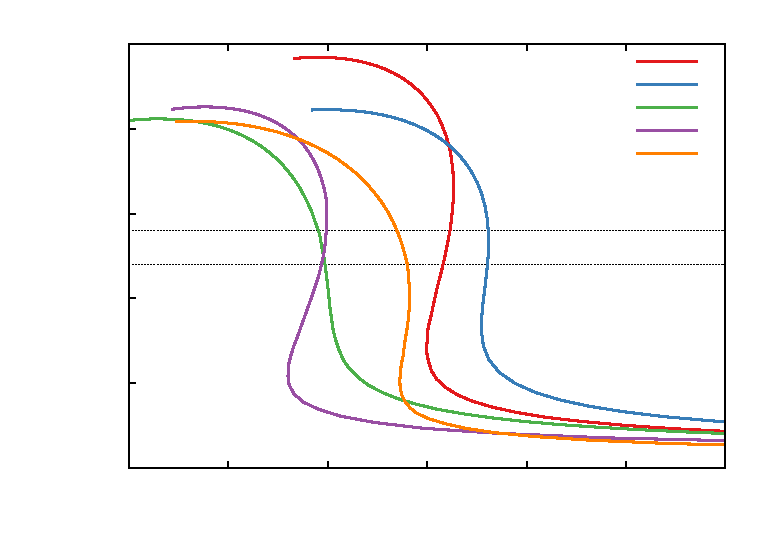
\includegraphics{images/tov-mass-vs-radius}}%
    \gplfronttext
  \end{picture}%
\endgroup

	\caption[Neutron star mass vs. areal radius]{
		ADM neutron star mass vs. areal radius for nuclear equations of state sliced at $T=0.1{\rm MeV}$ in $\beta$-equilibrium.  Intersections of dotted lines and colored curves represent ADM the neutron star masses chosen for this survey: $M_{\rm NS} = (1.2, 1.4) M_{\odot}$.  
	}
	\label{fig:MvsR}
\end{figure}

From the $M-R$ curves in Figure \ref{fig:MvsR} alone, there are a bounty of astrophysics questions we can ask.  
By adopting these finite-temperature, composition-dependent equation of state models for our neutron stars, what observable characterisitics are observed during inspiral and merger?  
How much does the creation of r-process elements in the dynamical outflows vary?  
Does the generated gravitational waveform vary aside from its dependence on the compactness parameter?  
Are the predictions of the fitting formulae~\cite{foucart2012black,pannarale2014black,kawaguchi2016models} of the resulting remnant and ejecta masses correct, even though they were formed with barotropic equations of state?

\begin{figure}
	\centering
	% GNUPLOT: LaTeX picture with Postscript
\begingroup
\newcommand{\ft}[0]{\footnotesize}
  \makeatletter
  \providecommand\color[2][]{%
    \GenericError{(gnuplot) \space\space\space\@spaces}{%
      Package color not loaded in conjunction with
      terminal option `colourtext'%
    }{See the gnuplot documentation for explanation.%
    }{Either use 'blacktext' in gnuplot or load the package
      color.sty in LaTeX.}%
    \renewcommand\color[2][]{}%
  }%
  \providecommand\includegraphics[2][]{%
    \GenericError{(gnuplot) \space\space\space\@spaces}{%
      Package graphicx or graphics not loaded%
    }{See the gnuplot documentation for explanation.%
    }{The gnuplot epslatex terminal needs graphicx.sty or graphics.sty.}%
    \renewcommand\includegraphics[2][]{}%
  }%
  \providecommand\rotatebox[2]{#2}%
  \@ifundefined{ifGPcolor}{%
    \newif\ifGPcolor
    \GPcolortrue
  }{}%
  \@ifundefined{ifGPblacktext}{%
    \newif\ifGPblacktext
    \GPblacktexttrue
  }{}%
  % define a \g@addto@macro without @ in the name:
  \let\gplgaddtomacro\g@addto@macro
  % define empty templates for all commands taking text:
  \gdef\gplbacktext{}%
  \gdef\gplfronttext{}%
  \makeatother
  \ifGPblacktext
    % no textcolor at all
    \def\colorrgb#1{}%
    \def\colorgray#1{}%
  \else
    % gray or color?
    \ifGPcolor
      \def\colorrgb#1{\color[rgb]{#1}}%
      \def\colorgray#1{\color[gray]{#1}}%
      \expandafter\def\csname LTw\endcsname{\color{white}}%
      \expandafter\def\csname LTb\endcsname{\color{black}}%
      \expandafter\def\csname LTa\endcsname{\color{black}}%
      \expandafter\def\csname LT0\endcsname{\color[rgb]{1,0,0}}%
      \expandafter\def\csname LT1\endcsname{\color[rgb]{0,1,0}}%
      \expandafter\def\csname LT2\endcsname{\color[rgb]{0,0,1}}%
      \expandafter\def\csname LT3\endcsname{\color[rgb]{1,0,1}}%
      \expandafter\def\csname LT4\endcsname{\color[rgb]{0,1,1}}%
      \expandafter\def\csname LT5\endcsname{\color[rgb]{1,1,0}}%
      \expandafter\def\csname LT6\endcsname{\color[rgb]{0,0,0}}%
      \expandafter\def\csname LT7\endcsname{\color[rgb]{1,0.3,0}}%
      \expandafter\def\csname LT8\endcsname{\color[rgb]{0.5,0.5,0.5}}%
    \else
      % gray
      \def\colorrgb#1{\color{black}}%
      \def\colorgray#1{\color[gray]{#1}}%
      \expandafter\def\csname LTw\endcsname{\color{white}}%
      \expandafter\def\csname LTb\endcsname{\color{black}}%
      \expandafter\def\csname LTa\endcsname{\color{black}}%
      \expandafter\def\csname LT0\endcsname{\color{black}}%
      \expandafter\def\csname LT1\endcsname{\color{black}}%
      \expandafter\def\csname LT2\endcsname{\color{black}}%
      \expandafter\def\csname LT3\endcsname{\color{black}}%
      \expandafter\def\csname LT4\endcsname{\color{black}}%
      \expandafter\def\csname LT5\endcsname{\color{black}}%
      \expandafter\def\csname LT6\endcsname{\color{black}}%
      \expandafter\def\csname LT7\endcsname{\color{black}}%
      \expandafter\def\csname LT8\endcsname{\color{black}}%
    \fi
  \fi
  \setlength{\unitlength}{0.0500bp}%
  \begin{picture}(7200.00,5040.00)%
    \gplgaddtomacro\gplbacktext{%
      \csname LTb\endcsname%
      \put(1210,820){\makebox(0,0)[r]{\strut{} 1e+27}}%
      \put(1210,1272){\makebox(0,0)[r]{\strut{} 1e+28}}%
      \put(1210,1724){\makebox(0,0)[r]{\strut{} 1e+29}}%
      \put(1210,2177){\makebox(0,0)[r]{\strut{} 1e+30}}%
      \put(1210,2629){\makebox(0,0)[r]{\strut{} 1e+31}}%
      \put(1210,3081){\makebox(0,0)[r]{\strut{} 1e+32}}%
      \put(1210,3534){\makebox(0,0)[r]{\strut{} 1e+33}}%
      \put(1210,3986){\makebox(0,0)[r]{\strut{} 1e+34}}%
      \put(1210,4438){\makebox(0,0)[r]{\strut{} 1e+35}}%
      \put(1571,484){\makebox(0,0){\strut{} 1e+11}}%
      \put(2663,484){\makebox(0,0){\strut{} 1e+12}}%
      \put(3755,484){\makebox(0,0){\strut{} 1e+13}}%
      \put(4847,484){\makebox(0,0){\strut{} 1e+14}}%
      \put(5939,484){\makebox(0,0){\strut{} 1e+15}}%
      \put(176,2739){\rotatebox{-270}{\makebox(0,0){\strut{}Pressure (barye)}}}%
      \put(4072,154){\makebox(0,0){\strut{}Density (g/cm$^3$)}}%
    }%
    \gplgaddtomacro\gplfronttext{%
      \csname LTb\endcsname%
      \put(2329,4602){\makebox(0,0)[l]{\strut{}Hempel DD2}}%
      \csname LTb\endcsname%
      \put(2329,4382){\makebox(0,0)[l]{\strut{}G. Shen FSU 2.1}}%
      \csname LTb\endcsname%
      \put(2329,4162){\makebox(0,0)[l]{\strut{}SFHo}}%
      \csname LTb\endcsname%
      \put(2329,3942){\makebox(0,0)[l]{\strut{}SFHx}}%
      \csname LTb\endcsname%
      \put(2329,3722){\makebox(0,0)[l]{\strut{}LS220}}%
    }%
    \gplbacktext
    \put(0,0){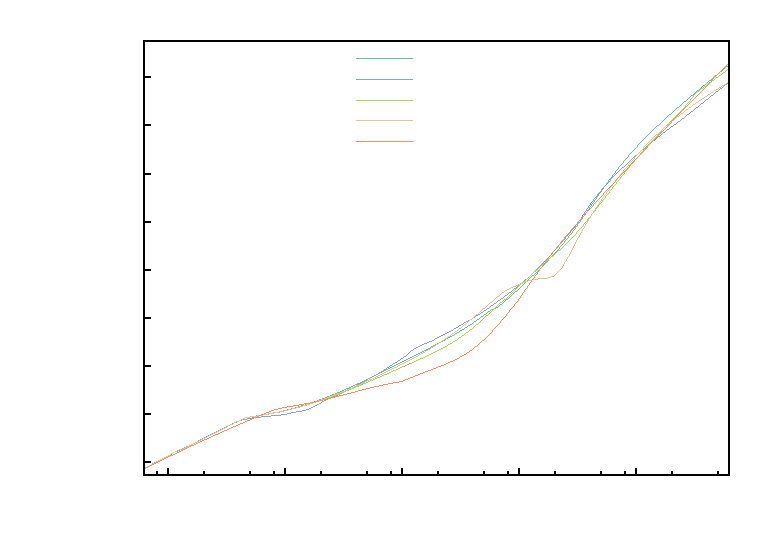
\includegraphics{images/pressure-vs-density}}%
    \gplfronttext
  \end{picture}%
\endgroup

	\caption[Pressure vs. density for a cold, beta-equilibrium slice]{
		Pressure vs. density for finite-temperature, nuclear equations of state used in this study. The initial fluid is chosen to be cold and in $\beta$-equilibrium: $T=0.1 {\rm MeV}$ and $Y_e = Y_e (n_b)$, respectively.  Vertical dotted line represents the fiducial density.
	}
	\label{fig:PvsRho}
\end{figure}

In Figure \ref{fig:PvsRho}, it can be seen that the relationship between pressure and density at low densities is similar to a $\Gamma \approx 2$ polytrope in the ``cold'' regime of the table.  
Qualitatively, the pressure support at lower densities can be stronger for one equation of state, but softer at higher densities compared to another.  
Indeed, it was noted in~\cite{steiner2013core} that the concept of describing an equation of state as stiff or soft can be somewhat misleading.  
That is, the effective adiabatic index $\tilde{\Gamma}$ of Equation \ref{e:adiabat} for the poofier FSU2.1 model is smaller (larger) in the lower (higher) density regions compared to the more compact SFHo in the ``cold'' phase.

%\begin{figure}
%	\centering
%	% GNUPLOT: LaTeX picture with Postscript
\begingroup
  \makeatletter
  \providecommand\color[2][]{%
    \GenericError{(gnuplot) \space\space\space\@spaces}{%
      Package color not loaded in conjunction with
      terminal option `colourtext'%
    }{See the gnuplot documentation for explanation.%
    }{Either use 'blacktext' in gnuplot or load the package
      color.sty in LaTeX.}%
    \renewcommand\color[2][]{}%
  }%
  \providecommand\includegraphics[2][]{%
    \GenericError{(gnuplot) \space\space\space\@spaces}{%
      Package graphicx or graphics not loaded%
    }{See the gnuplot documentation for explanation.%
    }{The gnuplot epslatex terminal needs graphicx.sty or graphics.sty.}%
    \renewcommand\includegraphics[2][]{}%
  }%
  \providecommand\rotatebox[2]{#2}%
  \@ifundefined{ifGPcolor}{%
    \newif\ifGPcolor
    \GPcolortrue
  }{}%
  \@ifundefined{ifGPblacktext}{%
    \newif\ifGPblacktext
    \GPblacktexttrue
  }{}%
  % define a \g@addto@macro without @ in the name:
  \let\gplgaddtomacro\g@addto@macro
  % define empty templates for all commands taking text:
  \gdef\gplbacktext{}%
  \gdef\gplfronttext{}%
  \makeatother
  \ifGPblacktext
    % no textcolor at all
    \def\colorrgb#1{}%
    \def\colorgray#1{}%
  \else
    % gray or color?
    \ifGPcolor
      \def\colorrgb#1{\color[rgb]{#1}}%
      \def\colorgray#1{\color[gray]{#1}}%
      \expandafter\def\csname LTw\endcsname{\color{white}}%
      \expandafter\def\csname LTb\endcsname{\color{black}}%
      \expandafter\def\csname LTa\endcsname{\color{black}}%
      \expandafter\def\csname LT0\endcsname{\color[rgb]{1,0,0}}%
      \expandafter\def\csname LT1\endcsname{\color[rgb]{0,1,0}}%
      \expandafter\def\csname LT2\endcsname{\color[rgb]{0,0,1}}%
      \expandafter\def\csname LT3\endcsname{\color[rgb]{1,0,1}}%
      \expandafter\def\csname LT4\endcsname{\color[rgb]{0,1,1}}%
      \expandafter\def\csname LT5\endcsname{\color[rgb]{1,1,0}}%
      \expandafter\def\csname LT6\endcsname{\color[rgb]{0,0,0}}%
      \expandafter\def\csname LT7\endcsname{\color[rgb]{1,0.3,0}}%
      \expandafter\def\csname LT8\endcsname{\color[rgb]{0.5,0.5,0.5}}%
    \else
      % gray
      \def\colorrgb#1{\color{black}}%
      \def\colorgray#1{\color[gray]{#1}}%
      \expandafter\def\csname LTw\endcsname{\color{white}}%
      \expandafter\def\csname LTb\endcsname{\color{black}}%
      \expandafter\def\csname LTa\endcsname{\color{black}}%
      \expandafter\def\csname LT0\endcsname{\color{black}}%
      \expandafter\def\csname LT1\endcsname{\color{black}}%
      \expandafter\def\csname LT2\endcsname{\color{black}}%
      \expandafter\def\csname LT3\endcsname{\color{black}}%
      \expandafter\def\csname LT4\endcsname{\color{black}}%
      \expandafter\def\csname LT5\endcsname{\color{black}}%
      \expandafter\def\csname LT6\endcsname{\color{black}}%
      \expandafter\def\csname LT7\endcsname{\color{black}}%
      \expandafter\def\csname LT8\endcsname{\color{black}}%
    \fi
  \fi
  \setlength{\unitlength}{0.0500bp}%
  \begin{picture}(7200.00,5040.00)%
    \gplgaddtomacro\gplbacktext{%
      \csname LTb\endcsname%
      \put(946,704){\makebox(0,0)[r]{\strut{} 0}}%
      \put(946,1111){\makebox(0,0)[r]{\strut{} 0.1}}%
      \put(946,1518){\makebox(0,0)[r]{\strut{} 0.2}}%
      \put(946,1925){\makebox(0,0)[r]{\strut{} 0.3}}%
      \put(946,2332){\makebox(0,0)[r]{\strut{} 0.4}}%
      \put(946,2739){\makebox(0,0)[r]{\strut{} 0.5}}%
      \put(946,3147){\makebox(0,0)[r]{\strut{} 0.6}}%
      \put(946,3554){\makebox(0,0)[r]{\strut{} 0.7}}%
      \put(946,3961){\makebox(0,0)[r]{\strut{} 0.8}}%
      \put(946,4368){\makebox(0,0)[r]{\strut{} 0.9}}%
      \put(946,4775){\makebox(0,0)[r]{\strut{} 1}}%
      \put(1318,484){\makebox(0,0){\strut{} 1e+11}}%
      \put(2463,484){\makebox(0,0){\strut{} 1e+12}}%
      \put(3608,484){\makebox(0,0){\strut{} 1e+13}}%
      \put(4753,484){\makebox(0,0){\strut{} 1e+14}}%
      \put(5898,484){\makebox(0,0){\strut{} 1e+15}}%
      \put(176,2739){\rotatebox{-270}{\makebox(0,0){\strut{}$[P(T) - P(0)]/P(T)$}}}%
      \put(3940,154){\makebox(0,0){\strut{}Density (g/cm$^3$)}}%
    }%
    \gplgaddtomacro\gplfronttext{%
      \csname LTb\endcsname%
      \put(2065,1757){\makebox(0,0)[l]{\strut{}Hempel DD2}}%
      \csname LTb\endcsname%
      \put(2065,1537){\makebox(0,0)[l]{\strut{}G. Shen FSU 2.1}}%
      \csname LTb\endcsname%
      \put(2065,1317){\makebox(0,0)[l]{\strut{}SFHo}}%
      \csname LTb\endcsname%
      \put(2065,1097){\makebox(0,0)[l]{\strut{}SFHx}}%
      \csname LTb\endcsname%
      \put(2065,877){\makebox(0,0)[l]{\strut{}LS220}}%
    }%
    \gplbacktext
    \put(0,0){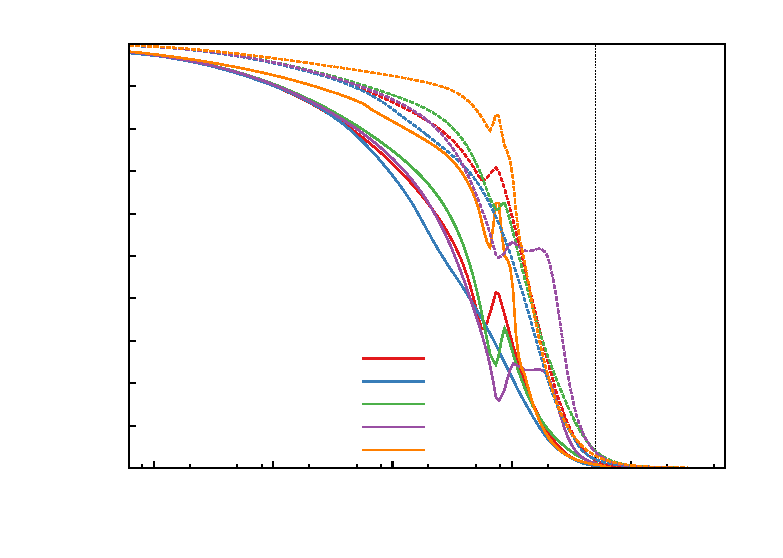
\includegraphics{images/delta-pressure-vs-density}}%
    \gplfronttext
  \end{picture}%
\endgroup

%	\caption[Difference in pressure vs. density for constant $Y_e$, varying temperature]{
%		Normalized pressure difference at $Y_e = 0.05$ between $T = (0,5) {\rm MeV}$ (solid) and $T = (0,10) {\rm MeV}$ (dashed), both normalized by the zero-temperature pressure. Vertical dotted line represents the fiducial density.
%	}
%	\label{fig:dPvsRho}
%\end{figure}


%\begin{figure}
%	\centering
%	% GNUPLOT: LaTeX picture with Postscript
\begingroup
\newcommand{\ft}[0]{\footnotesize}
  \makeatletter
  \providecommand\color[2][]{%
    \GenericError{(gnuplot) \space\space\space\@spaces}{%
      Package color not loaded in conjunction with
      terminal option `colourtext'%
    }{See the gnuplot documentation for explanation.%
    }{Either use 'blacktext' in gnuplot or load the package
      color.sty in LaTeX.}%
    \renewcommand\color[2][]{}%
  }%
  \providecommand\includegraphics[2][]{%
    \GenericError{(gnuplot) \space\space\space\@spaces}{%
      Package graphicx or graphics not loaded%
    }{See the gnuplot documentation for explanation.%
    }{The gnuplot epslatex terminal needs graphicx.sty or graphics.sty.}%
    \renewcommand\includegraphics[2][]{}%
  }%
  \providecommand\rotatebox[2]{#2}%
  \@ifundefined{ifGPcolor}{%
    \newif\ifGPcolor
    \GPcolortrue
  }{}%
  \@ifundefined{ifGPblacktext}{%
    \newif\ifGPblacktext
    \GPblacktexttrue
  }{}%
  % define a \g@addto@macro without @ in the name:
  \let\gplgaddtomacro\g@addto@macro
  % define empty templates for all commands taking text:
  \gdef\gplbacktext{}%
  \gdef\gplfronttext{}%
  \makeatother
  \ifGPblacktext
    % no textcolor at all
    \def\colorrgb#1{}%
    \def\colorgray#1{}%
  \else
    % gray or color?
    \ifGPcolor
      \def\colorrgb#1{\color[rgb]{#1}}%
      \def\colorgray#1{\color[gray]{#1}}%
      \expandafter\def\csname LTw\endcsname{\color{white}}%
      \expandafter\def\csname LTb\endcsname{\color{black}}%
      \expandafter\def\csname LTa\endcsname{\color{black}}%
      \expandafter\def\csname LT0\endcsname{\color[rgb]{1,0,0}}%
      \expandafter\def\csname LT1\endcsname{\color[rgb]{0,1,0}}%
      \expandafter\def\csname LT2\endcsname{\color[rgb]{0,0,1}}%
      \expandafter\def\csname LT3\endcsname{\color[rgb]{1,0,1}}%
      \expandafter\def\csname LT4\endcsname{\color[rgb]{0,1,1}}%
      \expandafter\def\csname LT5\endcsname{\color[rgb]{1,1,0}}%
      \expandafter\def\csname LT6\endcsname{\color[rgb]{0,0,0}}%
      \expandafter\def\csname LT7\endcsname{\color[rgb]{1,0.3,0}}%
      \expandafter\def\csname LT8\endcsname{\color[rgb]{0.5,0.5,0.5}}%
    \else
      % gray
      \def\colorrgb#1{\color{black}}%
      \def\colorgray#1{\color[gray]{#1}}%
      \expandafter\def\csname LTw\endcsname{\color{white}}%
      \expandafter\def\csname LTb\endcsname{\color{black}}%
      \expandafter\def\csname LTa\endcsname{\color{black}}%
      \expandafter\def\csname LT0\endcsname{\color{black}}%
      \expandafter\def\csname LT1\endcsname{\color{black}}%
      \expandafter\def\csname LT2\endcsname{\color{black}}%
      \expandafter\def\csname LT3\endcsname{\color{black}}%
      \expandafter\def\csname LT4\endcsname{\color{black}}%
      \expandafter\def\csname LT5\endcsname{\color{black}}%
      \expandafter\def\csname LT6\endcsname{\color{black}}%
      \expandafter\def\csname LT7\endcsname{\color{black}}%
      \expandafter\def\csname LT8\endcsname{\color{black}}%
    \fi
  \fi
  \setlength{\unitlength}{0.0500bp}%
  \begin{picture}(7200.00,5040.00)%
    \gplgaddtomacro\gplbacktext{%
      \csname LTb\endcsname%
      \put(682,704){\makebox(0,0)[r]{\strut{} 0}}%
      \put(682,1518){\makebox(0,0)[r]{\strut{} 1}}%
      \put(682,2332){\makebox(0,0)[r]{\strut{} 2}}%
      \put(682,3147){\makebox(0,0)[r]{\strut{} 3}}%
      \put(682,3961){\makebox(0,0)[r]{\strut{} 4}}%
      \put(682,4775){\makebox(0,0)[r]{\strut{} 5}}%
      \put(1065,484){\makebox(0,0){\strut{} 1e+11}}%
      \put(2263,484){\makebox(0,0){\strut{} 1e+12}}%
      \put(3460,484){\makebox(0,0){\strut{} 1e+13}}%
      \put(4658,484){\makebox(0,0){\strut{} 1e+14}}%
      \put(5856,484){\makebox(0,0){\strut{} 1e+15}}%
      \put(176,2739){\rotatebox{-270}{\makebox(0,0){\strut{}$\tilde{\Gamma}$}}}%
      \put(3808,154){\makebox(0,0){\strut{}Density (g/cm$^3$)}}%
    }%
    \gplgaddtomacro\gplfronttext{%
      \csname LTb\endcsname%
      \put(1801,4602){\makebox(0,0)[l]{\strut{}Hempel DD2}}%
      \csname LTb\endcsname%
      \put(1801,4382){\makebox(0,0)[l]{\strut{}G. Shen FSU 2.1}}%
      \csname LTb\endcsname%
      \put(1801,4162){\makebox(0,0)[l]{\strut{}SFHo}}%
      \csname LTb\endcsname%
      \put(1801,3942){\makebox(0,0)[l]{\strut{}SFHx}}%
      \csname LTb\endcsname%
      \put(1801,3722){\makebox(0,0)[l]{\strut{}LS220}}%
    }%
    \gplbacktext
    \put(0,0){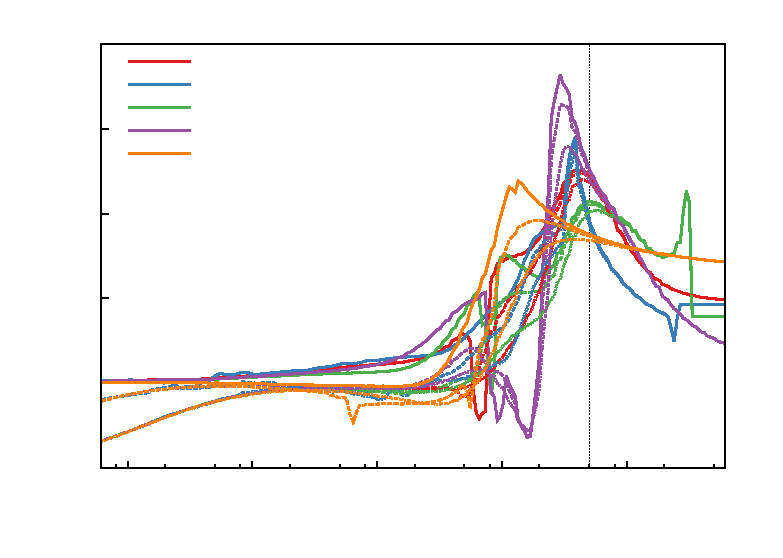
\includegraphics{images/gamma-vs-density}}%
    \gplfronttext
  \end{picture}%
\endgroup

%	\caption[Adiabatic index vs. density for constant $Y_e$, varying temperature]
%	{
%	}
%	\label{fig:GammavsRho}
%\end{figure}


In Figure \ref{fig:MultGammavsRho}, we observe the effect temperature has on the pressure-density relations.  Past the fiducial density $\rho_s = 10^{14.7} {\rm g \, cm^{-3}}$ (with fixed $Y_e = 0.05$), changes in temperature up to $10$MeV do not alter the pressure-density relation by much at all.  As temperature increases in the lower density regime, the structures begin to converge and increase to similar $\tilde{\Gamma}$ between models.  The main differences occur in the intermediate region, where the increasing variance in $\tilde{\Gamma}$ between temperatures becomes clear.

\begin{figure}
	\centering
	% GNUPLOT: LaTeX picture with Postscript
\begingroup
  \makeatletter
  \providecommand\color[2][]{%
    \GenericError{(gnuplot) \space\space\space\@spaces}{%
      Package color not loaded in conjunction with
      terminal option `colourtext'%
    }{See the gnuplot documentation for explanation.%
    }{Either use 'blacktext' in gnuplot or load the package
      color.sty in LaTeX.}%
    \renewcommand\color[2][]{}%
  }%
  \providecommand\includegraphics[2][]{%
    \GenericError{(gnuplot) \space\space\space\@spaces}{%
      Package graphicx or graphics not loaded%
    }{See the gnuplot documentation for explanation.%
    }{The gnuplot epslatex terminal needs graphicx.sty or graphics.sty.}%
    \renewcommand\includegraphics[2][]{}%
  }%
  \providecommand\rotatebox[2]{#2}%
  \@ifundefined{ifGPcolor}{%
    \newif\ifGPcolor
    \GPcolortrue
  }{}%
  \@ifundefined{ifGPblacktext}{%
    \newif\ifGPblacktext
    \GPblacktexttrue
  }{}%
  % define a \g@addto@macro without @ in the name:
  \let\gplgaddtomacro\g@addto@macro
  % define empty templates for all commands taking text:
  \gdef\gplbacktext{}%
  \gdef\gplfronttext{}%
  \makeatother
  \ifGPblacktext
    % no textcolor at all
    \def\colorrgb#1{}%
    \def\colorgray#1{}%
  \else
    % gray or color?
    \ifGPcolor
      \def\colorrgb#1{\color[rgb]{#1}}%
      \def\colorgray#1{\color[gray]{#1}}%
      \expandafter\def\csname LTw\endcsname{\color{white}}%
      \expandafter\def\csname LTb\endcsname{\color{black}}%
      \expandafter\def\csname LTa\endcsname{\color{black}}%
      \expandafter\def\csname LT0\endcsname{\color[rgb]{1,0,0}}%
      \expandafter\def\csname LT1\endcsname{\color[rgb]{0,1,0}}%
      \expandafter\def\csname LT2\endcsname{\color[rgb]{0,0,1}}%
      \expandafter\def\csname LT3\endcsname{\color[rgb]{1,0,1}}%
      \expandafter\def\csname LT4\endcsname{\color[rgb]{0,1,1}}%
      \expandafter\def\csname LT5\endcsname{\color[rgb]{1,1,0}}%
      \expandafter\def\csname LT6\endcsname{\color[rgb]{0,0,0}}%
      \expandafter\def\csname LT7\endcsname{\color[rgb]{1,0.3,0}}%
      \expandafter\def\csname LT8\endcsname{\color[rgb]{0.5,0.5,0.5}}%
    \else
      % gray
      \def\colorrgb#1{\color{black}}%
      \def\colorgray#1{\color[gray]{#1}}%
      \expandafter\def\csname LTw\endcsname{\color{white}}%
      \expandafter\def\csname LTb\endcsname{\color{black}}%
      \expandafter\def\csname LTa\endcsname{\color{black}}%
      \expandafter\def\csname LT0\endcsname{\color{black}}%
      \expandafter\def\csname LT1\endcsname{\color{black}}%
      \expandafter\def\csname LT2\endcsname{\color{black}}%
      \expandafter\def\csname LT3\endcsname{\color{black}}%
      \expandafter\def\csname LT4\endcsname{\color{black}}%
      \expandafter\def\csname LT5\endcsname{\color{black}}%
      \expandafter\def\csname LT6\endcsname{\color{black}}%
      \expandafter\def\csname LT7\endcsname{\color{black}}%
      \expandafter\def\csname LT8\endcsname{\color{black}}%
    \fi
  \fi
  \setlength{\unitlength}{0.0500bp}%
  \begin{picture}(7200.00,5040.00)%
    \gplgaddtomacro\gplbacktext{%
      \csname LTb\endcsname%
      \put(682,704){\makebox(0,0)[r]{\strut{} 0}}%
      \put(682,1518){\makebox(0,0)[r]{\strut{} 1}}%
      \put(682,2332){\makebox(0,0)[r]{\strut{} 2}}%
      \put(682,3147){\makebox(0,0)[r]{\strut{} 3}}%
      \put(682,3961){\makebox(0,0)[r]{\strut{} 4}}%
      \put(682,4775){\makebox(0,0)[r]{\strut{} 5}}%
      \put(1065,484){\makebox(0,0){\strut{} 1e+11}}%
      \put(2263,484){\makebox(0,0){\strut{} 1e+12}}%
      \put(3460,484){\makebox(0,0){\strut{} 1e+13}}%
      \put(4658,484){\makebox(0,0){\strut{} 1e+14}}%
      \put(5856,484){\makebox(0,0){\strut{} 1e+15}}%
      \put(176,2739){\rotatebox{-270}{\makebox(0,0){\strut{}$\tilde{\Gamma}$}}}%
      \put(3808,154){\makebox(0,0){\strut{}Density (g/cm$^3$)}}%
      \put(5613,3961){\rotatebox{90}{\makebox(0,0)[l]{\strut{}\small $\rho_{\rm fid}$}}}%
    }%
    \gplgaddtomacro\gplfronttext{%
      \csname LTb\endcsname%
      \put(1801,4602){\makebox(0,0)[l]{\strut{}Hempel DD2}}%
      \csname LTb\endcsname%
      \put(1801,4382){\makebox(0,0)[l]{\strut{}G. Shen FSU 2.1}}%
      \csname LTb\endcsname%
      \put(1801,4162){\makebox(0,0)[l]{\strut{}SFHo}}%
      \csname LTb\endcsname%
      \put(1801,3942){\makebox(0,0)[l]{\strut{}SFHx}}%
      \csname LTb\endcsname%
      \put(1801,3722){\makebox(0,0)[l]{\strut{}LS220}}%
      \csname LTb\endcsname%
      \put(5025,3961){\rotatebox{90}{\makebox(0,0)[l]{\strut{}\small $\rho_{\rm sat}$}}}%
      \put(5857,1635){\makebox(0,0)[l]{\strut{}\small $\tilde{\Gamma} = 4/3$}}%
    }%
    \gplbacktext
    \put(0,0){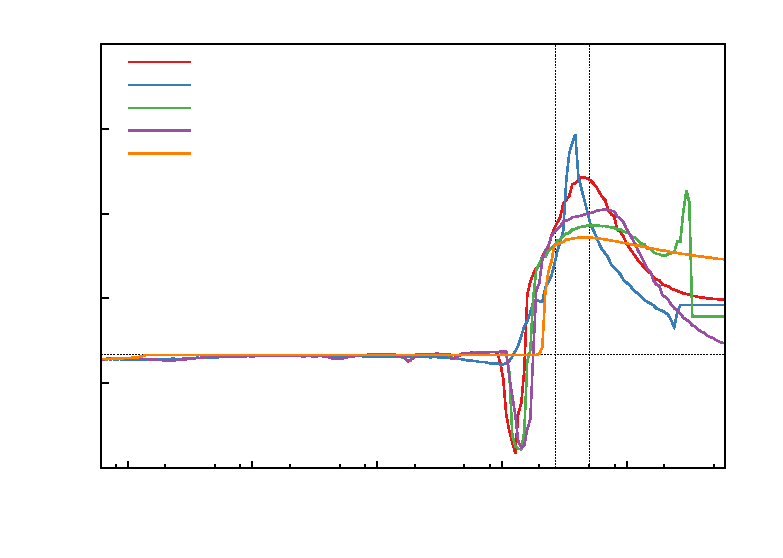
\includegraphics{images/one-gamma-vs-density}}%
    \gplfronttext
  \end{picture}%
\endgroup

	\caption[Adiabatic index vs. density for constant composition and temperature]
	{
		Effective adiabatic index as a function of baryon density for constant $Y_e = 0.3$ and temperature $T = 0.7 {\rm MeV}$, for comparison to the literature~\cite{Fischer2014}.  Displayed are vertical lines for the critical density $\rho_c$ and fiducial density $\rho_{\rm fid}$, while the third vertical line to the right is the nuclear saturation density.  The horizontal line corresponds to a $\Gamma = 4/3$ polytrope law.
	}
	\label{fig:OneGammavsRho}
\end{figure}


\begin{figure}[]
	\centering
	\footnotesize{	
		% GNUPLOT: LaTeX picture with Postscript
\begingroup
\newcommand{\ft}[0]{\footnotesize}
  \makeatletter
  \providecommand\color[2][]{%
    \GenericError{(gnuplot) \space\space\space\@spaces}{%
      Package color not loaded in conjunction with
      terminal option `colourtext'%
    }{See the gnuplot documentation for explanation.%
    }{Either use 'blacktext' in gnuplot or load the package
      color.sty in LaTeX.}%
    \renewcommand\color[2][]{}%
  }%
  \providecommand\includegraphics[2][]{%
    \GenericError{(gnuplot) \space\space\space\@spaces}{%
      Package graphicx or graphics not loaded%
    }{See the gnuplot documentation for explanation.%
    }{The gnuplot epslatex terminal needs graphicx.sty or graphics.sty.}%
    \renewcommand\includegraphics[2][]{}%
  }%
  \providecommand\rotatebox[2]{#2}%
  \@ifundefined{ifGPcolor}{%
    \newif\ifGPcolor
    \GPcolortrue
  }{}%
  \@ifundefined{ifGPblacktext}{%
    \newif\ifGPblacktext
    \GPblacktexttrue
  }{}%
  % define a \g@addto@macro without @ in the name:
  \let\gplgaddtomacro\g@addto@macro
  % define empty templates for all commands taking text:
  \gdef\gplbacktext{}%
  \gdef\gplfronttext{}%
  \makeatother
  \ifGPblacktext
    % no textcolor at all
    \def\colorrgb#1{}%
    \def\colorgray#1{}%
  \else
    % gray or color?
    \ifGPcolor
      \def\colorrgb#1{\color[rgb]{#1}}%
      \def\colorgray#1{\color[gray]{#1}}%
      \expandafter\def\csname LTw\endcsname{\color{white}}%
      \expandafter\def\csname LTb\endcsname{\color{black}}%
      \expandafter\def\csname LTa\endcsname{\color{black}}%
      \expandafter\def\csname LT0\endcsname{\color[rgb]{1,0,0}}%
      \expandafter\def\csname LT1\endcsname{\color[rgb]{0,1,0}}%
      \expandafter\def\csname LT2\endcsname{\color[rgb]{0,0,1}}%
      \expandafter\def\csname LT3\endcsname{\color[rgb]{1,0,1}}%
      \expandafter\def\csname LT4\endcsname{\color[rgb]{0,1,1}}%
      \expandafter\def\csname LT5\endcsname{\color[rgb]{1,1,0}}%
      \expandafter\def\csname LT6\endcsname{\color[rgb]{0,0,0}}%
      \expandafter\def\csname LT7\endcsname{\color[rgb]{1,0.3,0}}%
      \expandafter\def\csname LT8\endcsname{\color[rgb]{0.5,0.5,0.5}}%
    \else
      % gray
      \def\colorrgb#1{\color{black}}%
      \def\colorgray#1{\color[gray]{#1}}%
      \expandafter\def\csname LTw\endcsname{\color{white}}%
      \expandafter\def\csname LTb\endcsname{\color{black}}%
      \expandafter\def\csname LTa\endcsname{\color{black}}%
      \expandafter\def\csname LT0\endcsname{\color{black}}%
      \expandafter\def\csname LT1\endcsname{\color{black}}%
      \expandafter\def\csname LT2\endcsname{\color{black}}%
      \expandafter\def\csname LT3\endcsname{\color{black}}%
      \expandafter\def\csname LT4\endcsname{\color{black}}%
      \expandafter\def\csname LT5\endcsname{\color{black}}%
      \expandafter\def\csname LT6\endcsname{\color{black}}%
      \expandafter\def\csname LT7\endcsname{\color{black}}%
      \expandafter\def\csname LT8\endcsname{\color{black}}%
    \fi
  \fi
  \setlength{\unitlength}{0.0500bp}%
  \begin{picture}(8640.00,6552.00)%
    \gplgaddtomacro\gplbacktext{%
      \csname LTb\endcsname%
      \put(732,3276){\makebox(0,0)[r]{\strut{}0}}%
      \put(732,3822){\makebox(0,0)[r]{\strut{}1}}%
      \put(732,4367){\makebox(0,0)[r]{\strut{}2}}%
      \put(732,4913){\makebox(0,0)[r]{\strut{}3}}%
      \put(732,5459){\makebox(0,0)[r]{\strut{}4}}%
      \put(1009,3056){\makebox(0,0){\strut{}}}%
      \put(1700,3056){\makebox(0,0){\strut{}}}%
      \put(2391,3056){\makebox(0,0){\strut{}}}%
      \put(3082,3056){\makebox(0,0){\strut{}}}%
      \put(3773,3056){\makebox(0,0){\strut{}}}%
      \put(4043,5633){\makebox(0,0)[l]{\strut{}a}}%
    }%
    \gplgaddtomacro\gplfronttext{%
      \csname LTb\endcsname%
      \put(1851,5722){\makebox(0,0)[l]{\strut{}Hempel DD2}}%
      \csname LTb\endcsname%
      \put(1851,5502){\makebox(0,0)[l]{\strut{}G. Shen FSU 2.1}}%
      \csname LTb\endcsname%
      \put(1851,5282){\makebox(0,0)[l]{\strut{}SFHo}}%
      \csname LTb\endcsname%
      \put(1851,5062){\makebox(0,0)[l]{\strut{}SFHx}}%
      \csname LTb\endcsname%
      \put(1851,4842){\makebox(0,0)[l]{\strut{}LS220}}%
    }%
    \gplgaddtomacro\gplbacktext{%
      \csname LTb\endcsname%
      \put(4188,3276){\makebox(0,0)[r]{\strut{}}}%
      \put(4188,3822){\makebox(0,0)[r]{\strut{}}}%
      \put(4188,4367){\makebox(0,0)[r]{\strut{}}}%
      \put(4188,4913){\makebox(0,0)[r]{\strut{}}}%
      \put(4188,5459){\makebox(0,0)[r]{\strut{}}}%
      \put(4465,3056){\makebox(0,0){\strut{}}}%
      \put(5156,3056){\makebox(0,0){\strut{}}}%
      \put(5847,3056){\makebox(0,0){\strut{}}}%
      \put(6538,3056){\makebox(0,0){\strut{}}}%
      \put(7229,3056){\makebox(0,0){\strut{}}}%
      \put(7499,5633){\makebox(0,0)[l]{\strut{}b}}%
    }%
    \gplgaddtomacro\gplfronttext{%
    }%
    \gplgaddtomacro\gplbacktext{%
      \csname LTb\endcsname%
      \put(732,655){\makebox(0,0)[r]{\strut{}0}}%
      \put(732,1201){\makebox(0,0)[r]{\strut{}1}}%
      \put(732,1747){\makebox(0,0)[r]{\strut{}2}}%
      \put(732,2293){\makebox(0,0)[r]{\strut{}3}}%
      \put(732,2838){\makebox(0,0)[r]{\strut{}4}}%
      \put(1009,435){\makebox(0,0){\strut{} 1e+11}}%
      \put(1700,435){\makebox(0,0){\strut{} 1e+12}}%
      \put(2391,435){\makebox(0,0){\strut{} 1e+13}}%
      \put(3082,435){\makebox(0,0){\strut{} 1e+14}}%
      \put(3773,435){\makebox(0,0){\strut{} 1e+15}}%
      \put(4043,3013){\makebox(0,0)[l]{\strut{}c}}%
    }%
    \gplgaddtomacro\gplfronttext{%
    }%
    \gplgaddtomacro\gplbacktext{%
      \csname LTb\endcsname%
      \put(4188,655){\makebox(0,0)[r]{\strut{}}}%
      \put(4188,1201){\makebox(0,0)[r]{\strut{}}}%
      \put(4188,1747){\makebox(0,0)[r]{\strut{}}}%
      \put(4188,2293){\makebox(0,0)[r]{\strut{}}}%
      \put(4188,2838){\makebox(0,0)[r]{\strut{}}}%
      \put(4465,435){\makebox(0,0){\strut{} 1e+11}}%
      \put(5156,435){\makebox(0,0){\strut{} 1e+12}}%
      \put(5847,435){\makebox(0,0){\strut{} 1e+13}}%
      \put(6538,435){\makebox(0,0){\strut{} 1e+14}}%
      \put(7229,435){\makebox(0,0){\strut{} 1e+15}}%
      \put(491,3275){\rotatebox{-270}{\makebox(0,0){\strut{}$\tilde{\Gamma}$}}}%
      \put(4319,105){\makebox(0,0){\strut{}$\rho_0$ (g/cm$^3$)}}%
      \put(7499,3013){\makebox(0,0)[l]{\strut{}d}}%
    }%
    \gplgaddtomacro\gplfronttext{%
    }%
    \gplbacktext
    \put(0,0){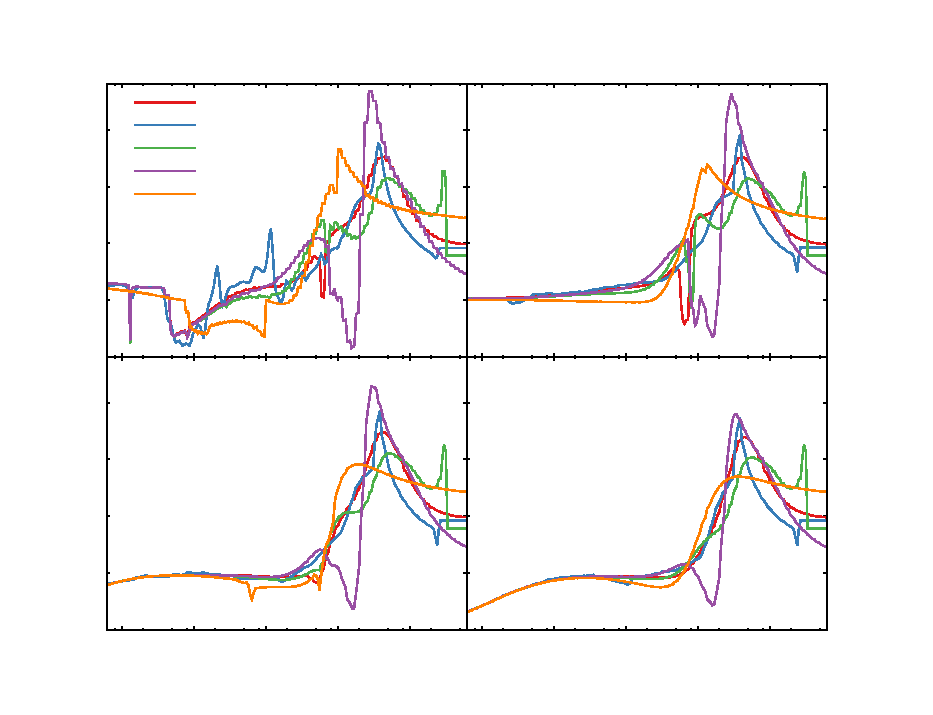
\includegraphics{images/mp-gamma-vs-density}}%
    \gplfronttext
  \end{picture}%
\endgroup

	}
	\caption[Adiabatic index vs. density for constant $Y_e = 0.3$, varying temperature]
	{
		Effective adiabatic index as a function of density for the equaions of state considered, sliced along 
		(a) cold $T=0.1 {\rm MeV}$, $\beta$-equilibrium,
		(b) temperature $T=0 {\rm MeV}$,
		(c) $T=5{\rm MeV}$,
		(d) $T=10{\rm MeV}$,
		where cases (b)-(d) also assume very neutron rich composition $Y_e = 0.05$.  In all models, as atmosphere temperature increases the equations of state all begin to soften and become less distinguishable.  
		The step-effect in (a) is likely the result of a low resolution used in the $\beta$-equilibrium slice. 
	}
	\label{fig:MultGammavsRho}
\end{figure}


% Numerical Methods
\chapter{Numerical Methods}
\label{chap:chapter-3}
	
Simulating compact binary coalescence requires Einstein's full theory of general relativity.
We approach the problem of evolving black hole-neutron star inspirals and mergers with the Spectral Einstein Code (\SpEC).  
\SpEC, as in other codes [cite], uses a two-grid method to simultaneously evolve Einstein's equations and the fluid equations.
We evolve Einstein's equations using multi-domain pseudospectral methods on what we'll refer to as the GR grid.
For the fluid matter, we evolve the fluid equations on a multi-domain finite volume grid, occasionally referred to in this work as the fluid grid.

In Section \ref{sec:gr-grid}, we discuss the design implementation we use to evolve Einstein's equations with pseudospectral methods in \SpEC.  The finite difference scheme used to evolve the fluid equations is discussed in Section \ref{sec:fd-grid}.  The grid-to-grid communication and time stepping procedure is discussed in Section \ref{sec:communication}.  The implementation of our new mesh refinement algorithm for evolving the FD grid will be discussed in Section \ref{sec:hydro-amr}.  We discuss the necessary refinements to the grids in Section \ref{sec:epochs}.

\section{GR Grid}
\label{sec:gr-grid}

In \SpEC, we use the generalized harmonic formulation of Einstein's field equations.  By harmonic, we assume the coordinates $x^\alpha$ obey the inhomogeneous  wave equation
\begin{equation}
g_{ab} \nabla^c \nabla_c x^b = H_a (x, g_{ab})
\end{equation}
for some generic, harmonic gauge function $H_a$.  Here, we note that $\nabla_c$ is the covariant derivative associated with $g_{ab}$.  

In the 3+1 formalism, three dimensional spatial subsurfaces of four dimensional spacetime are foliated from time, implementing a coordinate system $\{t, x^k\}$.  The line element of the metric is written as
\begin{equation}
ds^2 = g_{ab} {dx}^a {dx}^b = -\alpha^2 {dt}^2 + \gamma_{ij} (dx^i + \beta^i dt) (dx^j + \beta^j dt)
\end{equation} 
defining the lapse $\alpha$, the shift vector $\beta^k$ and the 3-metric $\gamma_{ij}$. 
The utility of this method is that it turns the second order time derivatives of Einstein's equations into a set of first order symmetric hyperbolic equations in time:
\begin{align}
\Phi_{iab} &\equiv \partial_i g_{ab} \\
\Pi_{ab} &\equiv n^c \partial_c g_{ab},
\end{align}
the spatial and time derivatives of the metric, respectively.  
Therefore, assuming the constraints
\begin{align}
{\cal{C}}_a &\equiv H_a (x, g_{ab} ) = 0 \\
{\cal{C}}_{iab} &\equiv \partial_i g_{ab} - \Phi_{iab} = 0
\end{align}
aren't violated, Einstein's equations can be rewritten in general harmonic form:
\begin{align}
\partial_t g_{ab} &\simeq \beta^k \partial_k g_{ab} \\
\partial_t \Pi_{ab} &\simeq \beta^k \partial_k \Pi_{ab} - \alpha g^{ki} \partial_k \Phi_{iab} \\
\partial_t \Phi_{iab} &\simeq \beta^k \partial_k \Phi_{iab} - \alpha  \partial_i \Pi_{ab}
\end{align}
where we have included only the principal (`$\simeq$') parts to be evolved.  We note that these equations are in symmetric hyperbolic form:
\begin{equation}
\partial_t u^\alpha + {A^{k\alpha}}_\beta \partial_k u^\beta \simeq 0
\end{equation}

\textbf{TODO:} Damping parameters $\rightarrow$ tie back to gauge function $H_a$

The GR grid is first divided into touching but not overlapping subdomains consisting of: cubed spheres, wedges, and spherical shells.  The choice of the geometry of the subdomains are chosen so as to reflect the configuration symmetry.  A penalty method is employed at subdomain interfaces [cite].  In corotating coordinates, the black hole is spherically excised such that the excision surface lies between the inner and outer apparent horizons of the (Kerr) black hole.  We control the size of the horizon with a distribution function $f(r)$ and the shape of the excision surface as a series of spherical harmonics: $r \rightarrow r + f(r) \sum_{lm} { c_{lm} Y_{lm}(\theta, \varphi) }$, where $r$ is the distance from the horizon.  The control system also maintains the black hole to be centered on a stationary point, which is done by translational mapping.  

We use pseudospectral methods to evolve the generalized harmonic system, choosing an appropriate set of basis functions for each subdomain configuration.  For example, geometries with an $I1$ (cubes) topology expands solutions in terms of Chebyshev polynomials, spheres S2 use spherical harmonics.  The number of collocation points per subdomains is allowed to grow or shrink depending on the truncation error in the elliptic solver [??? \textbf{TODO}: help here].  In addition, subdomains may be split or merged depending on the growth of the collocation points.  In our runs, we only enable this feature of spectral AMR (domain creation) on select runs (i.e., for ADM neutron star masses $M_\textrm{NS} = 1.4 M_\odot$) during peek disruption as the number of collocation points on the distorted cubes outside the excision zone were rapidly growing.  Ideally, we would have just left this feature on and disabled active domain creation once the post-merger remnant has formed.


\section{FD Grid}
\label{sec:fd-grid}

We assume the neutron star matter to be an ideal fluid.  The stress energy tensor is given by
\begin{eqnarray}
T^{\mu \nu} &=& \rho_0 h u^\mu u^\nu + P \psi^{\mu \nu}.
\label{e:StressEnergyTensor}
\end{eqnarray}
Here, $P$ is the internal pressure, $\psi^{\mu \nu}$ the spacetime metric inverse, and $h$ is the specific enthalpy (expressed in terms of the specific energy $\epsilon$) given by $h \equiv 1 + \epsilon + P/{\rho c^2}$.

The equations governing the fluid in general relativistic hydrodynamics are
\begin{eqnarray}
\nabla_\mu \rho_0 u^\mu &=& 0, \label{e:ConsOfMass} \\
\nabla_\mu T^{\mu \nu} &=& 0 \label{e:ConsOfEnergyMomentum}
\end{eqnarray}
where we $\rho_0$ is the rest mass  density and $u^\mu$ the four-velocity.  Equation \ref{e:ConsOfMass} represents the conservation of mass of the fluid, while Equation \ref{e:ConsOfEnergyMomentum} represents the conservation of energy-momentum, giving us a total of five simultaneous equations to evolve. 

Following Section \ref{sec:gr-grid}, it is imperative that we evolve the general relativistic hydrodynamic equations in a conservative form.  We thus evolve the ``conservative'' variables
\begin{align}
\label{e:RhoStar}
\rho_*	&\equiv& -\sqrt{g} n_\mu u^\mu \rho_0 
		&=& \sqrt{g} W \rho_0, \\
\label{e:Tau}
\tau 	&\equiv& \sqrt{g} n_\mu n_\nu T^{\mu\nu} - \rho_* 
		&=& \rho_* \left(u^t h - 1\right) - \sqrt{g} P, \\
\label{e:Sflux}
S_i  	&\equiv& -\sqrt{g} n_\mu T^\mu_i 
		&=& \rho_* h u_i
\end{align}
where we have used the general relativistic Lorentz factor $W = \alpha u^t$, the future directed unit normal to the foliated subspace slices is $n^\mu$, and $g$ is the determinant of the spatial \mbox{metric, $g_{ij}$}.  Here we have a matter term, $\rho_*$, an energy term, $\tau$ and the momenta, $S_i$.

The fluid equations \ref{e:ConsOfMass} and \ref{e:ConsOfEnergyMomentum} can then be expressed in conservative form:
\begin{align}
\label{e:ADMConsOfMass}
\partial_t \rho_* + \partial_i \rho_* v^i 
	&= 0, \\
\label{e:ADMConsOfEnergy}
\partial_t \tau + \partial_i \left(\alpha^2 \sqrt{g} T^{0 i} - \rho_*v^i\right) 
	&= -\alpha \sqrt{g} T^{\mu \nu} \nabla_\mu n_\nu, \\
\label{e:ADMConsofMomentum}
\partial_t S_j + \partial_i\left(\alpha \sqrt{g}T^i_{\,\,\,j}\right) 
	&= \frac{1}{2} \alpha \sqrt{g} T^{\mu \nu} \partial_j g_{\mu \nu}
\end{align}
where $v^i$ is the fluid three-velocity.  That is, each of the equations is in conservative form $\partial_t u  + \partial_i F^i = \sigma$, for  fluxes $F$ and  source term $\sigma$.  

In addition to the above evolution equations, we evolve the conservative counterpart of the composition variable $\rho_* Y_e$ using the neutrino leakage scheme described in [cite].  That is, the neutrino radiation field appears only as source terms in the evolution equations.  In terms of the effective energy emission rate $Q_\nu$, neutrino radiation pressure $P_\nu$ and the effective lepton number emission rate $R_\nu$, the additional composition evolution equations are, in a local comoving frame of the fluid, 
\begin{align}
\partial_t T^{00} &= -Q_\nu \\
\partial_t T_{j0} &= - \partial_j P_\nu \\
\partial_t (\rho_* Y_e) &= -R_\nu m_U ,
\end{align}
where $m_U$ is the atomic mass unit.  For the neutrino pressure, we can treat the gradient as a source term since the radiation field mostly changes by advection.

To evolve the fluid equations \ref{e:ADMConsOfMass} - \ref{e:ADMConsofMomentum}, there are a variety of different FD grid configurations and finite difference reconstructors available to \SpEC.  For our simulations, we use a fifth-order accurate, shock-capturing, weighted essentially non-oscillatory reconstruction scheme, WENO5, to perform interpolation of the conservative variables on the grid points to conservative fluxes on cell faces.  An HLLE approximate Riemann solver is used to compute the differences of the cell boundary fluxes.
In Section \ref{sec:communication}, we discuss the time integral used, while in Section \ref{sec:hydro-amr}, we will discuss the geometrical configuration of the finite difference grid.

There are also a number of further physical constraints we must safeguard against.  When evolving the conservative variables ($\rho_*$, $\tau$, $S_i$) in low-density regimes, small numerical errors can lead to very large and nonphysical values for the primitive variables (pressure $P$, temperature $T$, velocities $v_i$).  To fix this, we employ two techniques to enforce restrictions on the variables to help prevent them from feeding nonphysical junk into the evolution equations.

\subsection*{Fix Point Parameters}

Before conversion to primitive variables, we first perform truncation calculations on the conservative quantities.  Nonphysical values of the conservative quantities occur when
\begin{equation}
\frac{S^j S_j}{\rho_*^2} \le \tilde{S}_\textrm{max}^2 \equiv \frac{\tau}{\rho_*}\left(2+\frac{\tau}{\rho_*}\right).
\end{equation}
At each step, we impose the condition that
\begin{equation}
\frac{S^j S_j}{\rho_*^2} \le \alpha \tilde{S}_\textrm{max}^2
\end{equation}
where we set $\alpha = 0.999$ when $\rho_* \ge \rho_\textrm{crit} \equiv  10^{-3} \sqrt{g} \rho_0^\textrm{max}(t)$.  For lower densities, we further enforce that 
\begin{equation}
\alpha = 0.999 - 0.0005 \log_{10}{\frac{\rho_*}{\rho_\textrm{crit}}}.
\end{equation}
After these ``fix points'' constraints are enforced, the fixed conservative quantities are inverted back to primitive variables and cleaned with the ``atmosphere parameters''.

\subsection*{Atmosphere Parameters}

Further fixes are applied after primitive conversion.  First, in regions where the (physical) density $\rho_0 < 10^{-6} \rho_0^\textrm{max}(t)$, with $\rho_0^\textrm{max}(t)$ the maximum rest mass density on the grid at a given time, we set $T=0$ and $u_i=0$.  On the other end, we prevent negative densities by enforcing that $\rho_0 > 10^{-11} \rho_0^\textrm{max}(t=0)$ at all points.  We also note that the reference density $\rho_0^\textrm{max}(t)$ is also ``smoothed'' so that the occasional high density spike cannot zap the rest of the points on the grid.  Densities are also multiplied by a so-called ``atmosphere multiplier'', which contains a spherical Gaussian around the black hole:
\begin{equation}
\xi_1 \equiv {e^{- \left(2 \frac{ r_\textrm{dist}[i] - r_\textrm{exc}}{r_\textrm{exc}}\right)}}^2 ,
\end{equation}
where $r_\textrm{exc}$ is the excision radius around the black hole and $ r_\textrm{dist}[i]$ is the distance of grid point $i$ from the black hole.
Before the merger, the density is multiplied by $\xi_\textrm{ins} = 1 + 100 \xi_1$.  But during the merger, we instead multiply by $\xi_\textrm{dis}  = 10^{-3} + 100 \xi_1 + \xi_2$, where $\xi_2$ is the damping parameter defined as
\begin{eqnarray}
\xi_2 = 4 \left( \frac{r_\textrm{exc} + r_\textrm{NS}}
{ r_\textrm{dist}[i] + r_\textrm{exc} + r_\textrm{NS}}\right)^2 , 
\end{eqnarray}
and $ r_\textrm{NS}$ the initial radius of the star.
Heuristically, the Gaussian component $\xi_1$ enforces higher cutoff values in the vicinity of the black hole and lower cutoffs far away.
The damping component $\xi_2$ is engaged only during the merger to increase the density threshold between the intertial matter and the apparent horizon.
We do not allow a pure vacuum in our code, as velocity would not be defined for zero-densities.  Therefore, an absolute density floor is set to $\rho_0 >  \rho_\textrm{floor} = 10^{-14} \rho_0(t)_\textrm{max}$.  

In general, there are three ways to control the temperature in our code, either via: enthalpy constraints, controlling the polytopic constant, $\kappa$ or through the temperature directly.  In our simulations, it is more straightforward to restrict the temperature via the latter, since our equation of state is directly dependent on the temperature.  In low density regions where $\rho_0 \le 10^{-11} \rho_0^\textrm{max}(t)$, we do not allow the temperature to exceed $T_\textrm{max} < 100\,\textrm{MeV}$.  We also applied $T < T_\textrm{max}$ globally, i.e. even in low density regions since this is the upper limit of the highest temperature bin in the our equation of state tables.  
Conversely, while the equation of state tables may go down to $0.01 \textrm{MeV}$, we set the temperature minimum to $T_\textrm{min} = 0.5 \textrm{MeV}$ in the low density $\rho_0 \le 10^{-11} \rho_0^\textrm{max}(t)$ regions as the $T < T_\textrm{min}$ bins are typically inaccurate in the tables.

Errors in the density profile or non-smooth bins in the equation of state can lead to errant temperature spikes.  On those grid points, we zap spikes by replacing the temperature with averaged values from its neighboring points.  More commonly, these temperature deltas are much more attributable to numerical error.  We impose a maximum on the Lorentz factor $W = \alpha u^t$ by constraining $u \equiv \sqrt{g^{ij} u_i u_j} < 1000$ in low density regions.



\section{Time-steps and communicating source terms}
\label{sec:communication}

Both systems of equations are evolved jointly and coupled through the interpolation between the metric and fluid variables. 
For instance, after each time-step, both systems compute the time integral with a third-order Runge-Kutta solver.
The source terms are then communicated between the two grids after each time step:

(1) The fix-point corrected evolved conservative fluid variables ($\rho_*, \tau, S_i, Y_e$ of Equations \ref{e:RhoStar} - \ref{e:Sflux}) are transformed back to primitive variables ($\rho_0, h, W, P, u_i$) on the finite difference grid.  After atmosphere-paramater corrections are applied, the primitives are then communicated to the pseudospectral grid, where the stress energy tensor $T^{\mu\nu}$ is computed (see Equation \ref{e:StressEnergyTensor}).  The FD $\rightarrow$ GR interpolation uses a third-order shock-capturing WENO3 interpolator. 

(2) The evolved metric quantities from the pseudospectral grid ($g_{ij}, \partial_i g_{jk}, \beta^i, \partial_i \beta^j, \alpha, \partial_i \alpha,  K_{ij}$) are likewise communicated to the finite difference grid to provide the metric quantities in and compute the source terms on the right hand side of Equations \ref{e:ADMConsOfMass} - \ref{e:ADMConsofMomentum}.  The GR grid is derefined in this step (only every third point on the pseudospectral grid has non-zero coefficients for the basis functions) for efficiency.  The GR $\rightarrow$ FD communication uses a polynomial interpolator with fourth-order accuracy.
In the final step of this communication, we convert the primitives back to conservative form.

The fluid grid, divided into many subdomains, is deployed for use in massive parallel computing environments where each subdomain (or an integral number of them) can be assigned to a specific processor. 
At subdomain boundaries, most finite difference/finite volume schemes lose design order accuracy when approaching the final few boundary points since the stencil loses the requisite number of cell centers (or faces) to do reconstruction.
In our code, we use overlapping ``ghost zones'' at subdomain interfaces, in that we add three extra points in positive inertial directions and two in the negative.
The terminal and penultimate points at interfaces have overlapping data that is then used to interpolate accurate derivatives.
Other finite volume schemes like ESWENO have a very robust stencil that can guarantee third order accuracy without the need of ghost zones.  
Continuous meshing schemes like the Discontinuous-Galerkin method are also being explored within \SpEC.



\section{Hydro-AMR Algorithm}
\label{sec:hydro-amr}

Prior FD-grid structures in \SpEC for evolving black hole-neutron star systems involved using a Cartesian, cubic ``unigrid'', where the grid consisted of a number of equally sized subdomains defined to extend to a specified outer boundary.  The issue with unigrids, however, is that they can only evolve the large tail region well and the accreting tail poorly, or they can evolve the interior protodisk well while limited to evolving the matter outflow.  You cannot do both.  The accretion disk spans an areal radius $\sym 50 \textrm{km}$.  In linear space, the width of the tail for high spin black holes can be as thin as $\sym 5 \textrm{km}$ across.  To capture the interesting properties of the ejecta, the tail material must be captured well out of the frame at length scales comparable to the excision radius, to the tune of $\sym 1000 \textrm{km}$.

A first try at improving the cubic grid structure was a test implementation of ``fixed'' mesh refinement.  The subdomain cubes could be expanded every $2\,N_\textrm{ext}\,dx_i$ from a central point, where $N^i_\textrm{ext}$ is the number of points along spatial dimension $x_i$.  At each level of refinement the grid spacing doubles.  Note that in our implementation, each subdomain has an equal number of points regardless of refinement level.  Therefore, when we double the \textit{size} of a subdomain, we are \textit{halving} its resolution.

Although this method provides the proper resolution to evolve both the longer tail material and the resulting accretion disk, only $\left(10 - 20\right) \%$ of the subdomains during peak disruption are evolving matter.  
To improve on this further, we've introduced in [cite DD2 precession paper] a new implementation of an adaptive mesh refinement (AMR) algorithm that can turn  fluid subdomains off and on.
In general, we use $7$ levels of refinement, where each each subdomain has $300 \times 300 \times 200$ points in each Cartesian direction.
Each refinement level is then divided into $12 \times 12 \times 8$ subdomains.
The innermost finest level can evolve any of its subdomains so long as they are not completely enveloped within the excision region around the black hole.
For each of the outer six levels, the central $6 \times 6 \times 4$ are never evolved since they overlap the inner level.

To implement an algorithm for \textit{how} a subdomain is turned on, we check that if any cell within $6$ grid spacings (safely away from the ghost zones) from the outer boundary, the fluid density satisfies 
\begin{equation}
\rho > \rho_\textrm{FMR} 
	\equiv 3 \times 10^{10}\left[0.001 
	+ \left( \frac{2 r_\textrm{exc}}{r+r_\textrm{exc}} \right)
	\right] \textrm{g}\,\textrm{cm}^{-3}
\end{equation}
where $r_\textrm{exc}$ is the excision radius and $r$ the coordinate distance from the black hole center, in the coordinates of the spectral grid.
Conversely, if the fluid density is $\rho < \rho_\textrm{FMR} / 2$ for every cell within $6$ grid points from the outer boundary.
We perform these two checks every $20$ time steps.

The numerous limitations of our Hydro-AMR algorithm are indeed an open place for improvement.  For instance, the size of the subdomains is still very much fixed, and must be manually adjusted when material is under resolved (or over resolved).  An improvement here would be to develop a criterion to adjust the subdomain block size anywhere on the grid as other fluid codes do (as does the pseudospectral method used in the evolution of Einstein's equations in our code), regardless of the evolution center.  

\section{Phases of the evolution}
\label{sec:epochs}

\subsection{Initial Data} As described in Chapter \ref{chap:chapter-2}, we construct the neutron star using the available Equation of State tables which contain a multidimensional relationship of baryonic rest mass density, $\rho_0$, temperature, $T$, and composition, $Y_e$.  In our study, our neutron stars have a ADM masses of $1.2 M_\odot$ and $1.4 M_\odot$ that span the expected range of observed neutron star masses in binary orbits [cite].  The star's initial temperature is cold, set at $0.01\,\textrm{MeV}$.  We choose the parameters of the black hole to yield a result that is highly disruptive to the fluid matter by prescribing a high prograde aligned spin of $a_* \equiv J_\textrm{BH}/M_\textrm{BH}^2 = 0.9$ and a Christodoulou mass of $7 M_\odot$, for each system, to be more conducive to tidal disruption and less likely for the star to directly plunge into the black hole.
In general, an orbitally aligned highly spinning black hole brings the innermost stable circular orbit (ISCO) closer to the horizon.
The neutron star will maximally disrupt the closer the ISCO is to the black hole, since the  neutron star will disrupt deeper into the potential well.

\subsection{Inspiral} The initial separation between the two objects is chosen so that the system may quasicircularly orbit $4-5$ times (providing $\sym 8-10$ full gravitational wavelengths).  
We evolved the fluid grid in the upper-half of the orbital plane assuming equatorial symmetry to the lower-half matter.  We used a cubic unigrid for this epoch as (1) the technology from Section \ref{sec:hydro-amr} wasn't yet available, and (2) issues arose in previous simulations in \SpEC where evolutions on the non-half grid led to nonconservative matter fluxes across the equator.  
An additional (although, in the large scheme, minor) benefit was the number of requested processors could be halved.  
The box-size of the fluid grid was roughly set to $2 R_\textrm{NS}$.  
The termination criteria for the inspiral in all simulations occurred when the [\textbf{TODO:} expansion factor for GR grid/center of mass?  what are the criterion?].  
During this phase, we use a frozen harmonic gauge where the components of $H_a$ are all set to zero.  
In essence, $H_a$ simply advects with the coordinates.
	
\subsection{Plunge}  
The transition from inspiral to the ``plunge'' epoch of the merger, i.e. when the matter accretion rate onto the black hole begins to accelerate [\textbf{TODO:} is this correct?], required several steps.  First, the evolved upper-half fluid variables on the finite-difference grid must be reflected onto the lower-half, using a domain reflector tool in \SpEC.  Second, the new cubic Hydro-AMR domain needs to be constructed from the unigrid domain used during inspiral.

With previous BHNS evolutions in \SpEC, the fluid grid was evolved in ``inertial'' coordinates, while the GR grid was evolved in ``spectral'' coordinates.  An accompanying topological interpolation was needed to transform between the two coordinate systems after each time step.
In the new AMR framework, we do not make this distinction, and remap the FD coordinates to be expressed in the spectral units for simplicity. 

We allow the Hydro-AMR grid to be able to expand up to four levels of refinement with a total span of $\sym(1200 \times 600 \times 600)\, \textrm{km}$, although no more than two levels were used (span a factor of four smaller) in all eight of our simulations.
However, this procedure can be tricky because the star is still mostly spherical, in co-rotating coordinates with the black hole, and will quickly tidally deform due to the highly curved Kerr-spacetime.
The new fluid grid must \textit{a priori} be constructed to allow the creation of future subdomains according to a rough approximation of how the star will distort (we treat previous simulations as a rough prediction), given the symmetries of the system.
To accomplish this, we determine the center of the new FD grid visually and envelop the two objects in a rectangular box with the finest level of refinement.  
Since most of the disruption points radially toward the black hole, the corotating system allows us to follow the matter in the prolonged axis of the grid.
Hence, most of the available subdomains ($\sym 70\%$) will overlap the vacuum.  
Therefore, to generate the new domain, we use our convention that starting from the corner subdomain in the negative Cartesian octant, subdomains are annotated integrally and stride along the positive direction to the outer, positive-sided boundary.
At this stage, the star is still mostly spherical, so generating the subdomains in the initial cubic configuration of the star is fairly straight forward.
This epoch lasts between $1 - 2$ orbits.

We also modify the gauge function $H_a$ to a damped harmonic gauge discussed in [cite:bela 2013].  To smoothly transition to the new gauge from the frozen harmonic gauge used during inspiral, we roll on the damped harmonic gauge by setting
\begin{equation}
\partial_t H_a = f_\textrm{d}(t) (\partial_t H_a)_\textrm{damp} + (1 - f_\textrm{d}(t)) (\partial_t H_a)_\textrm{frozen}
\end{equation}
where 
\begin{equation}
f_\textrm{d}(t) = 1 - e^{ \left(\frac{t-t_\textrm{d}}{w_\textrm{d}} \right)^4 }
\end{equation}
and the width parameter $w_\textrm{d}$ is a timescale set to $20 M$ after which the damped harmonic gauge is fully turned on.  In our simulations (total system mass $M \sym 8 M_\odot$), the DH gauge takes over in just under a millisecond from the onset of accretion.


\subsection{Post disruption}

Once half of the neutron star mass has been accreted onto the black hole, we begin the final stage of the merger.  Since we expect an accretion disk to form, there is no longer a need use a rotational coordinate system.
In addition, the outer tail becomes largely unbound and will be ejected from the system.  
That is, the final post-merger remnant will axisymmetrize around the black hole.
However, we must again determine the appropriate grid for the new epoch.

To avoid interpolating the primitive variables on restart, we center the grid an integral number of grid spaces from the center of the black hole, with the finest level capturing the infalling material where shocks are most likely to occur.  
We bump the number of allowed levels from $4$ to $7$ to capture the outflow, with a total span of $\sym(4800 \times 4800 \times 3200) \textrm{km}$, although no more than $6$ levels were used in all eight of our simulations.
Note that we symmetrized the boundaries of the $x$ and $y$ axes, whereas in plunge, $y$ and $z$ were symmetrized (we lose the coratating frame so the matter will secularly distort in the $xy$-plane).    

After the leading edge of the tail within the finest level begins to infall back onto itself, we reduce the resolution of the finest grid to that of the next outer grid. 
In this stage, the circulating fluid around the apparent horizon begins to form a protodisk.
Once this protodisk (roughly) begins to axisymmetrize, we reduce the resolution of the finest level a second and final time.

\subsection{Post-merger remnant}

\textbf{TODO:} probably don't even need this subsection for our study..












% Hot Nuclear Equation's of State with SpEC
\chapter{Equation of State Simulations of Black Hole-Neutron Star Mergers}
\label{chap:chapter-4}

In this chapter, we review the literature of numerical relativity in the context of black hole-neutron star mergers, primarily focusing on finite-temperature, nuclear-theory based equations of state.  
A robust general relativity code is needed not only to model the gravitational waveform, but also to produce the electromagnetic signals that can be detected by infrared or optical instruments.  
In this sense, the coalescence of black hole neutron star binaries and their mergers are essential systems that can be probed with multi-messenger astronomy.   
There are two essential components of the fluid matter: (1) the tidal tail formed during the merger of the two objects and (2) the remnant accretion disk left after the merger.  
Both of which can produce optically bright outflows.

(1) A large amount of matter in the tail inevitably becomes unbound from the gravitational potential of the black hole.  Matter is said to be ``unbound'' if $u_t < -1$, where $u_alpha$ are the covariant components of the fluid 4-velocity.  
The disruption causes unbound matter to be ejected from the system, expanding, cooling, and forming heavy elements via r-process nucleosynthesis.
These unstable nuclei then undergo radioactive decay and fission on the timescale of days after the merger, i.e. ``kilonova'', which can be observed in the near infrared spectrum and on the timescale of a week.
Meanwhile, the gravitational wave signal may only be detectable on the timescale of inspiral and merger ($\sym10$ ms).
The chemical composition of the tail material $Y_e$ provides a measurement of the amount of heavy elements created during the nucleosynthesis of the ejecta. 
Extremely neutron-rich matter ($Y_e \le 0.25$) is expected to produced 2nd and 3rd, but not 1st, r-process elements.  
Their cosmogenic origin of the r-process elements is still uncertain today, so getting a sense of how many of the heavy elements are produced during the merger can help us address this problem.
  
(2)  The accretion disk also contributes to the outflow via disk winds (e.g. by viscous or neutrino-absorption heating), although the disk ejecta typically is a factor of a few smaller compared to the tail.
However, disk outflows occur only about 100 ms later than the nucleosynthesis in the tail, and can produce electromagnetic transients via interaction with the interstellar gas, emitting late radio afterglow.
One difference between the two that might be significant is that disk outflows are expected to undergo more neutrino processing and be more neutron starved (higher $Y_e$), which would affect what elements are formed.
Likewise, the polar regions of the disk outflow (jets) will also contribute to the total optical signal output of the event in the form of GRBs.

Hot equations of state were first simulated in Newtonian physics~\cite{ruff1996-leakage_part1,ruff1997-leakage_part2,ruff2001-leakage_part3,ross2002-leakage_part1,ross2003-leakage_part2,ross2003-leakage_part3}.
They found accretion dynamics were strongly dependent on the equation of state, where stiffer equations of state did not undergo a mass transfer in a single pass, but occurred more episodically.
By modifying the Newtonian method with a pseudo-potential that emulates general relativity by artificially creating an ISCO, they determined that there was no discrepancy with compaction on disruption. 
Later,~\cite{Duez:2009yy} used the general relativity-based code and found that disruption always happens in a single event, even with a stiff equation of state.
Thus, Newtonian simulations are unreliable.
The following sections are summarizing work in the field of black hole-neutron star mergers using general relativity, so we will not discuss Newtonian simulations any further.

% Kyoto group fitiing formulae paper
\section{BHNS binaries with zero-temperature, piecewise polytrope EOS}

Before reviewing the simulations of hot nuclear equations of state, 
we first discuss the findings of the Kyoto group where mixed binaries are studied with a large swath of piecewise polytrope zero-temperature equations of state with the adaptive mesh refinement numerical relativity code, \SACRA (SimulAtor for Compact objects in Relativistic Astrophysics).  
As mentioned in Chapter \ref{chap:chapter-2}, the utility of a PP equation of state is that it provides an approximation to realistic equations of state, making it easier to systematically explore a small number of different parameter estimates for the core and crust material of the star.  

In~\cite{Kyutoku:2013}, four different equations of state with a wide range of compactnesses $\mathcal{C} = (0.138 - 0.180)$ were studied with black hole spin $\chi = (0, 0.5, 0.75)$, and mass ratio $q \equiv M_{\rm BH}/M_{\rm NS} = (3, 5, 7)$ with the initial configuration for the star always assuming an ADM mass of $M_{\rm NS} = 1.35 M_\odot$.
This survey led to the estimation of a semi-analytic fitting formula to determine the mass and velocity of the dynamical ejecta~\cite{Kyutoku:2015}.  They obtained:
\begin{align}
\label{e:vej_sacra}
\left\langle v_{\rm ej} \right\rangle = (0.01533 q + 0.1907) c
\end{align}
An analytic model for the light curve of the resulting kilonova/macronova is also determined.

The resulting mass of the ejecta is determined to be:
\begin{align}
\label{e:mass_ejecta}
\frac{M_{\rm ej}}{M^b_{\rm NS}} = 
{\rm Max} 
\left \{ 
a_1 q^{n_1} (1- 2 \mathcal{C})\mathcal{C}^{-1}
-a_2 q^{n_2} \bar{r}_{\rm ISCO}(\chi_{\rm eff} )
+a_3 \left( 1- \frac{M_{\rm NS}}{M^b_{\rm NS}} \right)
+a_4
,
0
\right \},
\end{align}
where the neutron star has compactness $\mathcal{C}$, baryon and ADM mass $M^b_{\rm NS}$ and $M_{\rm NS}$, respectively, and the mixed binary system has mass ratio $q$.
The effective spin of the black hole is determined by the tilt, $i$ between the spin $\chi$ and the orbital angular momentum and ($\chi_{\rm eff} = \chi \cos i$)
The radius of the ISCO is determined by solving the formula
\begin{align}
\label{e:isco_r}
\bar{r}_{\rm ISCO}(\chi) &=
3+Z_2
\mp (\chi)
\sqrt{(3 - Z_1) (3 + Z_1 + 2 Z_2)} \\
\label{e:isco_z1}
Z_1 &= 
1 + (1 - \chi^2)^{1/3}
\left \{ 
(1 + \chi)^{1/3} + (1 - \chi)^{1/3}
\right \}  \\
\label{e:isco_z2}
Z_2 &= \sqrt{3 \chi^2 + Z_1^2}.
\end{align}
The fitting paremeters $\{n_i,a_i\}$ were determined from their simulation data via the method of least squares.

Prior to this study, ~\cite{Foucart2012} determined a semi-analytic formula to relate the dimensionless parameters of the initial configuration system ($\mathcal{C}_{\rm NS}, q, \chi_{\rm BH} $) with the baryonic mass of the post-merger remnant:
\begin{align}
\label{e:mass_disk}
\frac{M^b_{\rm rem}}{M^b_{\rm NS}} = 
\alpha (3 q)^{1/3} (1 - 2 \mathcal{C} )
-\beta  \frac{R_{\rm ISCO}}{R_{\rm NS}},
\end{align}
where the fitting parameters here are $\alpha = 0.288$ and $\beta = 0.148$.
This formula was fitted to reported disk masses available numerical relativity literature.
One should note that $\bar{r}_{\rm ISCO} = R_{\rm ISCO}/M_{\rm BH}$ in the ejecta mass prediction is the radius of the ISCO in (dimensionless)  Boyer-Lindquist form.
The determined remnant mass $M^b_{\rm rem}$ is defined to be any bound material outside the black hole 10 ms after merger.  
Much of that matter isn't quite disk or protodisk yet, but fallback.

Lastly, Pannarele determined semi-analytical fitting formulae for the final (10 ms after merger) black hole mass, spin, and inclination angle~\cite{PannaraleEtAl2013,Pannarale:2014}.
The black hole mass formula is based on the Buonanno, Kidder, and Lehner (BKL) approach of double black hole mergers to estimate the final spin, which itself accounts for first-order mass conservation, and that energy and angular momentum radiate away during inspiral~\cite{Buonanno2008a}.  
In the presence of a neutron star, the baseline BKL approach is augmented by taking into account the (predicted) mass of the remnant disk (via Foucart's prediction formula \ref{e:mass_disk}), and further extended to include gravitational wave emission.
Once the final spin magnitude  $\chi_f$ and inclination angle $i_f$ of the black hole is determined from a two-dimensional root-solving scheme, the final black hole mass is calculated to yield
\begin{align}
M^f_{\rm BH} &= 
M \left \{ 
1 - \left[1-e(\bar{r}^i_{\rm ISCO}, \chi_i) \right]
\right \}
- e(\bar{r}^f_{\rm ISCO}, \chi_f) M^b_{\rm rem}\\
e(r, \chi) &= 
\frac{ r^2 - 2 r \pm \chi \sqrt{r} }
{ r \left(r^2 - 3r \pm 2 \chi \sqrt{r}\right)^{1/2} }
\end{align}
where $M$ is the total system mass, $M = M_{\rm BH} +M_{\rm NS}$

% Foucart et al (2014)
\section{BHNS Binaries with LS220 Equation of State}

While the inspiral of these systems can be adequately modeled with a simpler, approximate equation of state like a piecewise polytrope, the disruption phase requires a more detailed equation of state with composition and temperature dependence to more fully describe the physical effects.  
To produce the late time gravitational wave signal, when finite size effects of the neutron star are potentially detectable and point mass post-Newtonian approximations begin to have significant errors, one must also evolve the system in the last tens of orbits prior to disruption.  
On the other hand, if the effort is to predict the electromagnetic signal and the nucleosynthesis yields, the number of requisite orbits can be relaxed.  
In addition to the dependencies of neutron star structure (temperature, composition, pressure), we also have to accurately model magnetic field effects of the post merger remnant disk and neutrino radiation on the disrupting fluid (and as a significant source of cooling on the disk).
Nuclear reactions weren't modeled, since they were in nuclear statistical equilibrium, but during merger non-$\beta$-equilibrium parts of the table were sampled.

Neutrinos can also play a role on the composition of the unbound material ($u_t < -1$) that gets ejected from the system, as well as the heavy r-process elements created there during disruption.
This is quite significant in double neutron star mergers, but probably not for mixed binaries~\cite{Roberts:2016}.
Neutrino-antineutrino annihilation in the less dense regions and near the poles of the black hole can contribute to the production of short gamma ray bursts.  
While magnetic fields and the magneto-rotational instability (MRI) are crucial to the late-stage evolution of the accretion disk, which contribute to disk winds via magnetically driven outflows ~\cite{Paschalidis2014,Kiuchi:2015qua}.
The equation of state, however, plays a significant role in all stages of evolution: compared to a stiff equation of state, the relative response of a soft star to the tidal disruption from the black hole during inspiral occurs closer to the black hole (likewise, if at all), can lead to qualitatively different features during merger (thinner stream of matter falling into the black hole), and the multivariate dependence of the fluid evolution on the equation of state are all essential.

In~\cite{Foucart:2014nda}, the first relativistic simulations of black hole-neutron star mergers with a finite temperature equations of state with an accompanying neutrino leakage scheme were performed.  
This work used the Lattimer-Swesty equation of state discussed in Section \ref{sec:ls220}, and explored the parameter space where the mass of the neutron star is in the lower mass range ($M_{\rm NS} = 1.2 M_\odot - 1.4 M_\odot$), while the black hole mass is in the peak of the distribution of likely stellar-mass black holes ($M_{\rm BH} = 7 M_\odot - 10 M_\odot$). 
For these lower-mass black holes, a larger spin is necessary to produce maximal disruption ($\chi_{\rm BH} = 0.7 - 0.9$)~\cite{Foucart2012}.  
Their survey was also restricted in the sense that magnetic fields were not included since the disk wasn't evolved for long times (thermal timescales of the disk), noting that the effects of neutrino cooling on the inner regions of the disk and the viscous heating due to the MRI turbulence might more or less offset each other.

Comparing to the piecwise polytropes of~\cite{hebeler2013equation}, it was found that the merger dynamics using their hot model were less discernible compared to cold models for systems involving lower mass black holes.  
For higher mass black holes, on the other hand, the difference was most notable as the more rapid disruption occurred later and closer to the black hole with a much thinner tail than with the commonly used (in simulations) $\Gamma = 2$ polytrope (with the same configuration parameters).

There were several limitations noted at the time the simulations were performed.
First, the grid stricture of the finite difference grid was not adaptable at the time.  
That is, given that the tail is much larger in structure than the disk, accurately resolving the accretion disk would lead to over-resolving the tail plus evolving enormous amounts of vacuum--far too computationally expensive.
Conversely, lowering resolution by allowing the grid to expand in order to track the ejecta in the tail would drastically under resolve the disk.  
Therefore, to evolve the disk, the large amount of unbound matter had to exit the grid unfortunately early.  Second, a full study of the disk evolution would require the effects of MRI turbulence, or an equivalent effective viscosity routine.
The neutrino leakage scheme used in their work--as well as ours--only goes as far as an estimate for the presence of neutrinos (no transport, absorption effects or spectral information).
A more robust neutrino transport scheme would be needed to follow the production of neutrino driven winds and electron-positron creation in the baryon-poor polar axes of the black hole (gamma ray bursts).

Key findings from this study found that a finite temperature equation of state neutron stars reliably ejects a large amount of material ($M_\textrm{ej} = 0.04 M_\odot -  0.16 M_\odot$), where less massive stars eject more material, and form accretion disks with mass $M_\textrm{disk} = 0.05 M_\odot -  0.15 M_\odot$, where larger black hole spin lend to more massive disks (and therefore less bound tail material).
The disks are initially hot ($T_\textrm{disk} \sim 5-15 \textrm{MeV}$) and bright in neutrinos ($L_\nu \sim 10^{53} \textrm{erg/s}$).
In the first 10 ms after merger, the disk quickly protonizes from $Y_e \sim 0.06$ to $Y_e \sim 0.1 - 0.4$ because the electron antineutrino emission is highest.  
At later times, $Y_e$ falls because of disk cooling.
They also found recoil velocities from the asymmetric ejection of matter that were much larger than the kick velocities imparted by gravitational waves.

% Deaton et al (2013)
\subsection{BHNS post-merger remnant study of LS220 Equation of State}

In a more in-depth study of one of the models studied in that paper, ~\cite{Deaton2013} examined the effects of neutrino cooling on the remnant disk with the configuration system $M_{\rm NS} = 1.4 M_\odot$, $M_{\rm BH} = 5.6 M_\odot$, $\chi_{\rm BH} = 0.9$ for the LS220 equation of state.  
This was the first study of a finite-temperature, composition-dependent equation of state black hole-neutron star system with full general relativity and neutrino cooling.  
Although their disk remnant was only evolved to a fraction of the $\sym 200$ms accretion timescale, on the thermal timescale of $\sym 40$ms, as beyond that the long-term effects of not using magnetic fields would render the simulation unphysical.
Magnetic fields should drive accretion via angular momentum transport from magnetic winding and the magnetorotational instability (MRI)-induced turbulence.
In their simulation, accretion only happens because the disk is settling and circularizing, heating only via shocks.
Once it starts to axisymmetrize, there is no more angular momentum transport so the fluid stops accreting. 
However, there are two sources of cooling: neutrino emission and the advection of hot matter onto the black hole, with the former dominating at late times in nonmagnetized cases.

In this study, the post merger remnant had baryon rest mass $M_\textrm{disk} \sim 0.3 M_\odot$, much larger than the disk masses in the~\cite{Foucart:2014nda} study.  
This is to be expected because of the smaller black hole mass.
The neutrino luminosity peaked $\sym 10$ ms after merger at $L_\nu \sim 10^{54} \textrm{erg} s^{-1}$ and fell to a fifth of this value 50 ms after merger---the disk was quite optically thick in the neutrino sense.  
The temperature of the disk and the resulting structure was susceptible to a substantial amount of neutrino cooling, which makes the areal radius of the disk smaller than hotter remnants but still hot and optically thick.
Neutrino cooling first drives up $Y_e$ as emission is antineutrino-dominant (causing more neutrons to turn into protons)
and then the equilibrium $Y_e$ shifts back down as the gas cools.  
Electrons become degenerate since there are fewer positrons for $n + e^+ \rightarrow p + \bar{\nu_e}$.

The ejecta had a mass of $M_{\rm ej} \sim 0.08 M_\odot$ with an average velocity $\sim 0.2 c$, although some matter was ejected at $0.5 c$. 
Additionally, the tail, while under resolved in their study, was very neutron rich with (density averaged) chemical composition $\left\langle Y_e \right\rangle_\textrm{ej} \sim 0.1$  and in nuclear statistically equilibrium as the temperature remained $T_\textrm{ej} \sim 1 \textrm{MeV}$.  
This was the only black hole-neutron star study that found a second source of ejecta, resulting from the shock region near the black hole, instead of only the tail.
This secondary ejecta source is more common in double neutron star binaries, since this second component is spilled away where the stars collide, and provides a more protonization, greater entropy component of the ejecta, but not enough to significantly affect nucleosynthesis outcomes, as found in ~\cite{Roberts2012}.
The observable radio transient in the interaction between the ejecta and interstellar medium was estimated to be within the detectable range of the Expanded Very Large Array (EVLA).


% Foucart et al (2016)
\section{Precessing BHNS binaries with hot, microphysical EOS}

Another recent exploration in the parameter space of hot, microphysical black hole-neutron star systems was done in~\cite{FoucartDD2:2017}.
This was the first time such mergers were studied in the parameter space in which the black hole spin was inclined with respect to the orbital angular momentum. 
In these simulations we used the DD2 equation of state (cf. Section \ref{sec:dd2}), again varying black hole mass $M_{\rm BH} = (5, 7) M_\odot$ and spin $\chi_{\rm BH} = (0.7, 0.9)$ with neutron star mass of $M_{\rm NS} = 1.4 M_\odot$, but this time not restricting the highly prograded spin of the black hole to be orbitally aligned.
The inclination angle was set to $i_{\rm BH}=60^{\circ}$ in all but the high-spin high-mass case where we set $i_{\rm BH}=20^{\circ}$, since the ejecta is only expected for high-mass black holes for nearly-aligned mergers.
We note here that the tidal tail is again much narrower than for the ideal gas or piecewise polytrope equation of state.  

The ejecta was measured to fall in the range of $M_{\rm ej} \sim (0.01 - 0.05) M_\odot$, while higher mass black holes and higher spinning black holes causing the most ejecta.  
However, the ejecta masses were much smaller than that of aligned-spin black holes in the previous study~\cite{Foucart:2014nda}: the magnitude of the orbitally aligned component of the black hole spin is the central parameter in driving ejecta and tidal disruption.  
The unbound material was again very neutron rich with $\left\langle Y_e \right\rangle_\textrm{ej} \sim 0.04 - 0.06$, so that heavy elements and high-opacity lanthanides will be produced.
All of the material has composition $Y_e \le 0.25$ such that near this upper limit lighter r-process elements will be produced.

As a note, the fitting parameters for the unbound mass used in this work (Version 2 on \url{arxiv.org}) were different to the parameters that are now available to the public (Version 3 on \url{arxiv.org}).
The calculation of the ISCO radius (Equations \ref{e:isco_r} - \ref{e:isco_z2}) was also different, using instead the innermost stable \textit{spherical} orbit (ISSO) from Pannarelle~\cite{Pannarale:2014}, which is used in both the disk- and ejecta-mass fitting formulae (Equations \ref{e:mass_disk} and \ref{e:mass_ejecta}, respectively).

Comparing to the fitting formulae in Equation \ref{e:vej_sacra}, the results of the simulations with the hot, nuclear-theory based equation of state were quite different.  
For the $5 M_{\rm BH}$ black hole system, the fitting formulae predict that that 
$\left\langle v_{\rm ej, rms} \right\rangle = 0.245 c$.
The result in the \SpEC simulations gave $\left\langle v_{\rm ej, rms} \right\rangle = 0.175 c$.
To account for the $~40 \%$ difference between the two results, one has to keep in mind that the fitting formula of  Equation \ref{e:vej_sacra} was based on the use of zero-temperature equations of state, no composition dependence and bet-equilibrium.
The finite-temperature DD2 equation of state, on the other hand, only assumes muclear statistic equilibrium and is composition dependent.  

There is a physical difference: the effective chemical composition for the cold, $\beta$-equilibrium equation of state at low-densities is $Y_e \sim 0.5$ (mostly $^{56}{\rm Ni}$), while the neutrino leakage calculation ~\cite{Ruffert1996,Rosswog:2003rv,OConnor2010} on the DD2 equation of state simulations produced $Y_e \sim 0.05$ (mostly neutrons and $\sim 10\%$ seed nuclei at cold temperatures) since the composition mostly advects.
If all of the energy required to transform from neutron-rich ejecta to $^{56}{\rm Ni}$ was turned into kinetic energy, the simulations would produce ejecta with average velocity $\left\langle v_{\rm ej, rms} \right\rangle = 0.22 c$, within $\sim 10\%$ of the fitting formula prediction.
Advection of $Y_e$ is more realistic at early times, but at later times will beta-decay toward higher $Y_e$, so some of this energy input actually happens, although not when it appears in the \SACRA simulations.
If half of the energy released by beta-decays produces relativistic electrons and neutrinos, $\sym 4.6 {\rm MeV/nuc}$ of kinetic energy can be accounted for in comparison to the piecewise polytrope models.
We get the updated fitting formula:
\begin{align}
\label{e:vej_spec}
\left\langle v_{\rm ej, rms} \right\rangle = (0.0166 q + 0.1667) c
\end{align}


After merger (where half of the baryonic matter has already been accreted onto the black hole), the temperature of the fluid reaches a clear local minimum, coinciding with a minimizing accretion rate.  Shortly after, the tail begins to self-intersect, causing hydrodynamic shocks that reheat the fluid and causes the bound material to begin circularizing around the black hole.  
This protodisk begins to axisymmetrize $\sim 10$ ms after merger.  
For the M5-S7-I60 system, the disk reached a finite average temperature of $3 - 6$ MeV and average electron fraction $Y_e \sim 0.1 - 0.2$.  The disk, still accreting at a rate of $\dot{M}_{\rm BH} \sim 5 M_\odot {\rm s}^{-1}$, has a mass of $M_{\rm disk} = (0.045 - 0.06) M_\odot$ 17 and 10 ms after merger.

In some of the \SpEC simulations in the past, the ejecta was ran through a smooth particle hydrodynamics (SPH) code coupled to the SkyNet nuclear reaction network to determine nucleosynthesis output~\cite{Lippuner2015,Roberts:2016}.
It was found in that work 2nd and 3rd peaks in the r-process, as expected, with a minor production of 1st peak elements seeded by late-time ($\sym100$ms) irradiation of ejecta by neutrinos from the remnant. 

% Survey of the Disruption of Nuclear Theory based
% Equations of State Systems
\chapter{Tidal Disruption of Neutron Stars with New Nuclear Equations of State}
\label{chap:chapter-5}

\section{Initial Configuration}
\label{sec:initial-config}

The models considered in this survey consider those black hole whose Christodoulou mass is $M_{\rm BH} = 7 M_\odot$ with an orbitally-aligned, prograde dimensionless spin of $\chi_{\rm BH} = 0.9$  The black hole mass is in the range of masses i of X-ray binary observations~\cite{Ozel:2010,Kreidberg:2012}, while the spin is chosen to yield maximal disruption of the neutron star.  We choose a naming scheme such that model M12-M7-S9-FSU21 represents an ADM neutron star mass of $M_{\rm NS} = 1.2 M_\odot$, a black hole of mass and dimensionless spin $M_{\rm BH} = 7 M_\odot$ and $\chi_{\rm BH} = 0.9$, and the FSU2.1 neutron star equation of state.  In Table \ref{tab:id}, we provide a list of the initial values for the models used in this paper.

The TOV equations which govern gravitational equilibrium under general relativity are solved with an in-house elliptic solver in \SpEC to produce the initial central density $\rho_c$, neutron star baryon mass $M^b_{\rm NS}$ and radius $R_{\rm NS}$ via a basic root solving technique in density given an available finite-temperature, nuclear theory-based equation of state table.  
The neutron star fluid is assumed to be in hydrostatic equilibrium, irrotational, cold ($T = 0.1 {\rm MeV}$) and in $\beta$-equilibrium.
We start with an initial separation between the two objects that is fairly close ($d \sim 80 {\rm km}$), where the binary is in a quasicircular orbit
(i.e. small eccentricities $e \sim 0.01$).
All models studied here orbit $5 - 6$ times during inspiral, before the neutron star begins to tidally disrupt and accrete onto the black hole.

\begin{table}
	\begin{center}
	\caption[Initial parameters of binaries used in this survey]{
		Initial parameters of the binaries studied in this work. 
		$M_{\rm NS}$ is the ADM mass of an isolated neutron star with the same equation of state and baryon mass as the neutron star under
		consideration, $N_{\rm orbits}$ is the number of orbits up to the point at which $0.01M_\odot$ has been accreted by the black hole,
		$\Omega_0$ is the initial angular velocity, and the system mass is $M=M_{\rm BH}+M_{\rm NS}$. We use the same resolution for each simulation: $\Delta x_{\rm dis} = 160{\rm m}$ is the typical grid resolution in the laboratory frame
		for the finest level of refinement used during the disruption of the neutron star (see Sec.~\ref{sec:hydro-amr} for more detail on the grid structure).}
	\label{tab:id}
	{
		\begin{tabular}{|l||ccccc|}
	%\toprule
	\hline
	Model & $M_{\rm NS}\,(M_\odot)$ & $R_{\rm NS}\,({\rm km})$ & $\cal{C}_{\rm NS}$ & $N_{\rm orbits}$ & $\Omega_0 M$ \\
	%\midrule\midrule
	\hline%\hline
	M12-M7-S9-DD2 & 1.2 & 13.1 & 0.135 & 5.0 & fill1\\
	M14-M7-S9-DD2 & 1.4 & 13.2 & 0.156 & 6.0 & fill1\\
	M12-M7-S9-FSU21 & 1.2 & 13.5 & 0.130 & 4.9 & fill1\\
	M14-M7-S9-FSU21 & 1.4 & 13.6 & 0.152 & 5.5 & fill1\\
	M12-M7-S9-SFHo & 1.2 & 11.9 & 0.148 & 5.3 & fill1\\
	M14-M7-S9-SFHo & 1.4 & 11.8 & 0.173 & 5.9 & fill1\\
	M12-M7-S9-SFHx & 1.2 & 11.9 & 0.149 & 5.2 & fill1\\
	M14-M7-S9-SFHx & 1.4 & 11.9 & 0.173 & 5.4 & fill1\\
%			M12-M7-S9-LS220 & 1.2 & 12.7 & 0.139 & fill0 & fill & 160\\
%			M14-M7-S9-LS220 & 1.4 & 12.6 & 0.163 & fill0 & fill & 170\\
	\hline
	%\bottomrule
\end{tabular}
	}
	\end{center}
\end{table}


\section{Merger dynamics}
\label{sec:merger-dynamics}

All of our models disrupt outside the inner most stable circular orbit of the black hole.  All of our models were evolved with the same minimum grid spacing of $\Delta x_{\rm dis} = 245{\rm m}$ on the innermost level of refinement, in the grid coordinates.  In the inertial frame, the average minimum grid spacing is typically around $\sym 150-200 {\rm m}$.  This is because in the grid frame, the grid spacing gets coarser in the direction in which the tidal stream expands and gets finer in the direction it contracts.


\begin{figure}
	\centering
	\begin{subfigure}[b]{0.475\textwidth}
		\centering
		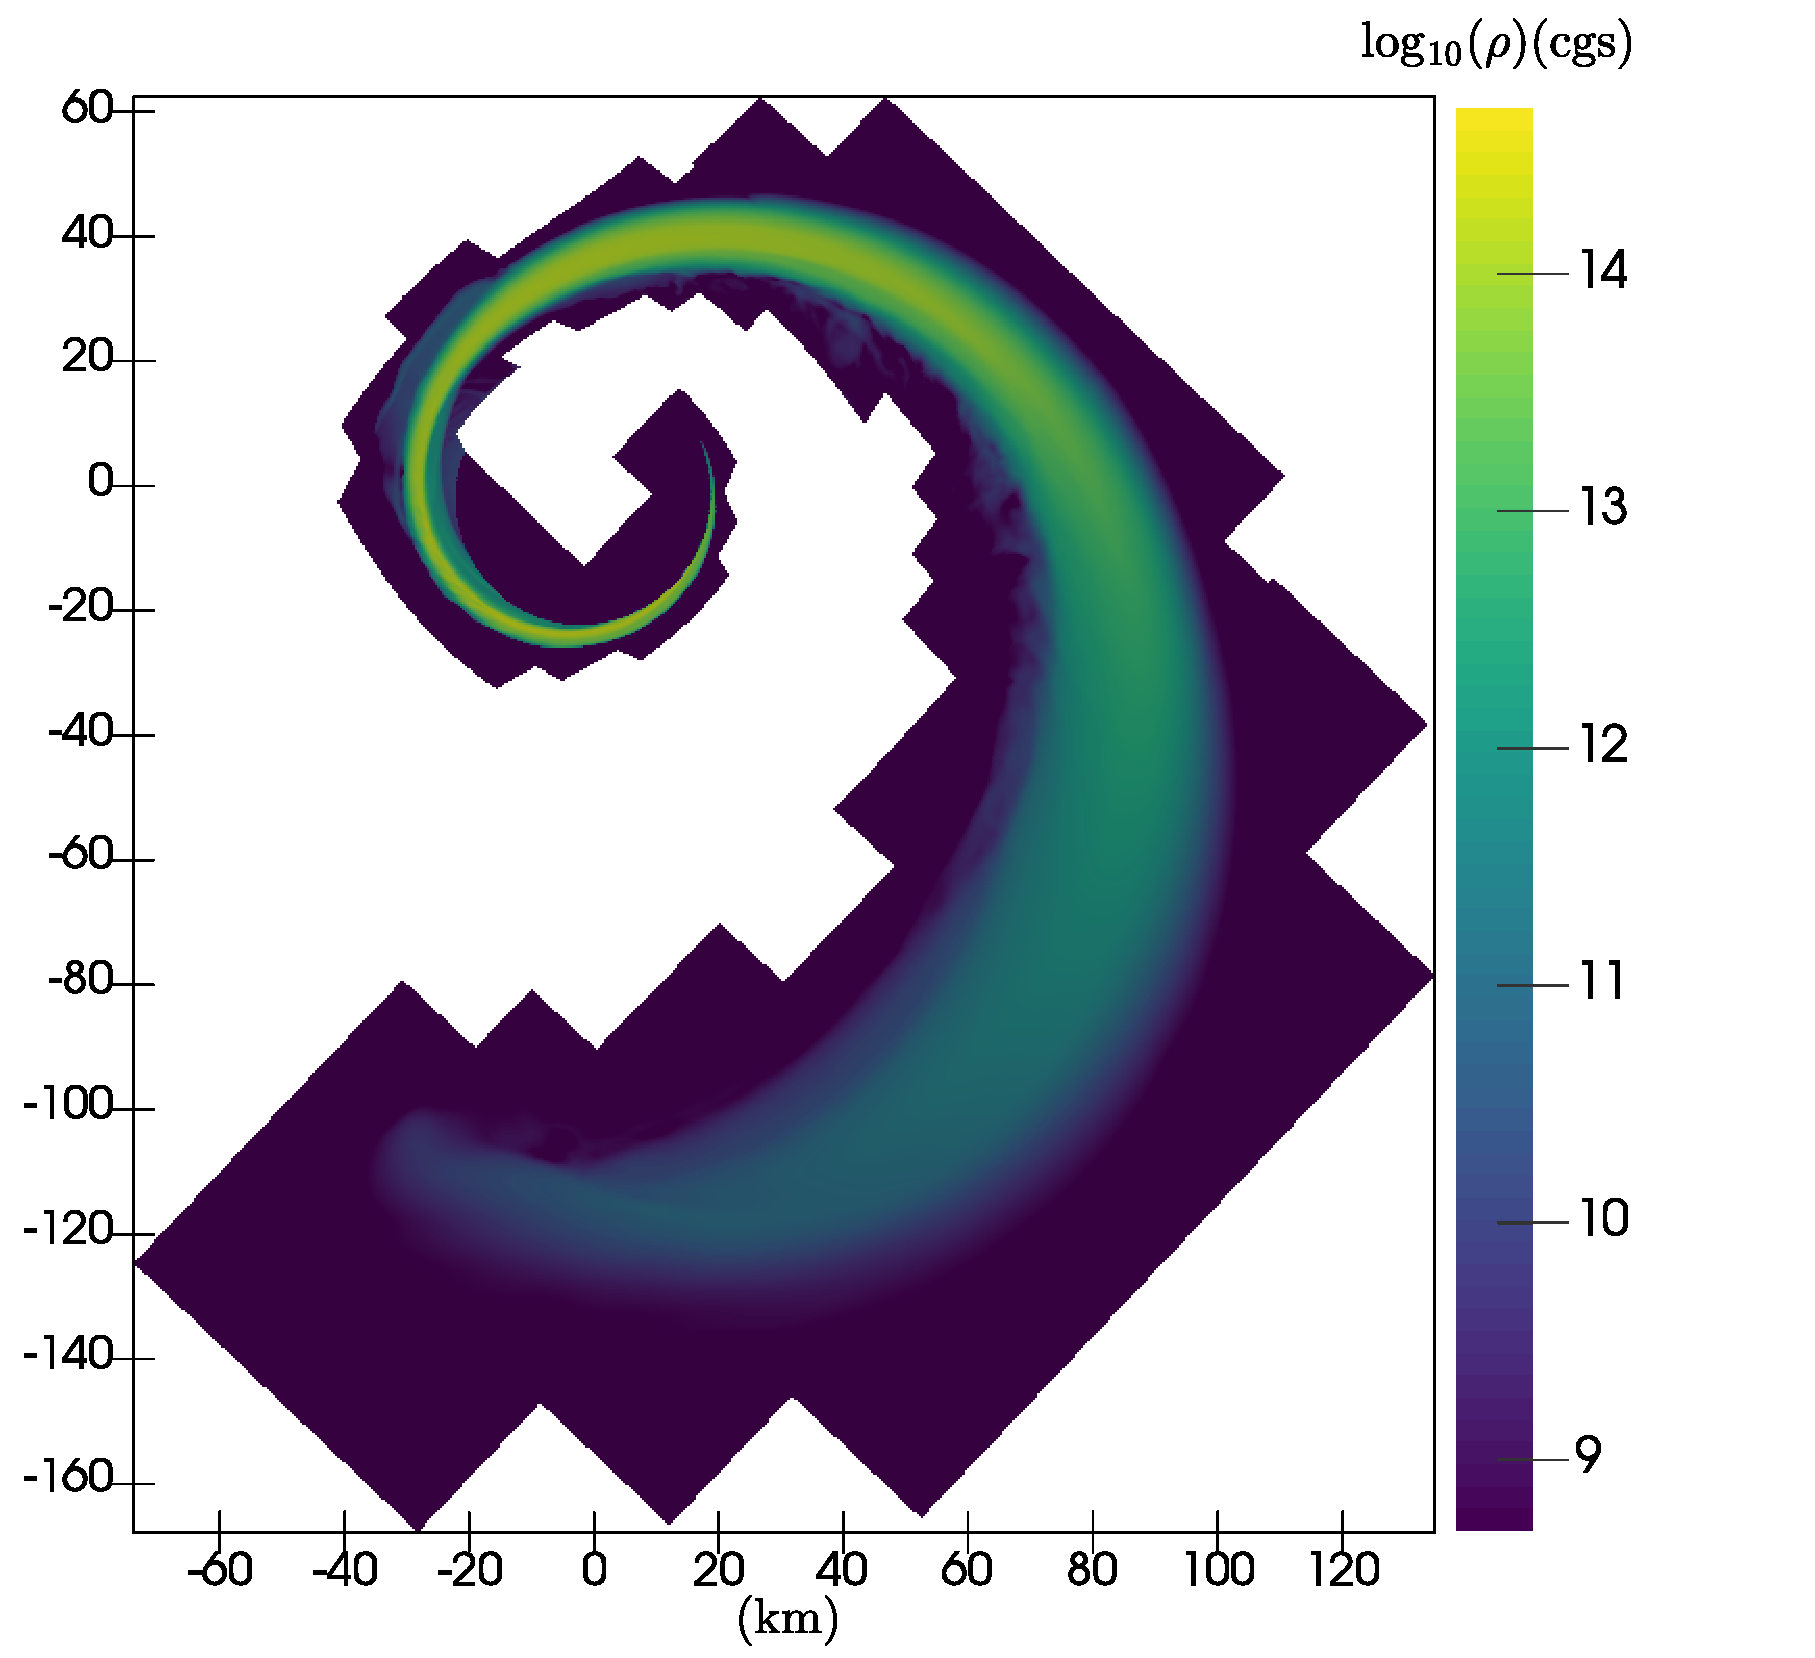
\includegraphics[width=1.0\linewidth]{images/rho_DD2_M12-merger-inertial}
		\label{fig:rho_M12_DD2}
	\end{subfigure}
	\begin{subfigure}[b]{0.475\textwidth}
		\centering
		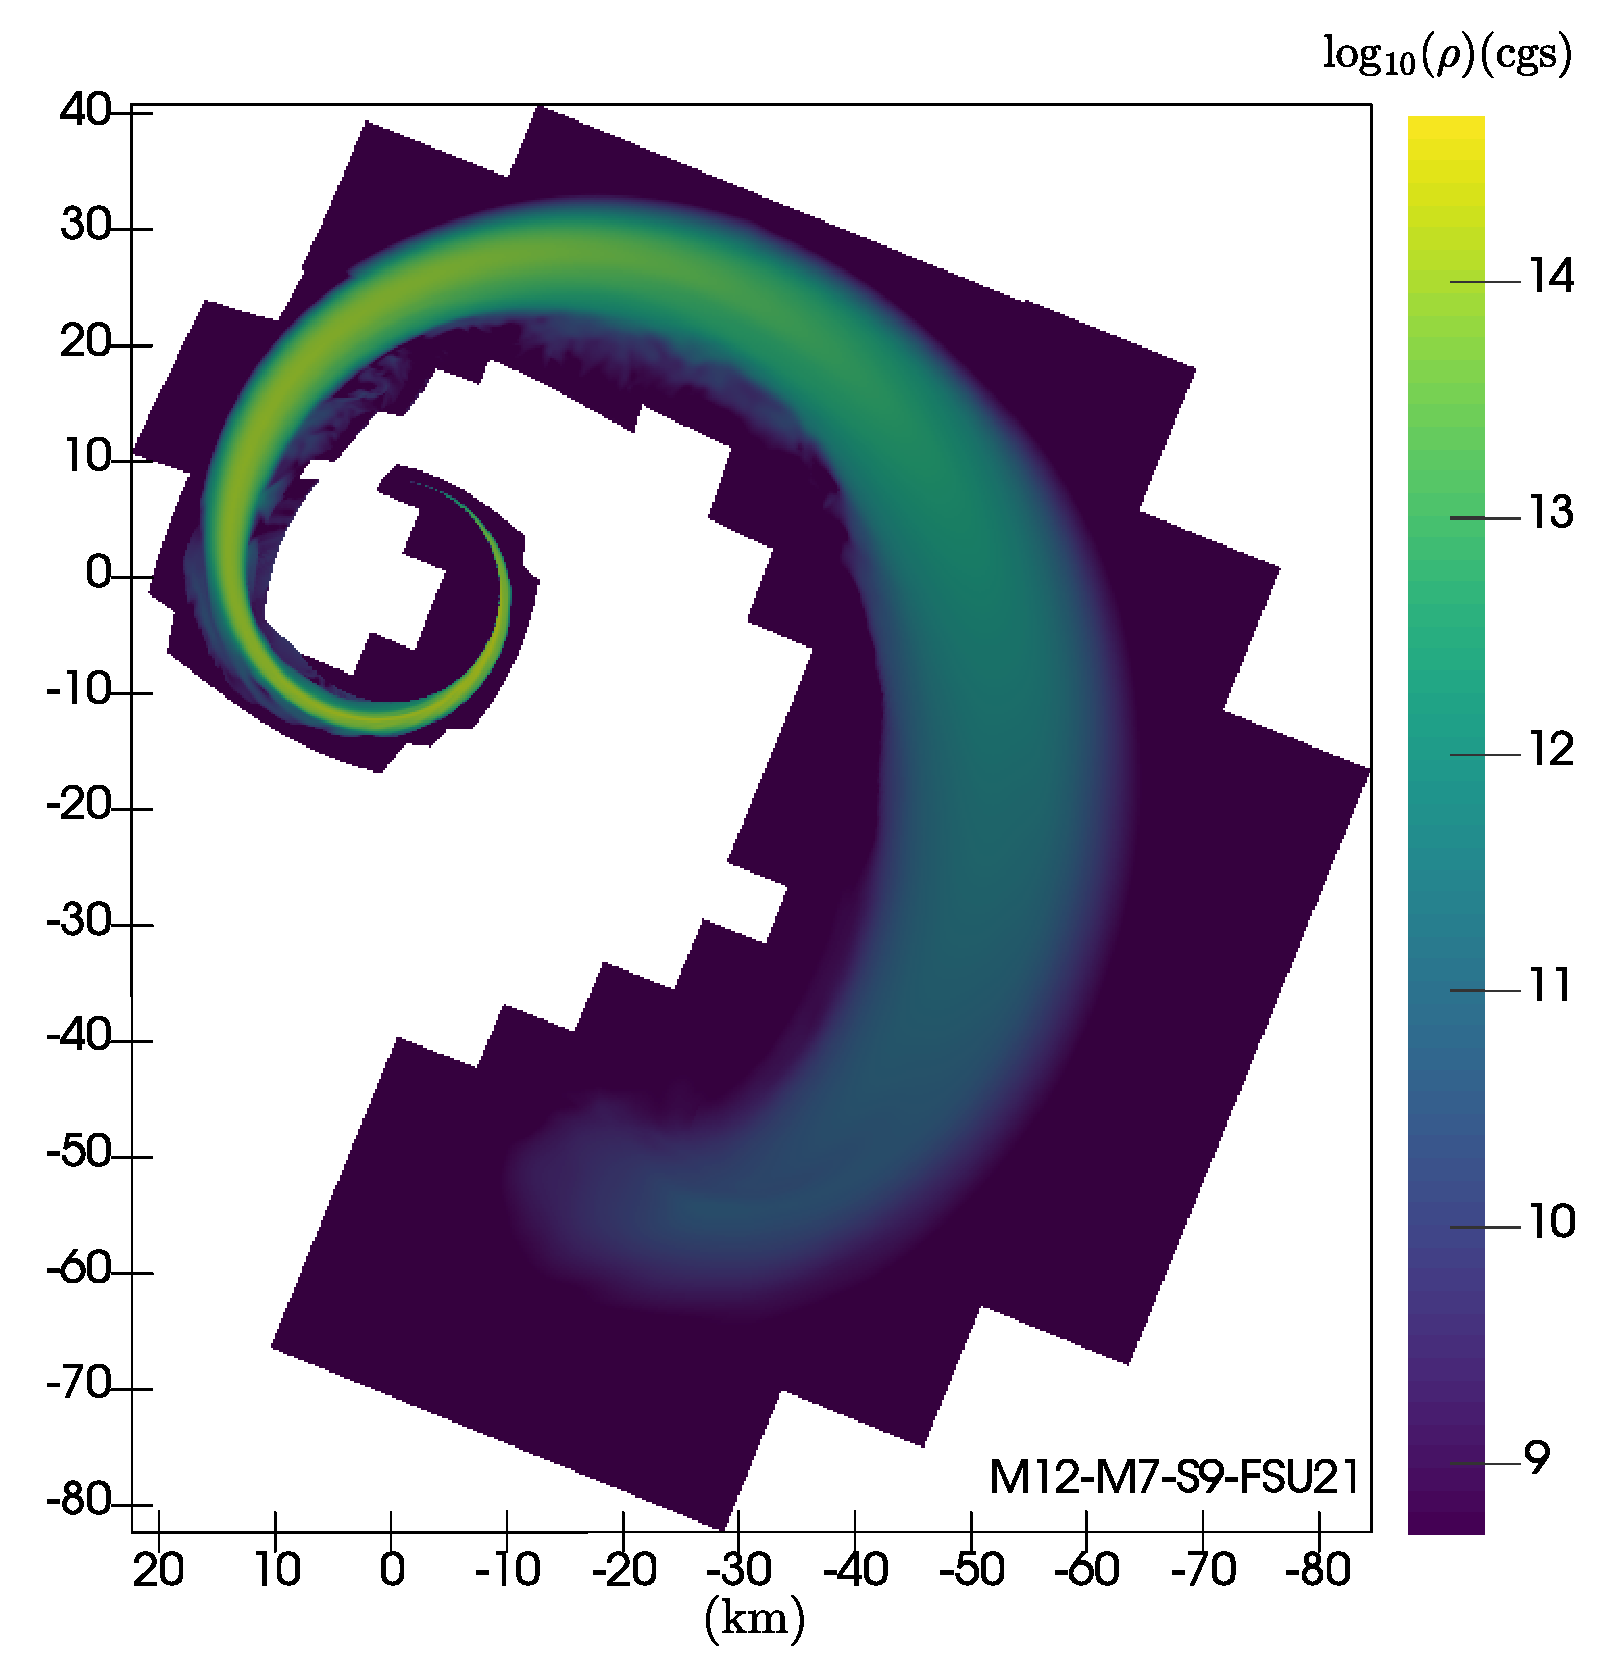
\includegraphics[width=\linewidth]{images/rho_FSU21_M12-merger-inertial}
		\label{fig:rho_M12_FSU21}
	\centering
	\end{subfigure}
	\begin{subfigure}[b]{0.475\textwidth}
		\centering
		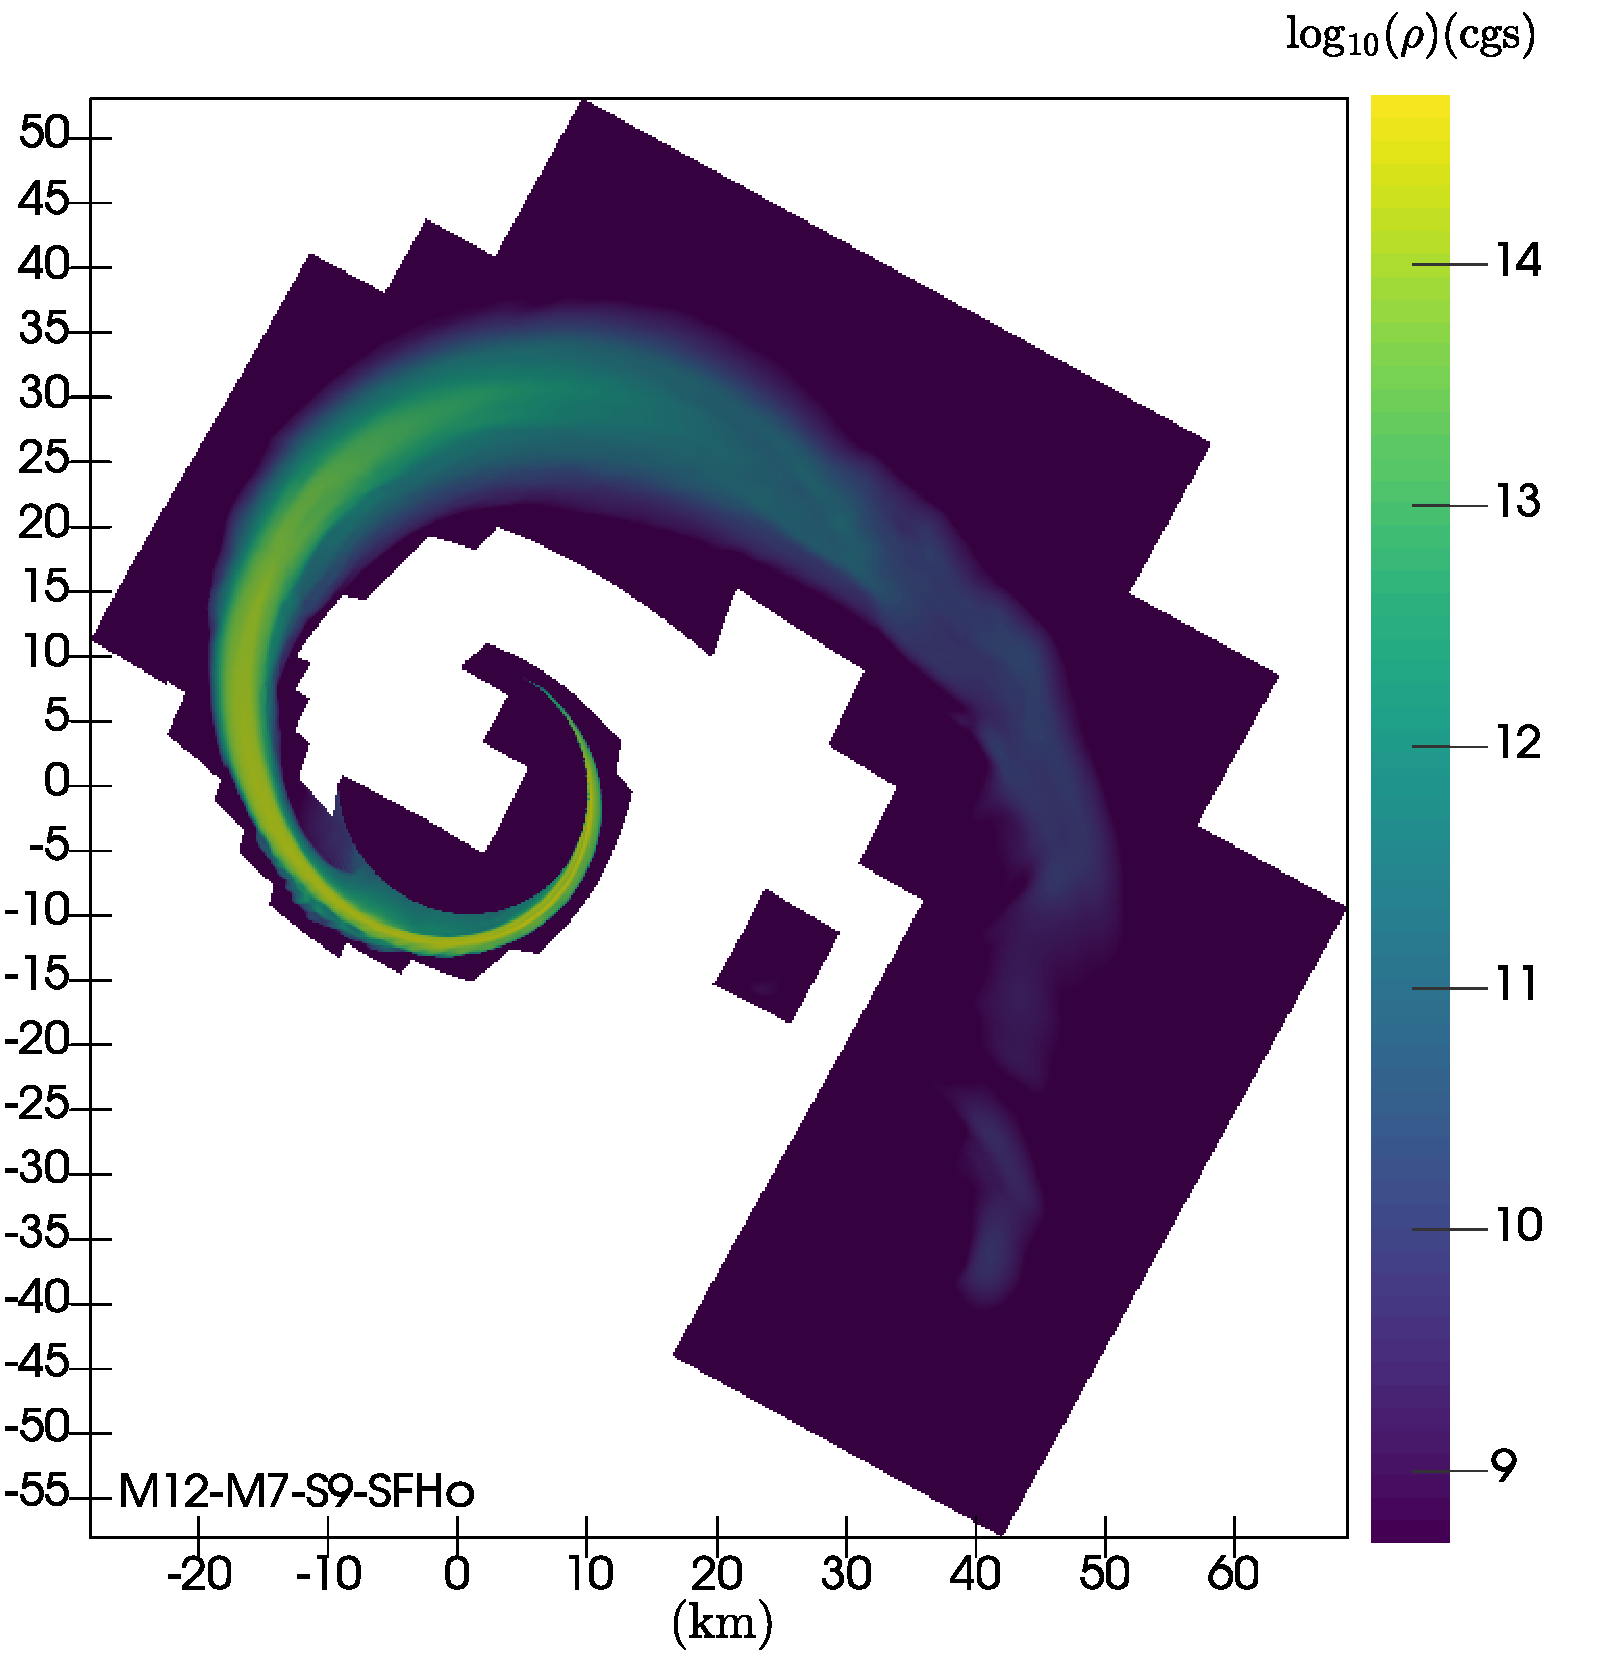
\includegraphics[width=\linewidth]{images/rho_SFHo_M12-merger-inertial}
		\label{fig:rho_M12_SFHo}
	\end{subfigure}
	\begin{subfigure}[b]{0.475\textwidth}
		\centering
		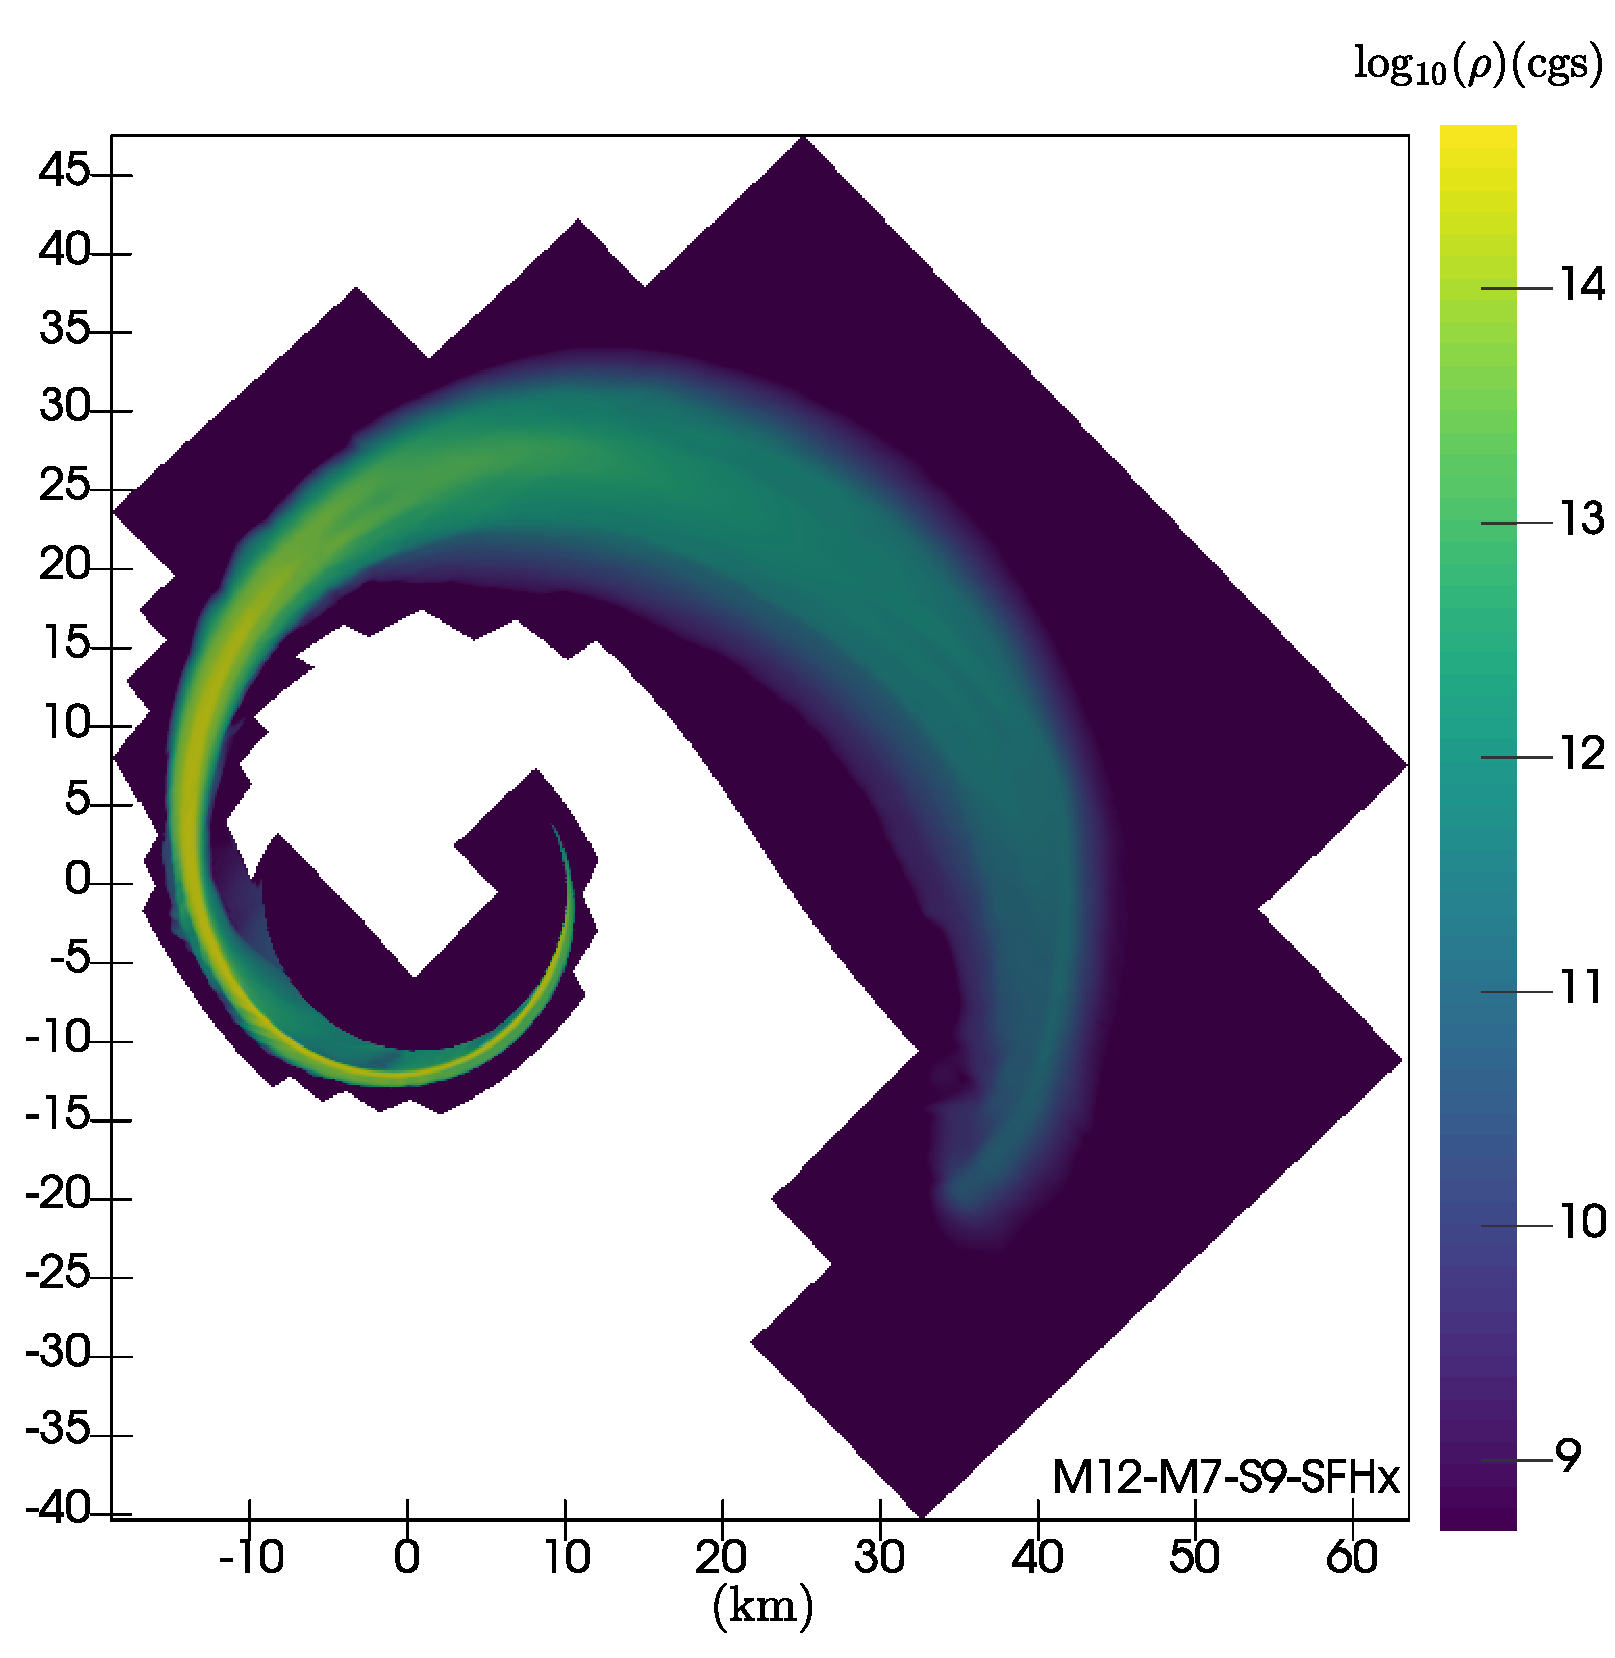
\includegraphics[width=\linewidth]{images/rho_SFHx_M12-merger-inertial}
		\label{fig:rho_M12_SFHx}
	\end{subfigure}
	\caption[Density profiles on equatorial plane for $1.2 M_{\odot}$ models]{
		Baryon density profiles on the equatorial plane for $M_{\rm NS} = 1.2 M_{\odot}$ models when $50\%$ of the neutron star material has been accreted onto the black hole.
		\textit{Top left:} Model M12-M7-S9-DD2.
		\textit{Top right:} Model M12-M7-S9-FSU21.
		\textit{Bottom left:} Model M12-M7-S9-SFHo.
		\textit{Bottom right:} Model M12-M7-S9-SFHx.
		White regions are not covered by the finite volume grid, while some fluid subdomains overlap the excised region of the black hole which can be seen near the interface of inflowing matter and the horizon.  We bracket the baryon density between $\sym \rho_{\rm FMR}$ and the fiducial density, $10^{14.7} {\rm g\,cm^{-3}}$. Note the distortion (and rotation) of the finite volume subdomain boundaries in the finest, innermost level, since the fluid is evolved in the coordinates of the (non-rotating) pseudo-spectral grid and we are viewing the systems in the inertial frame.  Also note the difference in length scales between models at merger time.
	}
	\label{fig:rho_M12}
\end{figure}

In Figure \ref{fig:rho_M12} we show the snapshot of each $1.2 M_\odot$ model on the equatorial plane when 50\% of the neutron star material has been accreted onto the black hole.  In Figure \ref{fig:rho_M14}, Model M14-M7-S9-FSU21 shows the poofiest, outer tail, measuring $\sym 20 {\rm km}$ across, while M12-M7-S9-DD2 measures at $\sym 12 {\rm km}$ in breadth.  The infalling stream near the horizon gets very narrow, and as such caused a number of our softest models to become too difficult to evolve.  Both SFHx as well as the M14-M7-S9-SFHo models did not proceed past merger beyond a few fractions of a millisecond.  

Consulting Figure \ref{fig:MultGammavsRho}, while all models soften near the fiducial density, the most drastic change in the high-density infalling region occurs in SFHx.  In our studies, the measured average temperature of the soft $1.4 M_\odot$ models was much higher near merger time (at which point the average temperature in all models reaches a maximum), and could indicate that the simulations were poorly resolved, at least in the innermost levels of the finite volume grid.  Therefore, we do not include the snapshots for M14-M7-S9-SFHo of M14-M7-S9-SFHx, while the snapshot for M12-M7-S9-SFHx is only included because it was well-behaved up to merger.

\begin{figure*}
	\centering
	\begin{subfigure}[b]{0.475\textwidth}
		\centering
		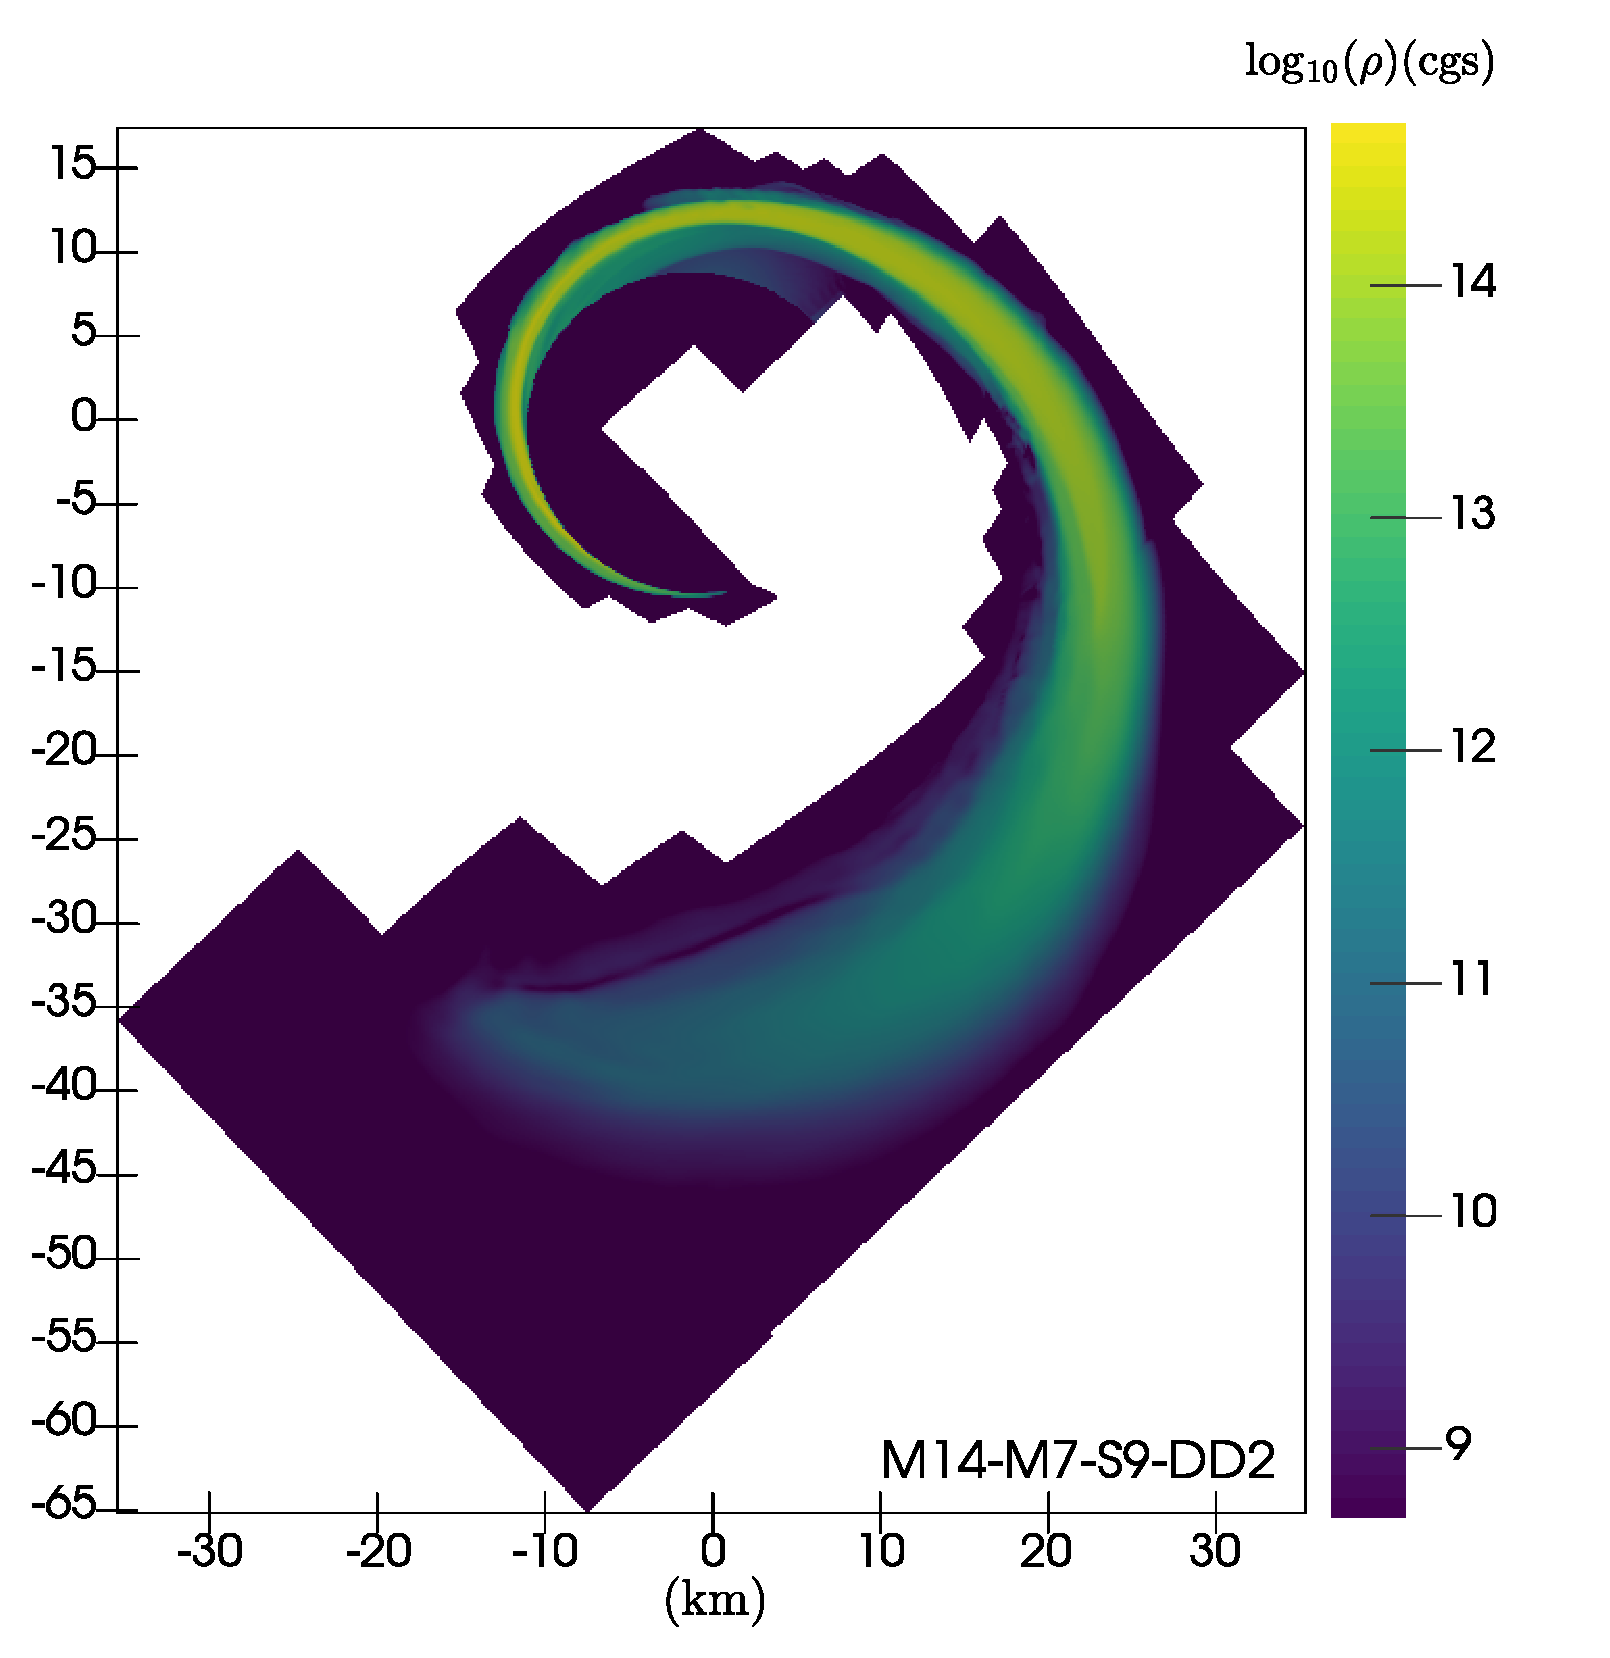
\includegraphics[width=1.0\linewidth]{images/rho_DD2_M14-merger-inertial}
		\label{fig:rho_M14_DD2}
	\end{subfigure}
	\begin{subfigure}[b]{0.475\textwidth}
		\centering
		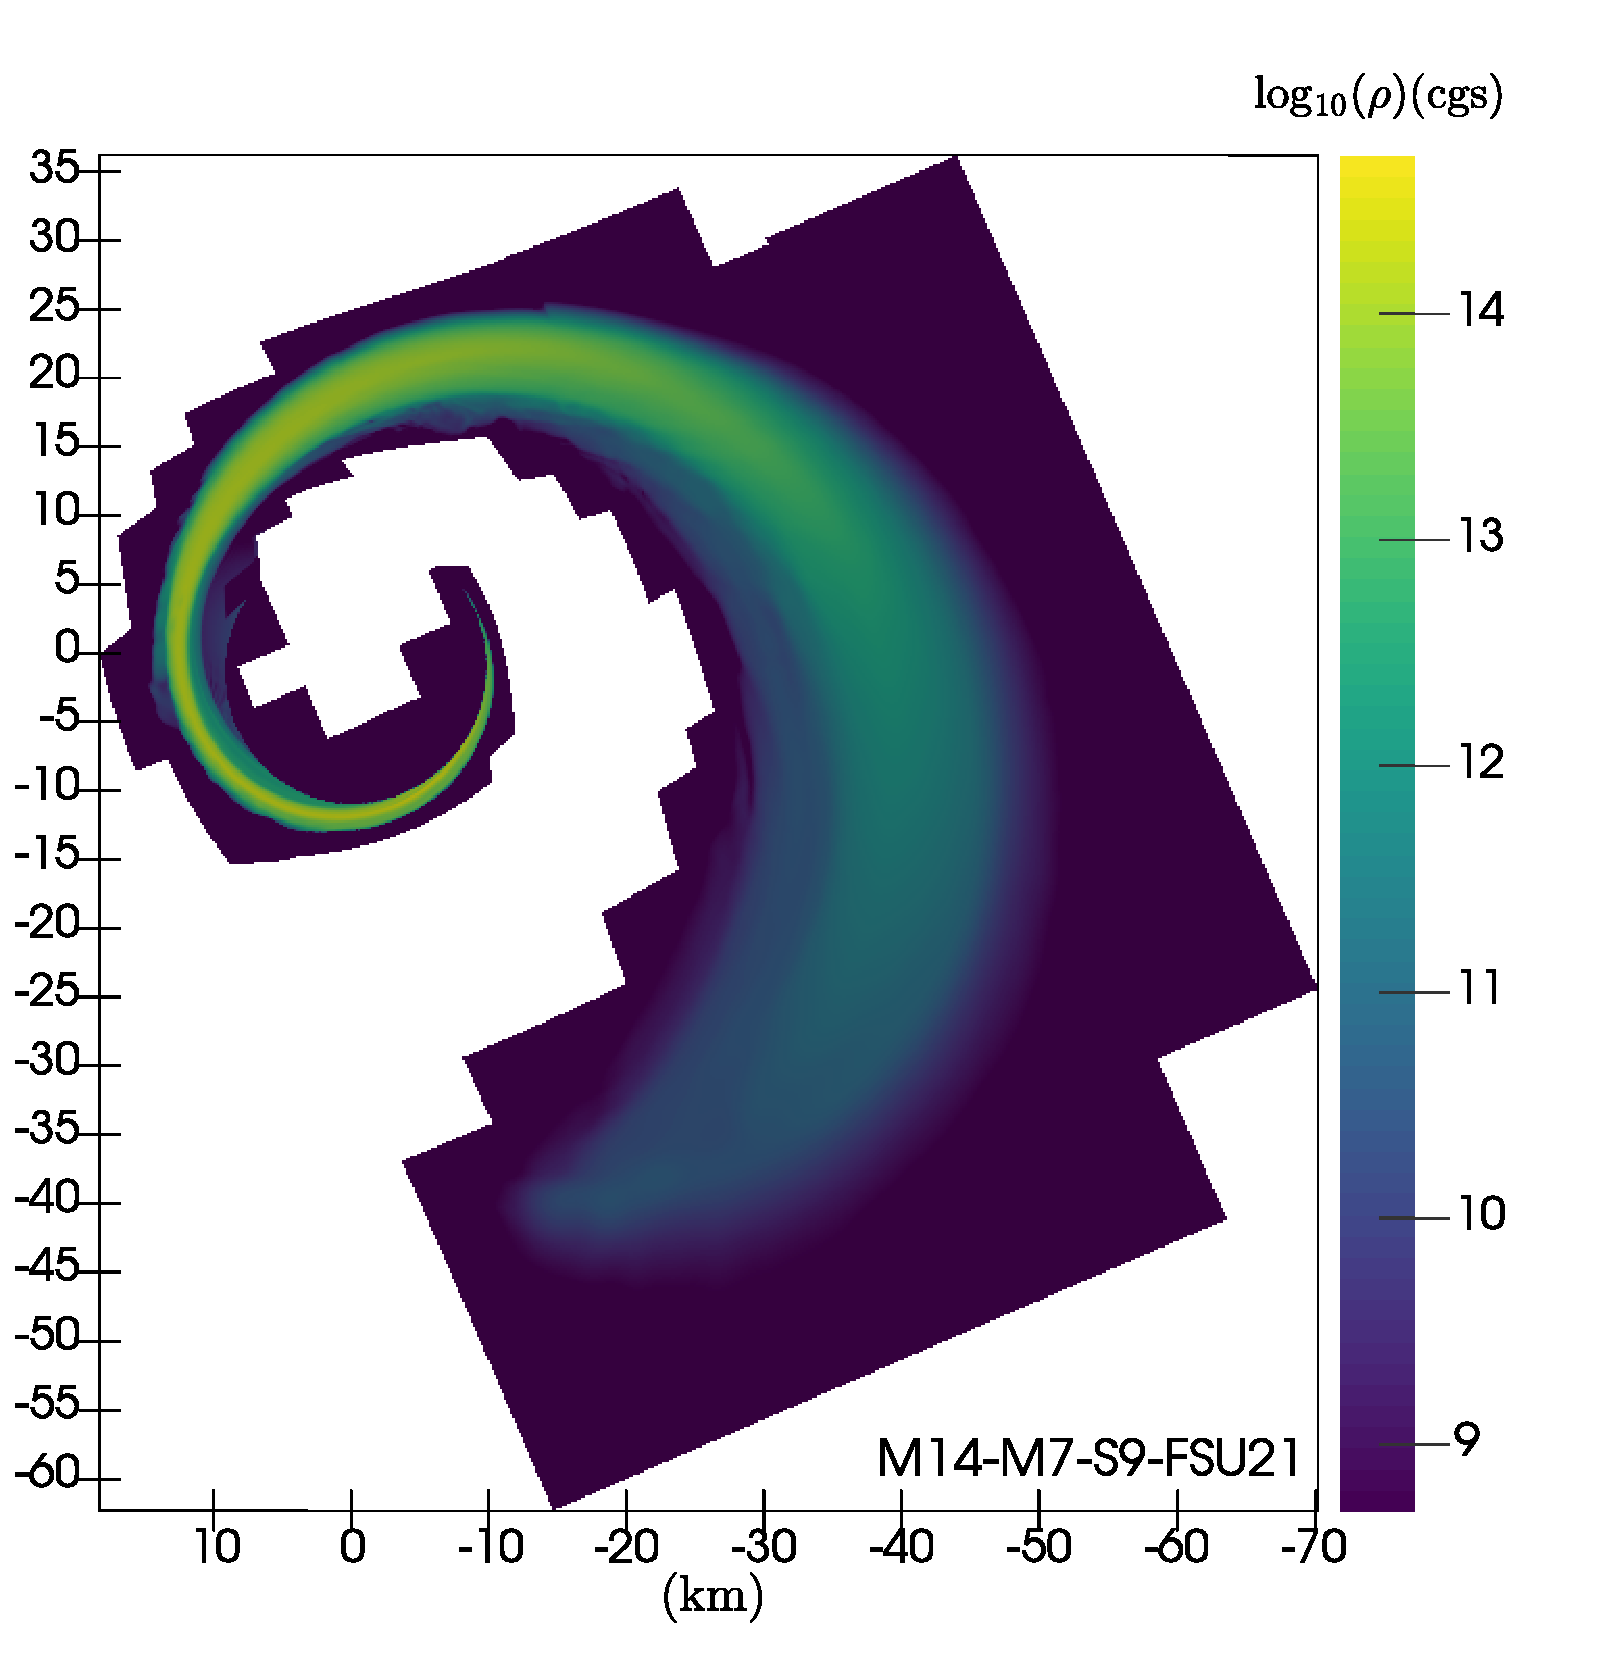
\includegraphics[width=\linewidth]{images/rho_FSU21_M14-merger-inertial}
		\label{fig:rho_M14_FSU21}
		\centering
	\end{subfigure}
	\caption[Density profiles on equatorial plane for $1.4 M_{\odot}$ models]{
	Baryon density profiles on the equatorial plane for $M_{\rm NS} = 1.4 M_{\odot}$ models when $50\%$ of the neutron star material has been accreted onto the black hole.
	\textit{Left:} Model M14-M7-S9-DD2.
	\textit{Right:} Model M14-M7-S9-FSU21.
	To add to the caption in Figure \ref{fig:rho_M12}, we note that the FSU2.1 profiles are represented with a $90^{\circ}$ counterclockwise rotation in the inertial frame.  This is done for sake of maintaining a similar aspect ratio to the others.  Note that FSU2.1 had the fewest number of orbits in our simulations (see Table \ref{tab:id}). 
	}
	\label{fig:rho_M14}
\end{figure*}

Shortly after the merger, between the time of merger and the first local minimum of the accretion rate and average temperature, we derefine the innermost finite volume level by a factor of two.
The fluid begins to circularize $\sym (3-4) {\rm ms}$ after merger in all models.
We perform a second derefinement by a factor of two more at 
this stage as well, since the material becomes less dense and easier to resolve.



\begin{table}
	\begin{center}
		\caption[Properties of the dynamical ejecta and post merger remnant]{
			Properties of the dynamical ejecta and post merger remnant. $M_{\rm BH}^f$ and  $\chi_{\rm BH}^f$  are the mass and dimensionless spin of the black hole,
			and $M_{\rm out}^f$ is the baryon mass remaining outside of the black hole. Those quantities are measured at the first minima of the accretion rate onto the black hole,
			before circularization of the accretion disk. The baryon mass outside of the black hole immediately after disk formation (which is a more vaguely defined
			time) is typically $10\%-20\%$ lower than $M_{\rm out}^f$. $M_{\rm ej}$ is the mass of the dynamical ejecta, and $\langle v/c\rangle_{\rm ej}$. All these properties are nearly constant, from about $1\,{\rm ms}$ after the merger. Bracketed numbers for
			$M_{\rm out}^f$ and $M_{\rm ej}$ show semi-analytical predictions for the mass outside of the black hole $10\,{\rm ms}$ after merger~\cite{Foucart2012},
			and the ejected mass~\cite{Kawaguchi:2016}, while bracketed numbers for $M_{\rm BH}^f$ and $\chi_{\rm BH}^f$ are semi-analytical predictions
			from~\cite{Pannarale:2014}. Those values were calculated from the equations in~\cite{Pannarale:2014} using a root-finding code for both the innermost stable spherical orbit and the reported quantities.  Relative errors in the determination of $M_{\rm ej}$ are $\sim 20\%$, the black holes properties are
			accurate to $\sim 1\%$, and other quantities have relative errors of $\sim 10\%$.
		}
		\label{tab:results}
		{
			\begin{tabular}{c cc ccc}
	\toprule \toprule
	Model & $M_{\rm BH}^f\,(M_\odot)$ & $\chi_{\rm BH}^f$ & $M_{\rm out}^f\,(10^{-2} M_\odot)$ & $M_{\rm ej}\,(10^{-2} M_\odot)$ & $\langle v/c \rangle_{\rm ej}$\\
	\midrule
	M12-M7-S9-DD2 & -- [7.7] & -- [0.93] & -- [36] & 7.2 [7.2] & 0.21\\
	M14-M7-S9-DD2 & -- [7.9] & -- [0.93] & -- [34] & 6.0 [3.6] & 0.20\\
	M12-M7-S9-FSU21 & -- [7.7] & -- [0.93] & -- [38] & 7.8 [10.7] & 0.20\\
	M14-M7-S9-FSU21 & -- [7.9] & -- [0.93] & -- [36] & 5.9 [6.4] & 0.19\\
	M12-M7-S9-SFHo & -- [7.8] & -- [0.93] & -- [30] & $\sym 3.8$ [4.3] & $\sym 0.18$\\
	M14-M7-S9-SFHo & -- [8.0] & -- [0.93] & -- [26] & -- [2.3] & --\\
	M12-M7-S9-SFHx & -- [7.8] & -- [0.93] & -- [30] & $\sym 5.7$ [5.9] & $\sym0.20 $\\
	M14-M7-S9-SFHx & -- [8.0] & -- [0.93] & -- [26] & -- [2.6] & --\\
%	M12-M7-S9-LS220 & -- [7.8] & -- [0.93] & -- [34] & -- [9.4] & --\\
%	M14-M7-S9-LS220 & -- [8.0] & -- [0.93] & -- [31] & -- [4.7] & --\\
	\bottomrule \bottomrule
\end{tabular}
		}
	\end{center}
\end{table}



\section{Outflow analysis: properties of the ejecta}
\label{sec:tail-analysis}

In this section, we consider the ejecta that results from the tidal disruption of the neutron star, leaving aside the second source of late-stage ejecta which occurs via neutrino driven winds and magnetic effects in accretion disk outlfows.  As our models do not incorporate magnetohydrodynamics and since we only implement a simple leakage scheme to approximately capture the effects of neutrino cooling on the post-merger remnant of Section \ref{sec:disk-analysis}, we do not evolve the remaining models beyond $10 {\rm ms}$ passed the onset of merger.

For those models that evolved out to $5 {\rm ms}$ passed merger, we find that at that time, the ejecta mass $M_{\rm ej}$ is roughly constrained between $\sym (4 - 8) \times 10^{-2} M_\odot$.
In table \ref{tab:results}, we display our measured results at $5 {\rm ms}$ after measure compared to the predicted results from the fitting formulae.  
As described by the fitting formulae, the stiffer, finite-temperature equations of state do indeed disrupt further outside the ISCO, while the softer one disrupts much closer and results in more interaction between the protodisk and the fallback material.


\begin{figure}
	\centering
	% GNUPLOT: LaTeX picture with Postscript
\begingroup
  \makeatletter
  \providecommand\color[2][]{%
    \GenericError{(gnuplot) \space\space\space\@spaces}{%
      Package color not loaded in conjunction with
      terminal option `colourtext'%
    }{See the gnuplot documentation for explanation.%
    }{Either use 'blacktext' in gnuplot or load the package
      color.sty in LaTeX.}%
    \renewcommand\color[2][]{}%
  }%
  \providecommand\includegraphics[2][]{%
    \GenericError{(gnuplot) \space\space\space\@spaces}{%
      Package graphicx or graphics not loaded%
    }{See the gnuplot documentation for explanation.%
    }{The gnuplot epslatex terminal needs graphicx.sty or graphics.sty.}%
    \renewcommand\includegraphics[2][]{}%
  }%
  \providecommand\rotatebox[2]{#2}%
  \@ifundefined{ifGPcolor}{%
    \newif\ifGPcolor
    \GPcolortrue
  }{}%
  \@ifundefined{ifGPblacktext}{%
    \newif\ifGPblacktext
    \GPblacktexttrue
  }{}%
  % define a \g@addto@macro without @ in the name:
  \let\gplgaddtomacro\g@addto@macro
  % define empty templates for all commands taking text:
  \gdef\gplbacktext{}%
  \gdef\gplfronttext{}%
  \makeatother
  \ifGPblacktext
    % no textcolor at all
    \def\colorrgb#1{}%
    \def\colorgray#1{}%
  \else
    % gray or color?
    \ifGPcolor
      \def\colorrgb#1{\color[rgb]{#1}}%
      \def\colorgray#1{\color[gray]{#1}}%
      \expandafter\def\csname LTw\endcsname{\color{white}}%
      \expandafter\def\csname LTb\endcsname{\color{black}}%
      \expandafter\def\csname LTa\endcsname{\color{black}}%
      \expandafter\def\csname LT0\endcsname{\color[rgb]{1,0,0}}%
      \expandafter\def\csname LT1\endcsname{\color[rgb]{0,1,0}}%
      \expandafter\def\csname LT2\endcsname{\color[rgb]{0,0,1}}%
      \expandafter\def\csname LT3\endcsname{\color[rgb]{1,0,1}}%
      \expandafter\def\csname LT4\endcsname{\color[rgb]{0,1,1}}%
      \expandafter\def\csname LT5\endcsname{\color[rgb]{1,1,0}}%
      \expandafter\def\csname LT6\endcsname{\color[rgb]{0,0,0}}%
      \expandafter\def\csname LT7\endcsname{\color[rgb]{1,0.3,0}}%
      \expandafter\def\csname LT8\endcsname{\color[rgb]{0.5,0.5,0.5}}%
    \else
      % gray
      \def\colorrgb#1{\color{black}}%
      \def\colorgray#1{\color[gray]{#1}}%
      \expandafter\def\csname LTw\endcsname{\color{white}}%
      \expandafter\def\csname LTb\endcsname{\color{black}}%
      \expandafter\def\csname LTa\endcsname{\color{black}}%
      \expandafter\def\csname LT0\endcsname{\color{black}}%
      \expandafter\def\csname LT1\endcsname{\color{black}}%
      \expandafter\def\csname LT2\endcsname{\color{black}}%
      \expandafter\def\csname LT3\endcsname{\color{black}}%
      \expandafter\def\csname LT4\endcsname{\color{black}}%
      \expandafter\def\csname LT5\endcsname{\color{black}}%
      \expandafter\def\csname LT6\endcsname{\color{black}}%
      \expandafter\def\csname LT7\endcsname{\color{black}}%
      \expandafter\def\csname LT8\endcsname{\color{black}}%
    \fi
  \fi
  \setlength{\unitlength}{0.0500bp}%
  \begin{picture}(7920.00,5040.00)%
    \gplgaddtomacro\gplbacktext{%
      \csname LTb\endcsname%
      \put(1342,704){\makebox(0,0)[r]{\strut{} 1e-07}}%
      \put(1342,1383){\makebox(0,0)[r]{\strut{} 1e-06}}%
      \put(1342,2061){\makebox(0,0)[r]{\strut{} 1e-05}}%
      \put(1342,2740){\makebox(0,0)[r]{\strut{} 0.0001}}%
      \put(1342,3418){\makebox(0,0)[r]{\strut{} 0.001}}%
      \put(1342,4097){\makebox(0,0)[r]{\strut{} 0.01}}%
      \put(1342,4775){\makebox(0,0)[r]{\strut{} 0.1}}%
      \put(1474,484){\makebox(0,0){\strut{} 0}}%
      \put(2684,484){\makebox(0,0){\strut{} 0.05}}%
      \put(3894,484){\makebox(0,0){\strut{} 0.1}}%
      \put(5103,484){\makebox(0,0){\strut{} 0.15}}%
      \put(6313,484){\makebox(0,0){\strut{} 0.2}}%
      \put(7523,484){\makebox(0,0){\strut{} 0.25}}%
      \put(176,2739){\rotatebox{-270}{\makebox(0,0){\strut{}$\log_{10}(M_{\rm ej})$ ($M_{\odot}$)}}}%
      \put(4498,154){\makebox(0,0){\strut{}$ Y_e $}}%
    }%
    \gplgaddtomacro\gplfronttext{%
      \csname LTb\endcsname%
      \put(6536,4602){\makebox(0,0)[r]{\strut{}M12-M7-S9-DD2}}%
      \csname LTb\endcsname%
      \put(6536,4382){\makebox(0,0)[r]{\strut{}M14-M7-S9-DD2}}%
      \csname LTb\endcsname%
      \put(6536,4162){\makebox(0,0)[r]{\strut{}M12-M7-S9-FSU21}}%
      \csname LTb\endcsname%
      \put(6536,3942){\makebox(0,0)[r]{\strut{}M14-M7-S9-FSU21}}%
      \csname LTb\endcsname%
      \put(6536,3722){\makebox(0,0)[r]{\strut{}M12-M7-S9-SFHo}}%
    }%
    \gplbacktext
    \put(0,0){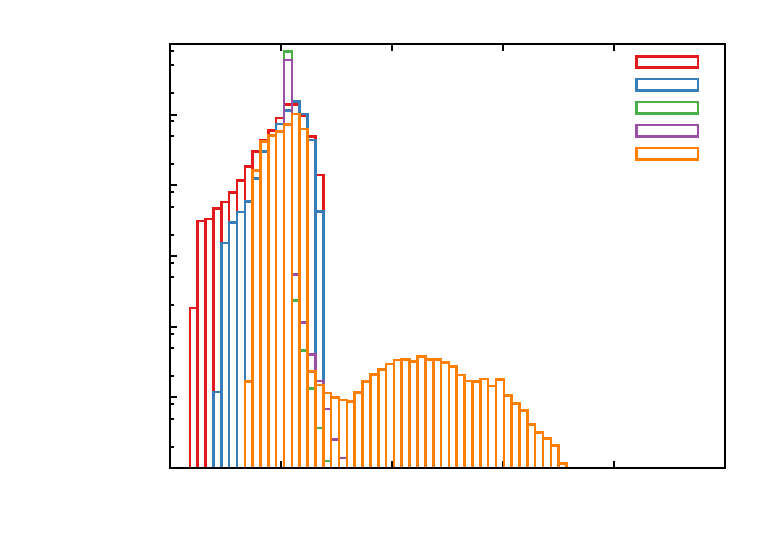
\includegraphics{images/unbound-mass-vs-Ye}}%
    \gplfronttext
  \end{picture}%
\endgroup

	\caption[Composition of the ejecta]{
		Electron fraction $Y_e$ of the ejecta measured 5 ms after merger.  We note that all of the matter peaks in the $Y_e \sym 0.05$ range, where M12-M7-S9-DD2 has the largest electron fraction range ($0.011 - 0.07$) while neither FSU21 models produce ejecta with $Y_e < 0.05$. ( FSU2.1 does not allow for $Y_e < 0.05$.  See Section \ref{sec:fsu21} and ~\cite{shen2011second}).
	}
	\label{fig:Yehisto}
\end{figure}

As in previous simulations of black hole-neutron star mergers, the ejecta in our models is very neutron rich, with a density-weighted average electron fraction of $Y_e \sim 0.05$).  
In Figure \ref{fig:Yehisto}, we show the (logarithmic) distribution of matter over the chemical composition in the unbound material.  
Most of the ejecta has $Y_e < 0.7$ while none of it has $Y_e > 0.25$ --- where lighter r-process elements might be produced.
Therefore, r-process nucleosynthesis will produce 2nd and 3rd peak heavy elements in the ejecta, with little production of light elements in the 1st peak.  
The unbound material will be very opaque, leading to an electromagnetic transient to peak in the infrared by the r-process ~\cite{2013ApJ...775...18B}.

\begin{figure}
	\centering
	% GNUPLOT: LaTeX picture with Postscript
\begingroup
  \makeatletter
  \providecommand\color[2][]{%
    \GenericError{(gnuplot) \space\space\space\@spaces}{%
      Package color not loaded in conjunction with
      terminal option `colourtext'%
    }{See the gnuplot documentation for explanation.%
    }{Either use 'blacktext' in gnuplot or load the package
      color.sty in LaTeX.}%
    \renewcommand\color[2][]{}%
  }%
  \providecommand\includegraphics[2][]{%
    \GenericError{(gnuplot) \space\space\space\@spaces}{%
      Package graphicx or graphics not loaded%
    }{See the gnuplot documentation for explanation.%
    }{The gnuplot epslatex terminal needs graphicx.sty or graphics.sty.}%
    \renewcommand\includegraphics[2][]{}%
  }%
  \providecommand\rotatebox[2]{#2}%
  \@ifundefined{ifGPcolor}{%
    \newif\ifGPcolor
    \GPcolortrue
  }{}%
  \@ifundefined{ifGPblacktext}{%
    \newif\ifGPblacktext
    \GPblacktexttrue
  }{}%
  % define a \g@addto@macro without @ in the name:
  \let\gplgaddtomacro\g@addto@macro
  % define empty templates for all commands taking text:
  \gdef\gplbacktext{}%
  \gdef\gplfronttext{}%
  \makeatother
  \ifGPblacktext
    % no textcolor at all
    \def\colorrgb#1{}%
    \def\colorgray#1{}%
  \else
    % gray or color?
    \ifGPcolor
      \def\colorrgb#1{\color[rgb]{#1}}%
      \def\colorgray#1{\color[gray]{#1}}%
      \expandafter\def\csname LTw\endcsname{\color{white}}%
      \expandafter\def\csname LTb\endcsname{\color{black}}%
      \expandafter\def\csname LTa\endcsname{\color{black}}%
      \expandafter\def\csname LT0\endcsname{\color[rgb]{1,0,0}}%
      \expandafter\def\csname LT1\endcsname{\color[rgb]{0,1,0}}%
      \expandafter\def\csname LT2\endcsname{\color[rgb]{0,0,1}}%
      \expandafter\def\csname LT3\endcsname{\color[rgb]{1,0,1}}%
      \expandafter\def\csname LT4\endcsname{\color[rgb]{0,1,1}}%
      \expandafter\def\csname LT5\endcsname{\color[rgb]{1,1,0}}%
      \expandafter\def\csname LT6\endcsname{\color[rgb]{0,0,0}}%
      \expandafter\def\csname LT7\endcsname{\color[rgb]{1,0.3,0}}%
      \expandafter\def\csname LT8\endcsname{\color[rgb]{0.5,0.5,0.5}}%
    \else
      % gray
      \def\colorrgb#1{\color{black}}%
      \def\colorgray#1{\color[gray]{#1}}%
      \expandafter\def\csname LTw\endcsname{\color{white}}%
      \expandafter\def\csname LTb\endcsname{\color{black}}%
      \expandafter\def\csname LTa\endcsname{\color{black}}%
      \expandafter\def\csname LT0\endcsname{\color{black}}%
      \expandafter\def\csname LT1\endcsname{\color{black}}%
      \expandafter\def\csname LT2\endcsname{\color{black}}%
      \expandafter\def\csname LT3\endcsname{\color{black}}%
      \expandafter\def\csname LT4\endcsname{\color{black}}%
      \expandafter\def\csname LT5\endcsname{\color{black}}%
      \expandafter\def\csname LT6\endcsname{\color{black}}%
      \expandafter\def\csname LT7\endcsname{\color{black}}%
      \expandafter\def\csname LT8\endcsname{\color{black}}%
    \fi
  \fi
  \setlength{\unitlength}{0.0500bp}%
  \begin{picture}(7920.00,5040.00)%
    \gplgaddtomacro\gplbacktext{%
      \csname LTb\endcsname%
      \put(1210,704){\makebox(0,0)[r]{\strut{} 0}}%
      \put(1210,1609){\makebox(0,0)[r]{\strut{} 0.001}}%
      \put(1210,2513){\makebox(0,0)[r]{\strut{} 0.002}}%
      \put(1210,3418){\makebox(0,0)[r]{\strut{} 0.003}}%
      \put(1210,4323){\makebox(0,0)[r]{\strut{} 0.004}}%
      \put(1342,484){\makebox(0,0){\strut{} 0}}%
      \put(2578,484){\makebox(0,0){\strut{} 0.1}}%
      \put(3814,484){\makebox(0,0){\strut{} 0.2}}%
      \put(5051,484){\makebox(0,0){\strut{} 0.3}}%
      \put(6287,484){\makebox(0,0){\strut{} 0.4}}%
      \put(7523,484){\makebox(0,0){\strut{} 0.5}}%
      \put(176,2739){\rotatebox{-270}{\makebox(0,0){\strut{}$M_{\rm ej}$ ($M_{\odot}$)}}}%
      \put(4432,154){\makebox(0,0){\strut{}$ v_r/c $}}%
    }%
    \gplgaddtomacro\gplfronttext{%
      \csname LTb\endcsname%
      \put(6536,4602){\makebox(0,0)[r]{\strut{}M12-M7-S9-DD2}}%
      \csname LTb\endcsname%
      \put(6536,4382){\makebox(0,0)[r]{\strut{}M14-M7-S9-DD2}}%
      \csname LTb\endcsname%
      \put(6536,4162){\makebox(0,0)[r]{\strut{}M12-M7-S9-FSU21}}%
      \csname LTb\endcsname%
      \put(6536,3942){\makebox(0,0)[r]{\strut{}M14-M7-S9-FSU21}}%
      \csname LTb\endcsname%
      \put(6536,3722){\makebox(0,0)[r]{\strut{}M12-M7-S9-SFHo}}%
    }%
    \gplbacktext
    \put(0,0){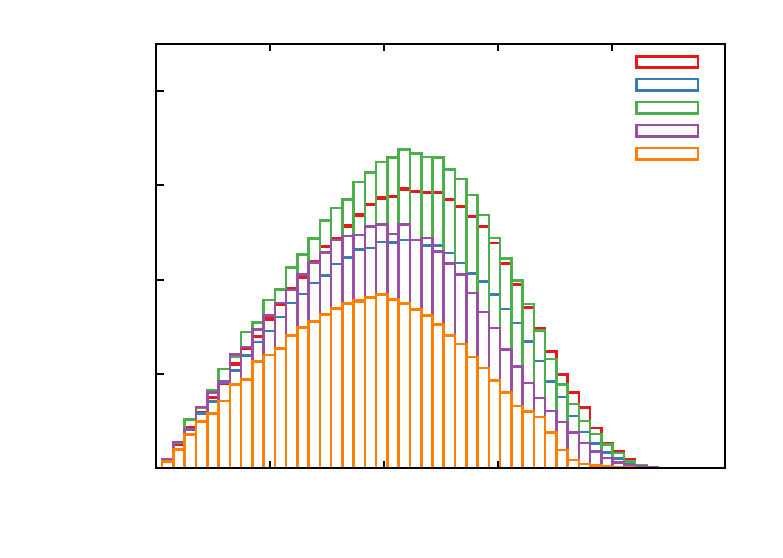
\includegraphics{images/unbound-mass-vs-Vinf}}%
    \gplfronttext
  \end{picture}%
\endgroup

	\caption[Distribution of the asymptotic velocity of the ejecta]{
		Distribution of the asymptotic velocity of the ejecta measured 5 ms after merger.
	}
	\label{fig:vrhisto}
\end{figure}

We can also determine information about the infrared transient from the asymptotic velocity of the ejecta.  
Since greater velocities lead to faster expansion of the unbound material, the transient will be be shorter lived and have a larger amplitude~\cite{2013ApJ...775...18B,Barnes:2016}. 
In Figure \ref{fig:vrhisto}, the distribution of the ejecta velocities peak around $\langle v \rangle \sim 0.2 c$, with a broad distribution  $ 0 \le v \le 2 \langle v \rangle $.
Model M12-M7-S9-SFHo clearly has the least amount of ejecta.

The average kinetic energy of the ejecta was measured to lie between $3.7 \times 10^{52} {\rm ergs} $ for the SFHo model and $4.8 \times 10^{52} {\rm ergs} $ for the M12-M7-S9-DD2 model.  
The $1.4 M_\odot$ models had energies inside this range. 
The ejecta steadily cools within 1 ms after merger with to a steady temperature in the range of $T \sim (0.1 - 0.4) {\rm MeV}$, bounded by both FSU2.1 models in the higher range and the remaining models in the lower range.

\begin{figure}
	\centering
	% GNUPLOT: LaTeX picture with Postscript
\begingroup
  \makeatletter
  \providecommand\color[2][]{%
    \GenericError{(gnuplot) \space\space\space\@spaces}{%
      Package color not loaded in conjunction with
      terminal option `colourtext'%
    }{See the gnuplot documentation for explanation.%
    }{Either use 'blacktext' in gnuplot or load the package
      color.sty in LaTeX.}%
    \renewcommand\color[2][]{}%
  }%
  \providecommand\includegraphics[2][]{%
    \GenericError{(gnuplot) \space\space\space\@spaces}{%
      Package graphicx or graphics not loaded%
    }{See the gnuplot documentation for explanation.%
    }{The gnuplot epslatex terminal needs graphicx.sty or graphics.sty.}%
    \renewcommand\includegraphics[2][]{}%
  }%
  \providecommand\rotatebox[2]{#2}%
  \@ifundefined{ifGPcolor}{%
    \newif\ifGPcolor
    \GPcolortrue
  }{}%
  \@ifundefined{ifGPblacktext}{%
    \newif\ifGPblacktext
    \GPblacktexttrue
  }{}%
  % define a \g@addto@macro without @ in the name:
  \let\gplgaddtomacro\g@addto@macro
  % define empty templates for all commands taking text:
  \gdef\gplbacktext{}%
  \gdef\gplfronttext{}%
  \makeatother
  \ifGPblacktext
    % no textcolor at all
    \def\colorrgb#1{}%
    \def\colorgray#1{}%
  \else
    % gray or color?
    \ifGPcolor
      \def\colorrgb#1{\color[rgb]{#1}}%
      \def\colorgray#1{\color[gray]{#1}}%
      \expandafter\def\csname LTw\endcsname{\color{white}}%
      \expandafter\def\csname LTb\endcsname{\color{black}}%
      \expandafter\def\csname LTa\endcsname{\color{black}}%
      \expandafter\def\csname LT0\endcsname{\color[rgb]{1,0,0}}%
      \expandafter\def\csname LT1\endcsname{\color[rgb]{0,1,0}}%
      \expandafter\def\csname LT2\endcsname{\color[rgb]{0,0,1}}%
      \expandafter\def\csname LT3\endcsname{\color[rgb]{1,0,1}}%
      \expandafter\def\csname LT4\endcsname{\color[rgb]{0,1,1}}%
      \expandafter\def\csname LT5\endcsname{\color[rgb]{1,1,0}}%
      \expandafter\def\csname LT6\endcsname{\color[rgb]{0,0,0}}%
      \expandafter\def\csname LT7\endcsname{\color[rgb]{1,0.3,0}}%
      \expandafter\def\csname LT8\endcsname{\color[rgb]{0.5,0.5,0.5}}%
    \else
      % gray
      \def\colorrgb#1{\color{black}}%
      \def\colorgray#1{\color[gray]{#1}}%
      \expandafter\def\csname LTw\endcsname{\color{white}}%
      \expandafter\def\csname LTb\endcsname{\color{black}}%
      \expandafter\def\csname LTa\endcsname{\color{black}}%
      \expandafter\def\csname LT0\endcsname{\color{black}}%
      \expandafter\def\csname LT1\endcsname{\color{black}}%
      \expandafter\def\csname LT2\endcsname{\color{black}}%
      \expandafter\def\csname LT3\endcsname{\color{black}}%
      \expandafter\def\csname LT4\endcsname{\color{black}}%
      \expandafter\def\csname LT5\endcsname{\color{black}}%
      \expandafter\def\csname LT6\endcsname{\color{black}}%
      \expandafter\def\csname LT7\endcsname{\color{black}}%
      \expandafter\def\csname LT8\endcsname{\color{black}}%
    \fi
  \fi
  \setlength{\unitlength}{0.0500bp}%
  \begin{picture}(7200.00,5040.00)%
    \gplgaddtomacro\gplbacktext{%
      \csname LTb\endcsname%
      \put(1342,704){\makebox(0,0)[r]{\strut{} 1e-05}}%
      \put(1342,1722){\makebox(0,0)[r]{\strut{} 0.0001}}%
      \put(1342,2740){\makebox(0,0)[r]{\strut{} 0.001}}%
      \put(1342,3757){\makebox(0,0)[r]{\strut{} 0.01}}%
      \put(1342,4775){\makebox(0,0)[r]{\strut{} 0.1}}%
      \put(1474,484){\makebox(0,0){\strut{}$-\pi$}}%
      \put(2806,484){\makebox(0,0){\strut{}$-\pi/2$}}%
      \put(4139,484){\makebox(0,0){\strut{}$0$}}%
      \put(5471,484){\makebox(0,0){\strut{}$\pi/2$}}%
      \put(6803,484){\makebox(0,0){\strut{}$\pi$}}%
      \put(176,2739){\rotatebox{-270}{\makebox(0,0){\strut{}$ \log_{10}(M_{\rm ej}) $ ($M_{\odot}$)}}}%
      \put(4138,154){\makebox(0,0){\strut{}$ \phi $}}%
    }%
    \gplgaddtomacro\gplfronttext{%
      \csname LTb\endcsname%
      \put(5816,4602){\makebox(0,0)[r]{\strut{}M12-M7-S9-DD2}}%
      \csname LTb\endcsname%
      \put(5816,4382){\makebox(0,0)[r]{\strut{}M14-M7-S9-DD2}}%
    }%
    \gplbacktext
    \put(0,0){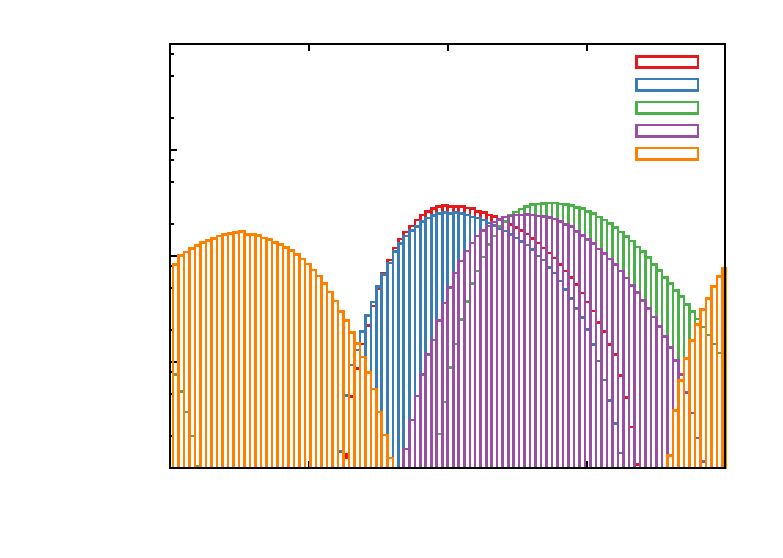
\includegraphics{images/unbound-mass-vs-phi}}%
    \gplfronttext
  \end{picture}%
\endgroup

	\caption[Angular distribution (in $\phi$) of the ejecta]{
		Angular distribution (in $\phi$) of the ejecta 5 ms after merger.  The ejecta spans approximately half of the zonal sky, with an angle of $\delta \phi \sim (0.99-1.13) \pi$, where M12-M7-S9-SFHo is the smallest and M12-M7-S9-FSU21 has the widest arc.
	}
	\label{fig:phihisto}
\end{figure}

\begin{figure}
	\centering
	% GNUPLOT: LaTeX picture with Postscript
\begingroup
  \makeatletter
  \providecommand\color[2][]{%
    \GenericError{(gnuplot) \space\space\space\@spaces}{%
      Package color not loaded in conjunction with
      terminal option `colourtext'%
    }{See the gnuplot documentation for explanation.%
    }{Either use 'blacktext' in gnuplot or load the package
      color.sty in LaTeX.}%
    \renewcommand\color[2][]{}%
  }%
  \providecommand\includegraphics[2][]{%
    \GenericError{(gnuplot) \space\space\space\@spaces}{%
      Package graphicx or graphics not loaded%
    }{See the gnuplot documentation for explanation.%
    }{The gnuplot epslatex terminal needs graphicx.sty or graphics.sty.}%
    \renewcommand\includegraphics[2][]{}%
  }%
  \providecommand\rotatebox[2]{#2}%
  \@ifundefined{ifGPcolor}{%
    \newif\ifGPcolor
    \GPcolortrue
  }{}%
  \@ifundefined{ifGPblacktext}{%
    \newif\ifGPblacktext
    \GPblacktexttrue
  }{}%
  % define a \g@addto@macro without @ in the name:
  \let\gplgaddtomacro\g@addto@macro
  % define empty templates for all commands taking text:
  \gdef\gplbacktext{}%
  \gdef\gplfronttext{}%
  \makeatother
  \ifGPblacktext
    % no textcolor at all
    \def\colorrgb#1{}%
    \def\colorgray#1{}%
  \else
    % gray or color?
    \ifGPcolor
      \def\colorrgb#1{\color[rgb]{#1}}%
      \def\colorgray#1{\color[gray]{#1}}%
      \expandafter\def\csname LTw\endcsname{\color{white}}%
      \expandafter\def\csname LTb\endcsname{\color{black}}%
      \expandafter\def\csname LTa\endcsname{\color{black}}%
      \expandafter\def\csname LT0\endcsname{\color[rgb]{1,0,0}}%
      \expandafter\def\csname LT1\endcsname{\color[rgb]{0,1,0}}%
      \expandafter\def\csname LT2\endcsname{\color[rgb]{0,0,1}}%
      \expandafter\def\csname LT3\endcsname{\color[rgb]{1,0,1}}%
      \expandafter\def\csname LT4\endcsname{\color[rgb]{0,1,1}}%
      \expandafter\def\csname LT5\endcsname{\color[rgb]{1,1,0}}%
      \expandafter\def\csname LT6\endcsname{\color[rgb]{0,0,0}}%
      \expandafter\def\csname LT7\endcsname{\color[rgb]{1,0.3,0}}%
      \expandafter\def\csname LT8\endcsname{\color[rgb]{0.5,0.5,0.5}}%
    \else
      % gray
      \def\colorrgb#1{\color{black}}%
      \def\colorgray#1{\color[gray]{#1}}%
      \expandafter\def\csname LTw\endcsname{\color{white}}%
      \expandafter\def\csname LTb\endcsname{\color{black}}%
      \expandafter\def\csname LTa\endcsname{\color{black}}%
      \expandafter\def\csname LT0\endcsname{\color{black}}%
      \expandafter\def\csname LT1\endcsname{\color{black}}%
      \expandafter\def\csname LT2\endcsname{\color{black}}%
      \expandafter\def\csname LT3\endcsname{\color{black}}%
      \expandafter\def\csname LT4\endcsname{\color{black}}%
      \expandafter\def\csname LT5\endcsname{\color{black}}%
      \expandafter\def\csname LT6\endcsname{\color{black}}%
      \expandafter\def\csname LT7\endcsname{\color{black}}%
      \expandafter\def\csname LT8\endcsname{\color{black}}%
    \fi
  \fi
  \setlength{\unitlength}{0.0500bp}%
  \begin{picture}(7200.00,5040.00)%
    \gplgaddtomacro\gplbacktext{%
      \csname LTb\endcsname%
      \put(1342,704){\makebox(0,0)[r]{\strut{} 1e-05}}%
      \put(1342,1722){\makebox(0,0)[r]{\strut{} 0.0001}}%
      \put(1342,2740){\makebox(0,0)[r]{\strut{} 0.001}}%
      \put(1342,3757){\makebox(0,0)[r]{\strut{} 0.01}}%
      \put(1342,4775){\makebox(0,0)[r]{\strut{} 0.1}}%
      \put(1474,484){\makebox(0,0){\strut{}-1}}%
      \put(2806,484){\makebox(0,0){\strut{}-0.5}}%
      \put(4139,484){\makebox(0,0){\strut{} 0}}%
      \put(5471,484){\makebox(0,0){\strut{} 0.5}}%
      \put(6803,484){\makebox(0,0){\strut{} 1}}%
      \put(176,2739){\rotatebox{-270}{\makebox(0,0){\strut{}$\log_{10}(M_{\rm ej})$ ($M_{\odot}$)}}}%
      \put(4138,154){\makebox(0,0){\strut{}$\cos(\theta)$}}%
    }%
    \gplgaddtomacro\gplfronttext{%
      \csname LTb\endcsname%
      \put(2461,4602){\makebox(0,0)[l]{\strut{}M12-M7-S9-DD2}}%
      \csname LTb\endcsname%
      \put(2461,4382){\makebox(0,0)[l]{\strut{}M14-M7-S9-DD2}}%
      \csname LTb\endcsname%
      \put(2461,4162){\makebox(0,0)[l]{\strut{}M12-M7-S9-FSU21}}%
      \csname LTb\endcsname%
      \put(2461,3942){\makebox(0,0)[l]{\strut{}M14-M7-S9-FSU21}}%
      \csname LTb\endcsname%
      \put(2461,3722){\makebox(0,0)[l]{\strut{}M12-M7-S9-SFHo}}%
    }%
    \gplbacktext
    \put(0,0){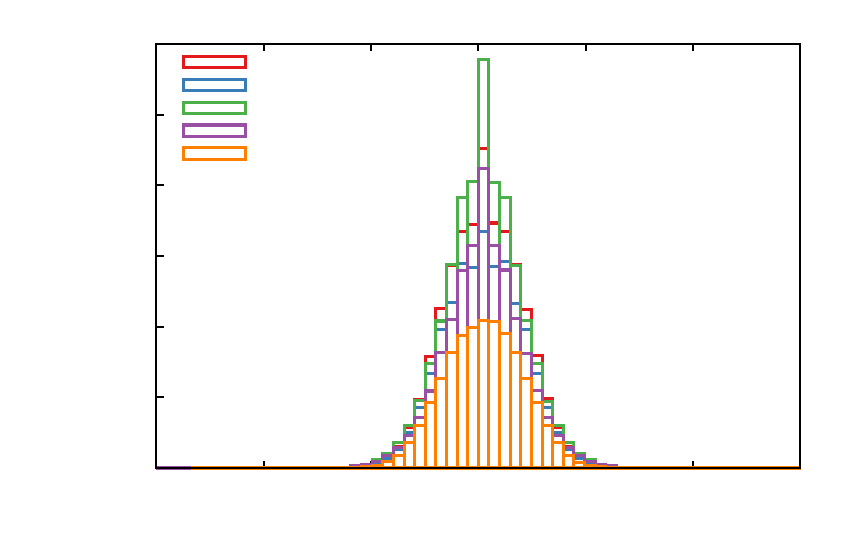
\includegraphics{images/unbound-mass-vs-costheta}}%
    \gplfronttext
  \end{picture}%
\endgroup

	\caption[Angular distribution (in $\theta$) of the ejecta]{
		Angular distribution (in $\theta$) of the ejecta 5 ms after merger.  
		Most of the ejecta matter is constrained around the equator, within $|\theta| \leq \pi/4$ and all of it is constrained with $|\theta| \leq \pi/2$.
	}
	\label{fig:costhetahisto}
\end{figure}


In addition, the ejecta geometry plays an integral role in the kilonova properties.  
In Figures \ref{fig:phihisto} and \ref{fig:costhetahisto}, we show the angular distribution of the ejecta in a spherical coordinate system in the inertial frame, where $\cos(\theta) = 0$ corresponds to the equator.  
Our results are consistent with previous black hole neutron star simulations, where the unbound material form a crescent with an opening zonal angle $\sym \pi$ and meridional angle $\sym \pi/4$.


\section{Post-merger remnant: formation of the protodisk and fallback}
\label{sec:disk-analysis}

Accretion of the fluid happens at a maximal rate during the merger. 
Around $ \sim 2.5$ ms after merger, this rapid accretion rate onto the black hole begins to slow and the average temperature of the fluid begins to reach a local minimum.
In our simulations, this window was the most difficult epoch of the merger, as the rate of expansion in the tail and then circularization are the horizon led to the creation of thousands of subdomains. 
\footnote{
We experienced an overwhelming number of memory issues here, and had to constantly but conservatively increase the number of computer processor cores used in each simulation.
That is, the number of fluid subdomains per processor quickly increased by a factor of (up to) six, requiring diligence in monitoring domain creation and increasing the requisite number of processors to improve the load balancing.
Performance suffers the worst during and shortly after merger, and makes gains as the resolution (i.e. subdomain size) was allowed to be lowered (increased) after maximal accretion and after circularization.  
For example, between the beginning of the plunge and the first derefinement, all simulations required $\sim 450000$ CPU hours to evolve 1 ms of merger (where timesteps shrink to nanoseconds), while the entire duration of the inspiral ($\sim 15 - 20$ ms) was performed with one 10th of this effort. 
}
Within the same timescale, the fluid eventually self-intersects when the higher density leading edge of the tail shocks against less dense fluid in the wider, bound portion of the tail.
This drives the fluid to slowly circularize into an early-evolution accretion disk, or protodisk.
On the timescale of $\sim 10-20$ ms post-merger, the protodisk continues to accrete, but also slowly cultivating fallback material from the bound portion of the tail.
The peak of the surface density of the disk begins to gradually advance outwards from the black hole horizon.
The disk secularizes from the tail over this $\sim 10$ ms period,
eventually forming an axisymmetric disk that could be evolved on much longer timescales if magnetic effects or an equivalent artificial viscosity scheme were added.

\begin{figure}
	\centering
	% GNUPLOT: LaTeX picture with Postscript
\begingroup
  \makeatletter
  \providecommand\color[2][]{%
    \GenericError{(gnuplot) \space\space\space\@spaces}{%
      Package color not loaded in conjunction with
      terminal option `colourtext'%
    }{See the gnuplot documentation for explanation.%
    }{Either use 'blacktext' in gnuplot or load the package
      color.sty in LaTeX.}%
    \renewcommand\color[2][]{}%
  }%
  \providecommand\includegraphics[2][]{%
    \GenericError{(gnuplot) \space\space\space\@spaces}{%
      Package graphicx or graphics not loaded%
    }{See the gnuplot documentation for explanation.%
    }{The gnuplot epslatex terminal needs graphicx.sty or graphics.sty.}%
    \renewcommand\includegraphics[2][]{}%
  }%
  \providecommand\rotatebox[2]{#2}%
  \@ifundefined{ifGPcolor}{%
    \newif\ifGPcolor
    \GPcolortrue
  }{}%
  \@ifundefined{ifGPblacktext}{%
    \newif\ifGPblacktext
    \GPblacktexttrue
  }{}%
  % define a \g@addto@macro without @ in the name:
  \let\gplgaddtomacro\g@addto@macro
  % define empty templates for all commands taking text:
  \gdef\gplbacktext{}%
  \gdef\gplfronttext{}%
  \makeatother
  \ifGPblacktext
    % no textcolor at all
    \def\colorrgb#1{}%
    \def\colorgray#1{}%
  \else
    % gray or color?
    \ifGPcolor
      \def\colorrgb#1{\color[rgb]{#1}}%
      \def\colorgray#1{\color[gray]{#1}}%
      \expandafter\def\csname LTw\endcsname{\color{white}}%
      \expandafter\def\csname LTb\endcsname{\color{black}}%
      \expandafter\def\csname LTa\endcsname{\color{black}}%
      \expandafter\def\csname LT0\endcsname{\color[rgb]{1,0,0}}%
      \expandafter\def\csname LT1\endcsname{\color[rgb]{0,1,0}}%
      \expandafter\def\csname LT2\endcsname{\color[rgb]{0,0,1}}%
      \expandafter\def\csname LT3\endcsname{\color[rgb]{1,0,1}}%
      \expandafter\def\csname LT4\endcsname{\color[rgb]{0,1,1}}%
      \expandafter\def\csname LT5\endcsname{\color[rgb]{1,1,0}}%
      \expandafter\def\csname LT6\endcsname{\color[rgb]{0,0,0}}%
      \expandafter\def\csname LT7\endcsname{\color[rgb]{1,0.3,0}}%
      \expandafter\def\csname LT8\endcsname{\color[rgb]{0.5,0.5,0.5}}%
    \else
      % gray
      \def\colorrgb#1{\color{black}}%
      \def\colorgray#1{\color[gray]{#1}}%
      \expandafter\def\csname LTw\endcsname{\color{white}}%
      \expandafter\def\csname LTb\endcsname{\color{black}}%
      \expandafter\def\csname LTa\endcsname{\color{black}}%
      \expandafter\def\csname LT0\endcsname{\color{black}}%
      \expandafter\def\csname LT1\endcsname{\color{black}}%
      \expandafter\def\csname LT2\endcsname{\color{black}}%
      \expandafter\def\csname LT3\endcsname{\color{black}}%
      \expandafter\def\csname LT4\endcsname{\color{black}}%
      \expandafter\def\csname LT5\endcsname{\color{black}}%
      \expandafter\def\csname LT6\endcsname{\color{black}}%
      \expandafter\def\csname LT7\endcsname{\color{black}}%
      \expandafter\def\csname LT8\endcsname{\color{black}}%
    \fi
  \fi
  \setlength{\unitlength}{0.0500bp}%
  \begin{picture}(7920.00,5040.00)%
    \gplgaddtomacro\gplbacktext{%
      \csname LTb\endcsname%
      \put(1210,1130){\makebox(0,0)[r]{\strut{} 1e+11}}%
      \put(1210,3166){\makebox(0,0)[r]{\strut{} 1e+12}}%
      \put(1342,484){\makebox(0,0){\strut{} 20}}%
      \put(2029,484){\makebox(0,0){\strut{} 30}}%
      \put(2716,484){\makebox(0,0){\strut{} 40}}%
      \put(3402,484){\makebox(0,0){\strut{} 50}}%
      \put(4089,484){\makebox(0,0){\strut{} 60}}%
      \put(4776,484){\makebox(0,0){\strut{} 70}}%
      \put(5463,484){\makebox(0,0){\strut{} 80}}%
      \put(6149,484){\makebox(0,0){\strut{} 90}}%
      \put(6836,484){\makebox(0,0){\strut{} 100}}%
      \put(7523,484){\makebox(0,0){\strut{} 110}}%
      \put(176,2739){\rotatebox{-270}{\makebox(0,0){\strut{}$\log_{10}(\rho_0) {\rm (cgs)}$}}}%
      \put(4432,154){\makebox(0,0){\strut{}$ R ({\rm km}) $}}%
    }%
    \gplgaddtomacro\gplfronttext{%
      \csname LTb\endcsname%
      \put(6536,4602){\makebox(0,0)[r]{\strut{}M12-M7-S9-DD2}}%
      \csname LTb\endcsname%
      \put(6536,4382){\makebox(0,0)[r]{\strut{}M14-M7-S9-DD2}}%
      \csname LTb\endcsname%
      \put(6536,4162){\makebox(0,0)[r]{\strut{}M12-M7-S9-FSU21}}%
      \csname LTb\endcsname%
      \put(6536,3942){\makebox(0,0)[r]{\strut{}M14-M7-S9-FSU21}}%
      \csname LTb\endcsname%
      \put(6536,3722){\makebox(0,0)[r]{\strut{}M12-M7-S9-SFHo}}%
    }%
    \gplbacktext
    \put(0,0){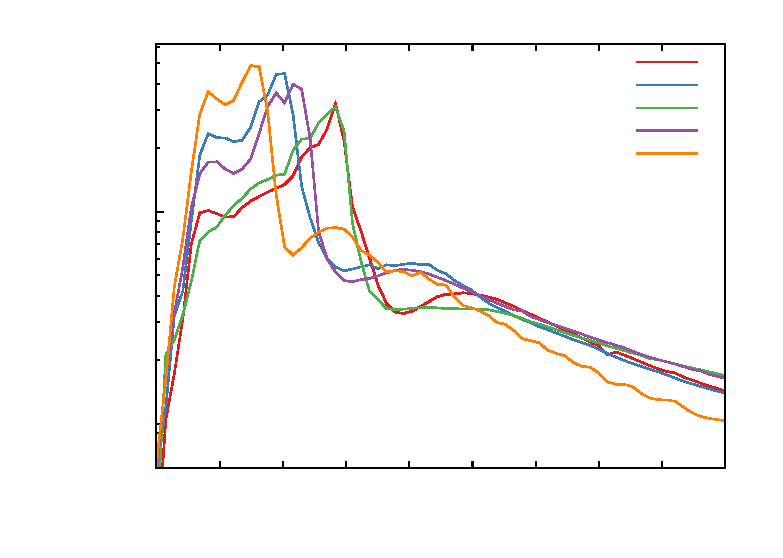
\includegraphics{images/density-of-disk}}%
    \gplfronttext
  \end{picture}%
\endgroup

	\caption[Density profiles of the protodisks 5 ms after merger]{
		Averaged density profiles of the protodisks 5 ms after merger.  The densest zone in the disks ranges $R \sim 30 - 50 {\rm km}$ from the center of the black hole (with a predicted final ISCO radius of $\sym 24 {\rm km}$).  
	}
	\label{fig:diskdensities}
\end{figure}

Because most of our simulations have yet to reach this approximate time of axisymmetrization ($\sim 10$ ms post-merger) where one normally measures the properties of the disk, we will at least analyze the protodisk and fallback properties at 5 ms past merger.
One argument we can \textit{a priori} make for this is demonstrated in [cite:foucart2014], where simulations with more massive post-
merger remnants rapidly form massive, hot inner disks and have less variability during the first $5-10$ ms, as with ours and in comparison to those with less massive disks yields.
The disk mass predictions of Equation \ref{e:mass_disk} are for the total bound baryonic mass remaining in the system, which include both the protodisk and fallback matter.
Roughly speaking, we define the disk as the bound matter having a minimum threshold of rotational velocity (i.e., $-1 < v_r/v_\phi < 0$) and a minimum temperature ($T>0.1$) in order to ditinguish the disk from the fallback,
while the fallback material is the remaining bound matter in the tidal tail.
At 5 ms past merger, our simulations yield a wide range of fallback material, in the range of $(32 - 71)\%$ fallback.  
The lowest fallback yield is that of the M12-M7-S9-SFHo model, while both $1.4 M_\odot$ models have the most amount of infalling matter at this time.
This is because more compact stars disrupt closer to the ISCO.

\begin{figure}
	\centering
	% GNUPLOT: LaTeX picture with Postscript
\begingroup
  \makeatletter
  \providecommand\color[2][]{%
    \GenericError{(gnuplot) \space\space\space\@spaces}{%
      Package color not loaded in conjunction with
      terminal option `colourtext'%
    }{See the gnuplot documentation for explanation.%
    }{Either use 'blacktext' in gnuplot or load the package
      color.sty in LaTeX.}%
    \renewcommand\color[2][]{}%
  }%
  \providecommand\includegraphics[2][]{%
    \GenericError{(gnuplot) \space\space\space\@spaces}{%
      Package graphicx or graphics not loaded%
    }{See the gnuplot documentation for explanation.%
    }{The gnuplot epslatex terminal needs graphicx.sty or graphics.sty.}%
    \renewcommand\includegraphics[2][]{}%
  }%
  \providecommand\rotatebox[2]{#2}%
  \@ifundefined{ifGPcolor}{%
    \newif\ifGPcolor
    \GPcolortrue
  }{}%
  \@ifundefined{ifGPblacktext}{%
    \newif\ifGPblacktext
    \GPblacktexttrue
  }{}%
  % define a \g@addto@macro without @ in the name:
  \let\gplgaddtomacro\g@addto@macro
  % define empty templates for all commands taking text:
  \gdef\gplbacktext{}%
  \gdef\gplfronttext{}%
  \makeatother
  \ifGPblacktext
    % no textcolor at all
    \def\colorrgb#1{}%
    \def\colorgray#1{}%
  \else
    % gray or color?
    \ifGPcolor
      \def\colorrgb#1{\color[rgb]{#1}}%
      \def\colorgray#1{\color[gray]{#1}}%
      \expandafter\def\csname LTw\endcsname{\color{white}}%
      \expandafter\def\csname LTb\endcsname{\color{black}}%
      \expandafter\def\csname LTa\endcsname{\color{black}}%
      \expandafter\def\csname LT0\endcsname{\color[rgb]{1,0,0}}%
      \expandafter\def\csname LT1\endcsname{\color[rgb]{0,1,0}}%
      \expandafter\def\csname LT2\endcsname{\color[rgb]{0,0,1}}%
      \expandafter\def\csname LT3\endcsname{\color[rgb]{1,0,1}}%
      \expandafter\def\csname LT4\endcsname{\color[rgb]{0,1,1}}%
      \expandafter\def\csname LT5\endcsname{\color[rgb]{1,1,0}}%
      \expandafter\def\csname LT6\endcsname{\color[rgb]{0,0,0}}%
      \expandafter\def\csname LT7\endcsname{\color[rgb]{1,0.3,0}}%
      \expandafter\def\csname LT8\endcsname{\color[rgb]{0.5,0.5,0.5}}%
    \else
      % gray
      \def\colorrgb#1{\color{black}}%
      \def\colorgray#1{\color[gray]{#1}}%
      \expandafter\def\csname LTw\endcsname{\color{white}}%
      \expandafter\def\csname LTb\endcsname{\color{black}}%
      \expandafter\def\csname LTa\endcsname{\color{black}}%
      \expandafter\def\csname LT0\endcsname{\color{black}}%
      \expandafter\def\csname LT1\endcsname{\color{black}}%
      \expandafter\def\csname LT2\endcsname{\color{black}}%
      \expandafter\def\csname LT3\endcsname{\color{black}}%
      \expandafter\def\csname LT4\endcsname{\color{black}}%
      \expandafter\def\csname LT5\endcsname{\color{black}}%
      \expandafter\def\csname LT6\endcsname{\color{black}}%
      \expandafter\def\csname LT7\endcsname{\color{black}}%
      \expandafter\def\csname LT8\endcsname{\color{black}}%
    \fi
  \fi
  \setlength{\unitlength}{0.0500bp}%
  \begin{picture}(7920.00,5040.00)%
    \gplgaddtomacro\gplbacktext{%
      \csname LTb\endcsname%
      \put(814,704){\makebox(0,0)[r]{\strut{} 0}}%
      \put(814,1286){\makebox(0,0)[r]{\strut{} 2}}%
      \put(814,1867){\makebox(0,0)[r]{\strut{} 4}}%
      \put(814,2449){\makebox(0,0)[r]{\strut{} 6}}%
      \put(814,3030){\makebox(0,0)[r]{\strut{} 8}}%
      \put(814,3612){\makebox(0,0)[r]{\strut{} 10}}%
      \put(814,4193){\makebox(0,0)[r]{\strut{} 12}}%
      \put(814,4775){\makebox(0,0)[r]{\strut{} 14}}%
      \put(946,484){\makebox(0,0){\strut{} 20}}%
      \put(1677,484){\makebox(0,0){\strut{} 30}}%
      \put(2408,484){\makebox(0,0){\strut{} 40}}%
      \put(3138,484){\makebox(0,0){\strut{} 50}}%
      \put(3869,484){\makebox(0,0){\strut{} 60}}%
      \put(4600,484){\makebox(0,0){\strut{} 70}}%
      \put(5331,484){\makebox(0,0){\strut{} 80}}%
      \put(6061,484){\makebox(0,0){\strut{} 90}}%
      \put(6792,484){\makebox(0,0){\strut{} 100}}%
      \put(7523,484){\makebox(0,0){\strut{} 110}}%
      \put(176,2739){\rotatebox{-270}{\makebox(0,0){\strut{}$ T ({\rm MeV}) $}}}%
      \put(4234,154){\makebox(0,0){\strut{}$ R ({\rm km}) $}}%
    }%
    \gplgaddtomacro\gplfronttext{%
      \csname LTb\endcsname%
      \put(6536,4602){\makebox(0,0)[r]{\strut{}M12-M7-S9-DD2}}%
      \csname LTb\endcsname%
      \put(6536,4382){\makebox(0,0)[r]{\strut{}M14-M7-S9-DD2}}%
      \csname LTb\endcsname%
      \put(6536,4162){\makebox(0,0)[r]{\strut{}M12-M7-S9-FSU21}}%
      \csname LTb\endcsname%
      \put(6536,3942){\makebox(0,0)[r]{\strut{}M14-M7-S9-FSU21}}%
      \csname LTb\endcsname%
      \put(6536,3722){\makebox(0,0)[r]{\strut{}M12-M7-S9-SFHo}}%
    }%
    \gplbacktext
    \put(0,0){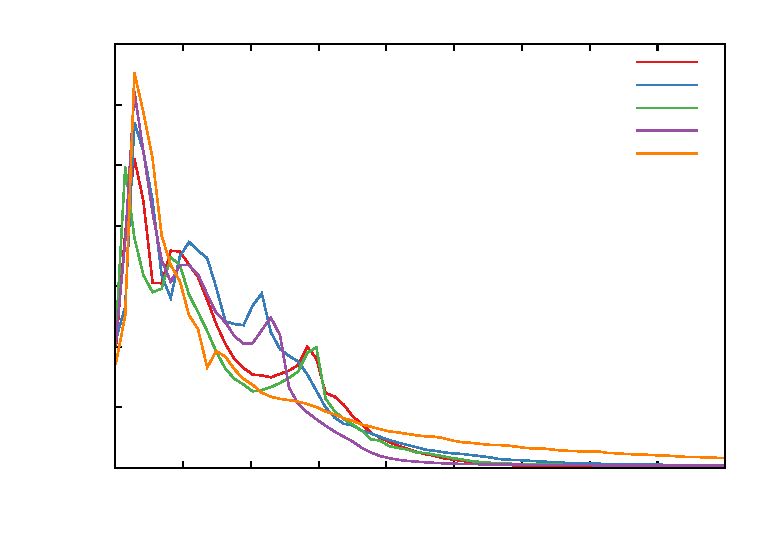
\includegraphics{images/temperature-of-disk}}%
    \gplfronttext
  \end{picture}%
\endgroup

	\caption[Temperature profiles of the protodisks 5 ms after merger]{
		Averaged temperature profiles of the protodisks 5 ms after merger.  The temperature near the peaks of the density profiles is $T \sim (4-7) {\rm MeV}$, and becomes quite cool in the low density region ($r>75 {\rm km}$) outside the disk.  
	}
	\label{fig:disktemps}
\end{figure}

We see that in Figure \ref{fig:diskdensities}, most of the material is within 
$25 {\rm km} < r < 75{\rm km}$ for all models and drops off exponentially after that upper-bound, while the peak of the matter distribution is $r _{\rm disk} \sim (30 - 50) {\rm km}$.  
The composition is roughly constant outside the ISCO, $Y_e \sim 0.05 - 0.08$.  The temperature at the peak of the matter distribution varies as $T \sim (4-7) {\rm MeV}$ between runs, with M12-M7-S9-SFHo having the hottest protodisk and being only slightly more protonized. 
The neutrino luminosities at this time are high, $L_\nu \sim (1.5 - 5.5) \times 10^{53} {\rm egs/s}$, 



\begin{figure}
	\centering
	% GNUPLOT: LaTeX picture with Postscript
\begingroup
  \makeatletter
  \providecommand\color[2][]{%
    \GenericError{(gnuplot) \space\space\space\@spaces}{%
      Package color not loaded in conjunction with
      terminal option `colourtext'%
    }{See the gnuplot documentation for explanation.%
    }{Either use 'blacktext' in gnuplot or load the package
      color.sty in LaTeX.}%
    \renewcommand\color[2][]{}%
  }%
  \providecommand\includegraphics[2][]{%
    \GenericError{(gnuplot) \space\space\space\@spaces}{%
      Package graphicx or graphics not loaded%
    }{See the gnuplot documentation for explanation.%
    }{The gnuplot epslatex terminal needs graphicx.sty or graphics.sty.}%
    \renewcommand\includegraphics[2][]{}%
  }%
  \providecommand\rotatebox[2]{#2}%
  \@ifundefined{ifGPcolor}{%
    \newif\ifGPcolor
    \GPcolortrue
  }{}%
  \@ifundefined{ifGPblacktext}{%
    \newif\ifGPblacktext
    \GPblacktexttrue
  }{}%
  % define a \g@addto@macro without @ in the name:
  \let\gplgaddtomacro\g@addto@macro
  % define empty templates for all commands taking text:
  \gdef\gplbacktext{}%
  \gdef\gplfronttext{}%
  \makeatother
  \ifGPblacktext
    % no textcolor at all
    \def\colorrgb#1{}%
    \def\colorgray#1{}%
  \else
    % gray or color?
    \ifGPcolor
      \def\colorrgb#1{\color[rgb]{#1}}%
      \def\colorgray#1{\color[gray]{#1}}%
      \expandafter\def\csname LTw\endcsname{\color{white}}%
      \expandafter\def\csname LTb\endcsname{\color{black}}%
      \expandafter\def\csname LTa\endcsname{\color{black}}%
      \expandafter\def\csname LT0\endcsname{\color[rgb]{1,0,0}}%
      \expandafter\def\csname LT1\endcsname{\color[rgb]{0,1,0}}%
      \expandafter\def\csname LT2\endcsname{\color[rgb]{0,0,1}}%
      \expandafter\def\csname LT3\endcsname{\color[rgb]{1,0,1}}%
      \expandafter\def\csname LT4\endcsname{\color[rgb]{0,1,1}}%
      \expandafter\def\csname LT5\endcsname{\color[rgb]{1,1,0}}%
      \expandafter\def\csname LT6\endcsname{\color[rgb]{0,0,0}}%
      \expandafter\def\csname LT7\endcsname{\color[rgb]{1,0.3,0}}%
      \expandafter\def\csname LT8\endcsname{\color[rgb]{0.5,0.5,0.5}}%
    \else
      % gray
      \def\colorrgb#1{\color{black}}%
      \def\colorgray#1{\color[gray]{#1}}%
      \expandafter\def\csname LTw\endcsname{\color{white}}%
      \expandafter\def\csname LTb\endcsname{\color{black}}%
      \expandafter\def\csname LTa\endcsname{\color{black}}%
      \expandafter\def\csname LT0\endcsname{\color{black}}%
      \expandafter\def\csname LT1\endcsname{\color{black}}%
      \expandafter\def\csname LT2\endcsname{\color{black}}%
      \expandafter\def\csname LT3\endcsname{\color{black}}%
      \expandafter\def\csname LT4\endcsname{\color{black}}%
      \expandafter\def\csname LT5\endcsname{\color{black}}%
      \expandafter\def\csname LT6\endcsname{\color{black}}%
      \expandafter\def\csname LT7\endcsname{\color{black}}%
      \expandafter\def\csname LT8\endcsname{\color{black}}%
    \fi
  \fi
  \setlength{\unitlength}{0.0500bp}%
  \begin{picture}(7920.00,5040.00)%
    \gplgaddtomacro\gplbacktext{%
      \csname LTb\endcsname%
      \put(1078,704){\makebox(0,0)[r]{\strut{} 0}}%
      \put(1078,1213){\makebox(0,0)[r]{\strut{} 0.05}}%
      \put(1078,1722){\makebox(0,0)[r]{\strut{} 0.1}}%
      \put(1078,2231){\makebox(0,0)[r]{\strut{} 0.15}}%
      \put(1078,2740){\makebox(0,0)[r]{\strut{} 0.2}}%
      \put(1078,3248){\makebox(0,0)[r]{\strut{} 0.25}}%
      \put(1078,3757){\makebox(0,0)[r]{\strut{} 0.3}}%
      \put(1078,4266){\makebox(0,0)[r]{\strut{} 0.35}}%
      \put(1078,4775){\makebox(0,0)[r]{\strut{} 0.4}}%
      \put(1210,484){\makebox(0,0){\strut{} 20}}%
      \put(1911,484){\makebox(0,0){\strut{} 30}}%
      \put(2613,484){\makebox(0,0){\strut{} 40}}%
      \put(3314,484){\makebox(0,0){\strut{} 50}}%
      \put(4016,484){\makebox(0,0){\strut{} 60}}%
      \put(4717,484){\makebox(0,0){\strut{} 70}}%
      \put(5419,484){\makebox(0,0){\strut{} 80}}%
      \put(6120,484){\makebox(0,0){\strut{} 90}}%
      \put(6822,484){\makebox(0,0){\strut{} 100}}%
      \put(7523,484){\makebox(0,0){\strut{} 110}}%
      \put(176,2739){\rotatebox{-270}{\makebox(0,0){\strut{}$ Y_e $}}}%
      \put(4366,154){\makebox(0,0){\strut{}$ R ({\rm km}) $}}%
    }%
    \gplgaddtomacro\gplfronttext{%
      \csname LTb\endcsname%
      \put(6536,4602){\makebox(0,0)[r]{\strut{}M12-M7-S9-DD2}}%
      \csname LTb\endcsname%
      \put(6536,4382){\makebox(0,0)[r]{\strut{}M14-M7-S9-DD2}}%
      \csname LTb\endcsname%
      \put(6536,4162){\makebox(0,0)[r]{\strut{}M12-M7-S9-FSU21}}%
      \csname LTb\endcsname%
      \put(6536,3942){\makebox(0,0)[r]{\strut{}M14-M7-S9-FSU21}}%
      \csname LTb\endcsname%
      \put(6536,3722){\makebox(0,0)[r]{\strut{}M12-M7-S9-SFHo}}%
    }%
    \gplbacktext
    \put(0,0){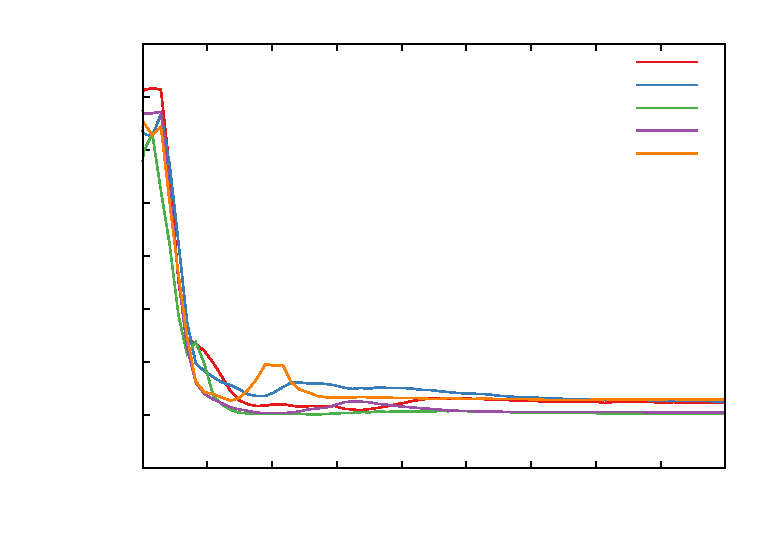
\includegraphics{images/composition-of-disk}}%
    \gplfronttext
  \end{picture}%
\endgroup

	\caption[Radial compositions of the protodisks 5 ms after merger]{
	Averaged radial compositions of the protodisks 5 ms after merger.  
	The fluid is highly protonized ($Ye > 0.25$) near the black hole horizon, while nearly constant in the circularizing portion of the disk ($Y_e \sim 0.05 - 0.08$).
	}
	\label{fig:diskYes}
\end{figure}

\begin{figure}
	\centering
	% GNUPLOT: LaTeX picture with Postscript
\begingroup
  \makeatletter
  \providecommand\color[2][]{%
    \GenericError{(gnuplot) \space\space\space\@spaces}{%
      Package color not loaded in conjunction with
      terminal option `colourtext'%
    }{See the gnuplot documentation for explanation.%
    }{Either use 'blacktext' in gnuplot or load the package
      color.sty in LaTeX.}%
    \renewcommand\color[2][]{}%
  }%
  \providecommand\includegraphics[2][]{%
    \GenericError{(gnuplot) \space\space\space\@spaces}{%
      Package graphicx or graphics not loaded%
    }{See the gnuplot documentation for explanation.%
    }{The gnuplot epslatex terminal needs graphicx.sty or graphics.sty.}%
    \renewcommand\includegraphics[2][]{}%
  }%
  \providecommand\rotatebox[2]{#2}%
  \@ifundefined{ifGPcolor}{%
    \newif\ifGPcolor
    \GPcolortrue
  }{}%
  \@ifundefined{ifGPblacktext}{%
    \newif\ifGPblacktext
    \GPblacktexttrue
  }{}%
  % define a \g@addto@macro without @ in the name:
  \let\gplgaddtomacro\g@addto@macro
  % define empty templates for all commands taking text:
  \gdef\gplbacktext{}%
  \gdef\gplfronttext{}%
  \makeatother
  \ifGPblacktext
    % no textcolor at all
    \def\colorrgb#1{}%
    \def\colorgray#1{}%
  \else
    % gray or color?
    \ifGPcolor
      \def\colorrgb#1{\color[rgb]{#1}}%
      \def\colorgray#1{\color[gray]{#1}}%
      \expandafter\def\csname LTw\endcsname{\color{white}}%
      \expandafter\def\csname LTb\endcsname{\color{black}}%
      \expandafter\def\csname LTa\endcsname{\color{black}}%
      \expandafter\def\csname LT0\endcsname{\color[rgb]{1,0,0}}%
      \expandafter\def\csname LT1\endcsname{\color[rgb]{0,1,0}}%
      \expandafter\def\csname LT2\endcsname{\color[rgb]{0,0,1}}%
      \expandafter\def\csname LT3\endcsname{\color[rgb]{1,0,1}}%
      \expandafter\def\csname LT4\endcsname{\color[rgb]{0,1,1}}%
      \expandafter\def\csname LT5\endcsname{\color[rgb]{1,1,0}}%
      \expandafter\def\csname LT6\endcsname{\color[rgb]{0,0,0}}%
      \expandafter\def\csname LT7\endcsname{\color[rgb]{1,0.3,0}}%
      \expandafter\def\csname LT8\endcsname{\color[rgb]{0.5,0.5,0.5}}%
    \else
      % gray
      \def\colorrgb#1{\color{black}}%
      \def\colorgray#1{\color[gray]{#1}}%
      \expandafter\def\csname LTw\endcsname{\color{white}}%
      \expandafter\def\csname LTb\endcsname{\color{black}}%
      \expandafter\def\csname LTa\endcsname{\color{black}}%
      \expandafter\def\csname LT0\endcsname{\color{black}}%
      \expandafter\def\csname LT1\endcsname{\color{black}}%
      \expandafter\def\csname LT2\endcsname{\color{black}}%
      \expandafter\def\csname LT3\endcsname{\color{black}}%
      \expandafter\def\csname LT4\endcsname{\color{black}}%
      \expandafter\def\csname LT5\endcsname{\color{black}}%
      \expandafter\def\csname LT6\endcsname{\color{black}}%
      \expandafter\def\csname LT7\endcsname{\color{black}}%
      \expandafter\def\csname LT8\endcsname{\color{black}}%
    \fi
  \fi
  \setlength{\unitlength}{0.0500bp}%
  \begin{picture}(7920.00,5040.00)%
    \gplgaddtomacro\gplbacktext{%
      \csname LTb\endcsname%
      \put(1210,704){\makebox(0,0)[r]{\strut{} 0}}%
      \put(1210,1156){\makebox(0,0)[r]{\strut{} 0.002}}%
      \put(1210,1609){\makebox(0,0)[r]{\strut{} 0.004}}%
      \put(1210,2061){\makebox(0,0)[r]{\strut{} 0.006}}%
      \put(1210,2513){\makebox(0,0)[r]{\strut{} 0.008}}%
      \put(1210,2966){\makebox(0,0)[r]{\strut{} 0.01}}%
      \put(1210,3418){\makebox(0,0)[r]{\strut{} 0.012}}%
      \put(1210,3870){\makebox(0,0)[r]{\strut{} 0.014}}%
      \put(1210,4323){\makebox(0,0)[r]{\strut{} 0.016}}%
      \put(1210,4775){\makebox(0,0)[r]{\strut{} 0.018}}%
      \put(1342,484){\makebox(0,0){\strut{} 20}}%
      \put(2029,484){\makebox(0,0){\strut{} 30}}%
      \put(2716,484){\makebox(0,0){\strut{} 40}}%
      \put(3402,484){\makebox(0,0){\strut{} 50}}%
      \put(4089,484){\makebox(0,0){\strut{} 60}}%
      \put(4776,484){\makebox(0,0){\strut{} 70}}%
      \put(5463,484){\makebox(0,0){\strut{} 80}}%
      \put(6149,484){\makebox(0,0){\strut{} 90}}%
      \put(6836,484){\makebox(0,0){\strut{} 100}}%
      \put(7523,484){\makebox(0,0){\strut{} 110}}%
      \put(176,2739){\rotatebox{-270}{\makebox(0,0){\strut{}$ S (k_{\rm B}) $}}}%
      \put(4432,154){\makebox(0,0){\strut{}$ R ({\rm km}) $}}%
    }%
    \gplgaddtomacro\gplfronttext{%
      \csname LTb\endcsname%
      \put(6536,4602){\makebox(0,0)[r]{\strut{}M12-M7-S9-DD2}}%
      \csname LTb\endcsname%
      \put(6536,4382){\makebox(0,0)[r]{\strut{}M14-M7-S9-DD2}}%
      \csname LTb\endcsname%
      \put(6536,4162){\makebox(0,0)[r]{\strut{}M12-M7-S9-FSU21}}%
      \csname LTb\endcsname%
      \put(6536,3942){\makebox(0,0)[r]{\strut{}M14-M7-S9-FSU21}}%
      \csname LTb\endcsname%
      \put(6536,3722){\makebox(0,0)[r]{\strut{}M12-M7-S9-SFHo}}%
    }%
    \gplbacktext
    \put(0,0){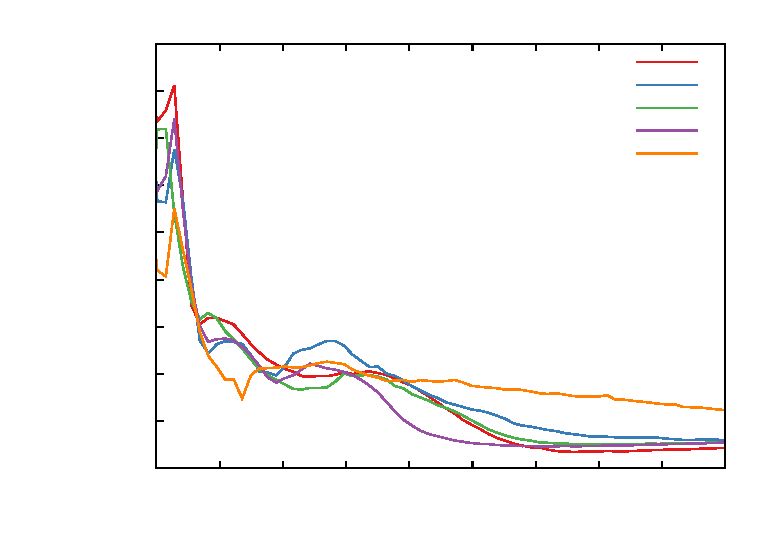
\includegraphics{images/entropy-of-disk}}%
    \gplfronttext
  \end{picture}%
\endgroup

	\caption[Average entropy of the protodisks 5 ms after merger]{
		Average entropy of the protodisks 5 ms after merger. \textbf{TODO}
	}
	\label{fig:diskentropies}
\end{figure}


\section{Discussion}
\label{sec:discussion}

The first simulations of neutron stars with multiple hot, temperature- and composition-dependent nuclear theory-based equations of state in black hole-neutron star mergers using a general relativistic fluid code were performed in this study.  
The mergers presented here all consider the same black hole parameters, with an orbitally aligned, relatively high black hole spin $\chi_{\rm BH} = 0.9$ and  mass $M_{\rm BH} = 7 M_\odot$, within the range of the most likely black hole masses.  
The neutron stars considered in this paper were evolved with the SFHo, DD2 and FSU2.1 equations of state with relatively low masses $M_{\rm NS} = (1.2,1.4) M_\odot$ over a wide range of compactnesess.  
These equations of state satisfy a number of observational, experimental and causal constraints.  
The ejecta of the five models that evolved far enough passed merger (for the fluid to circularize near the horizon) is very neutron-rich $Y_e = 0.05$, allowing for the robust production of heavy elements on the 2nd and 3rd peak of r-process nucleosynthesis.

We note that while we have implemented our improved algorithm to selectively evolve only non-vacuum subdomains, three of our models (M14-M17-S9-SFHo, M12-M17-S9-SFHx, and M14-M17-S9-SFHx) still had significant numerical error during merger. 
This is because our hot, compositio- dependent, tidally-disrupting material forms a much narrower tidal tail than other piecewise polytrope models.
An improvement to our algorithm would be to allow true adaptive mesh refinement, so that evolution subdomains could themselves shrink and expand given the average density gradient of the material inside.

\paragraph{Future work} 

The calculation of the gravitational waveform is in progress.  One simplification to the post-merger system is to  we are going to do is to turn off the fluid evolution and evolve only the metric quantities until the the waves propogate out to infinity.  For the neutrino emission, we did not include the effects of radiation transport in our simulations, which cannot be determnined by the relatively simple neutrino leakage scheme used in this work.  In order to capture an estimate of the production of electron-positron pairs in neutrino-driven winds near the spin axes of the black hole, evolving the fluid with a neutrino radiation code would improve the accuracy of the post-merger remnant evolution.  Furthermore, the effects of magnetic fields contribute heating through MRI turbulence.  Simulations of the post-merger remnant would be greatly enhanced with the inclusion of magnetohydrodynamics of an equivalent artificial viscosity scheme. 




\newpage

% Bibliography
\bibliography{references/References.bib}

\end{document}
